% !TEX TS-program = pdflatex
% !TEX encoding = UTF-8 Unicode

% This is a simple template for a LaTeX document using the "article" class.
% See "book", "report", "letter" for other types of document.

\documentclass[11pt]{article} % use larger type; default would be 10pt

\usepackage[utf8]{inputenc} % set input encoding (not needed with XeLaTeX)
\usepackage[english]{babel}
\usepackage{hyperref}
%\usepackage[cp1250]{inputenc}
%\usepackage[utf8]{inputenc}
\usepackage{latexsym}
\usepackage{amsfonts}
\usepackage{times}
\usepackage{xcolor}
\usepackage{graphicx}
\usepackage{crayola}
%\usepackage{datum}
\usepackage{xspace}
\usepackage{algorithmicx}
\usepackage{natbib}
\usepackage{authblk}
\usepackage{longtable}
\usepackage{rotating}
\usepackage{pdflscape}


\renewcommand{\textfraction}{.05}
\renewcommand{\topfraction}{.95}

\oddsidemargin 5pt \evensidemargin 5pt \marginparwidth 20pt
\marginparsep 10pt \topmargin -12 true mm \headheight 12pt \headsep 25pt
\textheight 23 true cm \textwidth 16 true cm
\columnsep 10pt \columnseprule 0pt

% title page --------------------------------------------------------------

\newcommand*{\affaddr}[1]{#1} % No op here. Customize it for different styles.
\newcommand*{\affmark}[1][*]{\textsuperscript{#1}}
\newcommand*{\email}[1]{\texttt{#1}}

\title{\LARGE\textbf{Social Network Analysis}\protect\\ The evolution of the field}
%\thanks{\textcolor{BrickRed}{\textbf{Applied Statistics}}, Ribno, 23-26. September 2018}

\author{%
Darja Maltseva\affmark[1], Vladimir Batagelj\affmark[1,2,3]\\
\affaddr{\affmark[1]NRU HSE Moscow}\\
\affaddr{\affmark[2]IMFM Ljubljana}\\
\affaddr{\affmark[3]IAM UP Koper}\\ \email{d.maltseva@gmail.com}\\
\email{vladimir.batagelj@fmf.uni-lj.si} %\\
%\affaddr{\LaTeX\ University}%
}
% \author{Darja Maljceva, Vladimir Batagelj  IMFM Ljubljana, IAM UP Koper, NRU HSE Moscow}


% user's macros ----------------------------------------------------------
\newcommand{\Pajek}{\texttt{\textbf{Pajek}}\xspace}
\newcommand{\WoSPajek}{\texttt{\textbf{WoS2Pajek}}\xspace}
%\newcommand{\Pajek}{Pajek}
\newcommand{\keyw}[1]{\textcolor{red}{\emph{#1}}}

\newcommand{\WA}{\mathbf{W\!\!A}}
\newcommand{\AW}{\mathbf{A\!\!W}}
\newcommand{\WK}{\mathbf{W\!K}}
\newcommand{\KW}{\mathbf{K\!W}}
\newcommand{\WC}{\mathbf{W\!C}}
\newcommand{\WJ}{\mathbf{W\!J}}
\newcommand{\Ci}{\mathbf{Cite}}
\newcommand{\Co}{\mathbf{Co}}
\newcommand{\Cn}{\mathbf{Cn}}
\newcommand{\Ct}{\mathbf{Ct}}
\newcommand{\N}{\mathbf{N}}
\newcommand{\NP}{N\!P}
%\newcommand{\diag}{\operatorname{diag}}
\newcommand{\sgn}{\operatorname{sgn}}
% \newcommand{\WA}{\mathbf{W\!A}}

\newcommand{\important}[1]{\textcolor{NavyBlue}{#1}}
\newcommand{\RR}{\Bbb{R}}
\newcommand{\NN}{\Bbb{N}}
\newcommand{\ZZ}{\Bbb{Z}}
\newcommand{\QQ}{\Bbb{Q}}
\newcommand{\network}[1]{\mathcal{#1}}
\newcommand{\vertices}[1]{\mathcal{#1}}
\newcommand{\edges}[1]{\mathcal{#1}}
\newcommand{\arcs}[1]{\mathcal{#1}}
\newcommand{\Net}{\network{N}}
\newcommand{\argmin}{\mathop{\mbox{argmin}}\nolimits}
\newcommand{\relation}[1]{\textbf{\emph{$\_\!\_$~#1~$\_\!\_$\,}}}
\newcommand{\functions}[1]{\mathcal{#1}}
\newcommand{\define}[1]{\emph{\textcolor{red}{#1}}}
\newcommand{\card}[1]{\mbox{card}(#1)}
\newcommand{\URL}[1]{{\footnotesize\texttt{#1}}}
\newcommand{\tita}[1]{\textit{#1}}      % italic
\newcommand{\cling}{\mathbf{C}}
\newcommand{\unitX}{\mbox{X}}
\newcommand{\unitY}{\mbox{Y}}
\newcommand{\unitZ}{\mbox{Z}}
\newcommand{\outdeg}{\mbox{outdeg}}
\newcommand{\indeg}{\mbox{indeg}}
\newcommand{\ato}{\mathrel{:=}}
\newcommand{\unit}{\mbox{X}}
\newcommand{\Units}{\vertices{U}}
\def\Min{\mathop{\mbox{Min}}\nolimits}
\def\Max{\mathop{\mbox{Max}}\nolimits}
\newcommand{\graph}[1]{\mathcal{#1}}
\newcommand{\function}[3]{#1\,{:}\ #2\to#3}
\newcommand{\Gph}{\network{G}}
\newcommand{\GphH}{\network{H}}
\newcommand{\Graph}{\mathbf{G}}
\newcommand{\tit}[1]{\textit{#1}}      % italic
\newcommand{\diag}{\mbox{diag}}
\newcommand{\func}[1]{\textit{#1}}
\newcommand{\Relation}[1]{\mathbf{#1}}
\newcommand{\Time}{\mathcal{T}}
%\newcommand{\cmdkey}{\raisebox{-.035em}{\includegraphics[height=.75em]{command.pdf}}}
\newcommand{\cmdkey}{\raisebox{-.025em}{\includegraphics[height=.7em]{command.pdf}}}
\newcommand{\Mw}{\mathop{\raisebox{-1.5pt}{\mbox{$\Box$\kern-.55em\raisebox{2.5pt}{{\tiny $r$}}\kern2.9pt}}}}
\newcommand{\Mv}{\mathop{\raisebox{-1.5pt}{\mbox{$\Box$\kern-.55em\raisebox{2.5pt}{{\tiny $h$}}\kern2.9pt}}}}

\newcommand{\Remark}[1]{\ifodd\value{page} \normalmarginpar
 \else \reversemarginpar \fi \marginpar{{\footnotesize #1}} }

\newcommand{\clock}{\count254=\time \divide\count254 by 60
 \count255=\count254 \multiply\count255 by -60
 \advance\count255 by \time
 \ifnum\count254<10 0\fi\number\count254\,:\,%
 \ifnum\count255<10 0\fi\number\count255}

 \renewcommand{\textfraction}{.05}
 \renewcommand{\topfraction}{.95}

\oddsidemargin 5pt \evensidemargin 5pt \marginparwidth 60pt
\marginparsep 10pt \topmargin -12 true mm \headheight 12pt \headsep 25pt
\textheight 23 true cm \textwidth 16 true cm
\columnsep 10pt \columnseprule 0pt

\newcommand{\denseFont}{\fontencoding{T1}\fontfamily{phv}\fontseries{mc}\fontshape{n}\fontsize{10}{11pt}\selectfont}


%\newcommand{\diag}{\mathop{\rm diag}\nolimits}

%\graphicspath{{./pics/}}
\graphicspath{{./pics/}}

%******************************************************************************
\begin{document}


\hypersetup{pdfauthor={D. Maltseva, V. Batagelj}}
%\hypersetup{pdftitle={Bikes; 1. data}}
\hypersetup{pdftitle={SNA. The evolution of the field}}

\maketitle

\begin{abstract}
Abstract ...
\\[4pt]
\textbf{Keywords:}  social network analysis, bibliographic networks, main path,  island,
\end{abstract}


%******************************************************************************

\section{Introduction}

Social network analysis is an example of a rapidly developing scientific fields that has appeared and grown significantly over the past 50 years. While in 1970`s the field was highly fragmented and could be represented by the set of individual scientific groups unrelated to each other, due to the significant efforts of some individuals and institutions during 1970-80`s -- which lead to the creation of the \textit{International Network for Social Network Analysis} and \textit{Sunbelt} conference, with specialized \textit{Connections} and \textit{Social networks} journals -- in the beggining of 1990`s its representatives have already formed an “invisible college” and the field itself achieved the status of a “normal science” \citep{SNAdev,normSci}. \medskip 

Starting from that time, the field of Social network analysis has grown significantly, both in the dimention of number of  scientific publications and different disciplines involved \citep{SNAinf, borgatti}. To a large extent, substantial increase in interest in this topic was due to the emergence of the Internet and online social networks during the 1990`s. However, if untill 2000`s the field was mostly developing inside different brances of Social sceinces, starting from the new centrury it got a significant attention from the representatives of other disciplines from Natural sciences. The so-called \textit{``physicists invasion''} \citep{Understand} resulted with the development of a separate Network Science discipline, whose representatives sometimes were trying to reinvent and rediscover the issues that had been developed in the Social sciences for quite a long time \citep{SNAdev}.  \medskip 
 
The development of the Social network analysis field was reflected in a set of studies focused both on its historiographical description \citep{SNAdev} and bibliometric analysis of publications and journals involved to the field (of course, including the main one -- \textit {Social Networks}). Different authors studied citation structures of works and journals \citep{normSci,leydes,Understand}, collaboration structures in sense of co-authorship \citep{SNAinf, leydes,Understand}, structures of co-citations between works, authors, and journals \citep{brandes}, topical structures and keyword co-occurence networks \citep{leydes,lookingglass}. Attention was also given to different subfields (subtopics)  \citep{central,kejzar, Understand},(Batagelj, new) and subdisciplines within the field \citep{SNAinf,borgatti,lazer,varga}. These works are presented in greater details in the following chapter. \medskip 

In general, various tools of bibliometric analysis has been proposed and extensively used for the studies of scientific disciplines and their development over the last decades. These studies may involve research of various aspects of scientific fields` state and development in different disciplinary and regional areas -- such as co-authorship trends in Sociology in the USA \citep{moody, sociol}, Slovenia \citep{mali}, or Russia \citep{sokolov},  Library and Information science in Argentina \citep{rodriguez}, Economics in Poland \citep{polish}, the whole field of  Scientometrics and Informetrics\citep{hou}, -- or comparison of different disciplines -- Biology, Physics and Mathematics \citep{newman1, newman4}, Mathematics and Neuroscience \citep{Evol}, or even all research disciplines in one country \citep{kroneg,ferligoj,cugmas}. The scientific networks in multinational \citep{glaenzel} and international \citep{wagner} levels were also studied. The data which is usually analyzed goes from particular journals \citep{conflict}, thematic sets of literature \citep{dna,PeerRew}, or whole data bases of bibliographic information \citep{kroneg}. \Remark{Should we include the following?}Alltogether, on the upper theoretical level these studies can be fitted to different models of science evolution, which explain the development of the fields due to the changes in paradigms, styles of thought, or modes of inquiry (Kuhn, 1962, Kaplan, 1964, Casetti, 1999), distinguish stages of scientific evolution that each discipline comes through (Shneider, 2009), or see social groups (agents) as driving forces in science (Price, 1972; Wagner, 2008). \medskip 

In our study, with the respect to previous research done in the area, we aim to implement comprehensive approach for the identification of the current trends of the Social network analysis field development -- in terms of the representation of various disciplinary areas, groups of scientists, and thematic agenda in the field.The provided methodology of bibliometric analysis already proved to be productive in a set of studies of different scientific fields and topics \citep{kejzar,Understand,PeerRew}. It allows analyzing networks of co-authorship, co-occurence, citation and co-citation between different bibliographic entities, and allocating key publications and actors (authors, research groups, institutions, journals) in the field of Social network analysis, main topics and scientific ideas, connections between them and their evolution through time.The study is based on the analysis of articles from the \textit{Web of Science} data base, and works published in the main journals in the field. \medskip 

The first section of the paper presents some previous studies in the field of Social network analysis. This is followed by a section describing the data set we use, and some issues of network construction. The next section provides some statistical propoerties of different original networks. In the next sections, the results are prsented and discussed, based on our analysis of networks, obtained from original ones. At first we provide the description of the \textit{topic structure of the field} based on the keywords co-occurence netwok analysis, then the analysis of citation network presented, which shows the main pathes of \textit{field`s development}. The following sections present the \textit{authors collaboration} and keywords associated with coathorship islands, patterns of \textit{citation and co-citation among authors}, as well as \textit{citation between journals}.\medskip 

\section{Social network analysis: the review of previous studies}

One of the most comprehensive overviews of the history of Social network analysis development was presented by Freeman in his well-known book \textit{`The Development of Social Network Analysis'}\citep{SNAdev}. Using a methodological perspective of sociology of science, Freeman patterned the links  among the people who were involved into the development of the field (its social network),  pointed out its main events and thus presented \textit{“the history of social network analysis written from a social network perspective”}. This qualitative study was also supported by the special quantitative survey of early social network analysts (\textit{`founding founders'}) on the topic of their introductions to structural thinking - the scientific antecedents and their most important works. \medskip 

According to the history written by Freeman, the birth of the social network thinking can be attributed to the beginning of the 20th century. However, the first more or less consistent period that can be deliniated refers to 1940-60`s, which can be associated with the emergence of a large number of “schools”, not aware of each other and potentially competing. That is why, \textbf{by the 1970`s the field was higly fragmented}: according to the results of the “founding fathers” survey, the field`s intellectual antecedents formed differnt groups -- sociologists, on the one side (though, loosely connected to each other) and anthropologists, geographers, social psychologists, communication, scientists, political scientists, historians and mathematicians (who showed more agreement about patterns of influence) -- on the other. \medskip 

Starting from 1970`s, a number of attempts was made for the the unification of many separate strands of network analysis, which were done by a number of individuals and institutions. Among these attempts Freeman points out organization of \textit{International Network for Social Network Analysis (INSNA)} in 1977, creation of \textit{Social Networks} journal in 1979, conferences and regular meetings that brought separate groups together (including those connected by early kind of Internet), the appearance of computer programs standardizing analysis of social network data, educational programs at the universities and “bridging” positions of some scholars travelling around different institutions. All these attempts lead to the \textbf{institutionalzation of the field in 1980`s}, when \textit{`the representatives of each of these network “schools” have all joined together and organized themselves into a single coherent field'}\citep{SNAdev}. At the same time, Freeman also mentions some challenges which the newly established field was facing in the beginning of 20`th century - the split between the traditional social network analysts and the physicists, discovering the network approach and \textit{`reinventing existing tools and rediscovering established empirical results'}. \medskip 

The findings of Freeman on the unification of the field are supported by the results of one of the first quantitative study on the the Social network analysis field development conducted by Hummon and Carley \citep{normSci}, which was based on the citation analysis of the works published in first 12 volumes of  \textit{Social Networks} journal and important articles that were cited by their authors. Adding some historiographic data to the results of  network analysis, the authors came to the conclusion that \textbf{by the 1990`s the members of SNA community have met the requirements for being an invisible college}. This notion means that till that time there has been a core active group of scientists “in the know” (INSNA members), having shared paradigm (understanding of the society as a network), defining important problems, promoting common methods of analysis, and establishing criteria of accomplishment and advance, working in core substantive areas and incrementally developing the ideas. They also had primary professional outlet (\textit{Social Networks}) and regular face-to-face interaction (through the conferences). The main paths going through the citation network were few in number, densely connected, extensive in the number of articles linked together, and continuous, that’s why Hummon and Carley also made a conclusion that the \textbf{SNA not only acceded the status of discipline, but also that the type of science engaged in within social networks field was what Kuhn had labeled “normal science”}.\medskip 

Based on the analysis of number of works related to Social network analysis field in databases of sociological, psychological and biomedical publications in period 1974-1999, Otte and Rousseau \citep{SNAinf} came to the conclusion that \textit{`it was only in the early 1980`s that SNA started its career'}. Interestingly, while \textbf{the fast growth of number of publications without any sign of decline was mostly seen in the sociological database}, two other analysed fields were showing the modest increase as well -- which \textit{`proves that other fields, besides Sociology, have used the term and the techniques'} of Social network analysis. Using the information from the \textit{Sociological Abstracts} database, authors also constructed the co-authorship network and extracted the most prolific authors.\medskip 

These `pioneer' works were followed by a number of other studies of the field of Social network analysis and its subtopics and subdisciplines, which used different methods of data analysis. Based on the same mentioned above resourse -- \textit{Social Networks} journal -- Leydesdorf, Schank, Scharnhorst, and De Nooy \citep{leydes} presented the temporal analysis of keywords co-occurence and co-authorship networks, constructed out of the works published in period 1988-2007, and extracted the most central figures, belonging to sertain branches of the field, and common and specialized topics which arised in the journal`s articles through time. Studying the journal`s citation structures (in both cited and citing dimentions),  authors found its \textbf{strong connection with other sociological journals}, and less strong connections with journals from Psychology, Organization and Management studies. They also showed that in some years the journal was also cited in a larger citation environment including journals in Physics and Applied Mathematics. However, \textit{`in spite of the fact that the citation impact of Social Networks in recent years has increased, this has not changed its disciplinary identity'}: it is still \textit{`can be considered as a representative of sociology journals'}, rather then an \textit{`interdisciplinary journal'}. In a later study,  Groenewegen, Hellsten, and Leydesdorff \citep{lookingglass} also combined social network and semantic network analyses to study the developments of content coverage of \textit{Social Networks} and the internal consistency of its community of authors, and analysis of networks of concepts and authors -- to understand how the community and their interests has developed from 1978.   \medskip 

A comprehensive studies of the Social network analysis field development were implemented by the group of Batagelj, Doreian, Ferligoj, Kejzar, and others, who studied the collaboration networks among \textit{social network analysts and contributors to network science}, citations betwen works, and citations betwen journals \citep{Understand}, based on the data obtained from differnt databases of bibliographic information. Using variety of networks, constructed out of diverse bibliometric entities (works, authors, journals, keywords, citations, publication year), the analysis of several branches of Social network field was also done -- on the topics of centrality \citep{Understand}, clustering and classification \citep{kejzar}, and blockmodeling (Batagelj). The findings of these studies confirmed the trend of the \textit{`invasion to the field'} from other disciplines: while in the early period the field was developing in different branches of Social sciences, \textbf{starting from 2000`s, the key -- highly cited -- works in the field belong to the authors from the spheres of Physics (mostly), Neurosciences, and Medicine}. The presence of these disciplines in the topic and collaboration structures of the field becomes more visible. \medskip  

Using the dataset presented in \citep{Understand} -- \textit{Web of Science} descriptions of articles on social networks till 2007, -- Brandes \citep{brandes} implemented the procedure of bibliographic coupling (based ob closeness of nodes according to their citing patterns) to different sets of bibliographic entities -- works, authors and journals. The analysis revealed the same patterns that were observed in previous studies: \textbf{the distinction between different groups of authors -- social network scientists and the representatives of Network scince discipline}, -- with the latter forming the most cohesive groups according to the similarity of cition paterns both in sets of works and authors. The analysis of journals similarity according to their `citation behavior' supported the previous conclusions\citep{normSci, leydes} -- that \textbf{the field has its own specialty journal -- \textit{Social Networks}, which is positioned in the group of the scoiological journals}.\medskip  

Some authors paid attention to the development of the Social network analysis field \textbf{within different disciplines}, which in general follows the same trends as the field itself. In their review of Network analysis usage in \textit{Management and Organizational research}, Borgatti and Foster \citep{borgatti} also showed the exponential growth of publications in the field -- indexed by \textit{Sociological Abstracts} and containing “social network” in the abstract or title -- in the period of 1970-2000`s. Studying \textit{Organizational network studies} by means of bibliographicl coupling and citation network analysis, Varga and Nemeslaki \citep{varga} found the strong connection of this field to the spheres of Economics, Management and Business Science, as well as Sociology. Otte and Rousseau \citep{SNAinf}, being interested in \textit{Social information discipline}, found the presense of Social network analysis there as well: some of the most active authors highlighted in their study also published articles in the journals from this field (such as \textit{Scientometrics, JASIS(T), Journal of Classification}, and others). Lazer, Mergel, and Friedman \citep{lazer} studied the development of the field within \textit{Sociology} -- \textit{``which has served as the primary home of social network analysis over the last several decades''}. Looking at the co-citation patterns of papers published in two leading General Sociology journals, \textit{the American Sociological Review} and \textit{the American Journal of Sociology} in three time points -- 1990-92, 2000 and 2005, -- they deliniated different `canons' typical for different time points and the authors associated to each of them. Being especially interested in the impact that works written within Physics had on the study of social networks within Sociology, they found the \textit{``rapid entry of the physicists into the canon between 2000 and 2005, and a possible centralization of the field around small-world networks related research''}.\medskip  

Thus, the previous studies done in the field of Social network analysis development shows that the institutionalization of the field reflected in the intensification of the number of the yearly number of articles related to it, which is constantly growing from 1970-80`s. According to Freeman, these data shows that the study of social networks is rapidly becoming one of the major areas of social science research  \citep{SNAdev}. On the other hand, even though the initial involvement into the field of Social network analysis was interdisciplinary \citep{normSci}, recently the field had to face  some challenges, with the most imporatnt being \textit{physicists` invasion} \citep{lazer,brandes,Understand}. Based on these previous findings, the current study is supposed to evaluate the main changes that the field cane through its history and to highligth the current trends of its development. \medskip

%******************************************************************************

\section{Data}

\subsection{Data collection and cleaning}

The source of data for our research was \textit{Web of Science (WoS)}, Clarivate Analytics’s multidisciplinary databases of bibliographic information. The data set is composed of two parts. It is is based on the  SN5 data collected for the Viszards session at the Sunbelt 2008 \citep{Understand}. It contains all the records obtained for the query  \texttt {"social network*"}, as well as all articles from the journal \textit{Social Networks}, till 2007. We additionally searchrd for the most frequent references without record and papers on networks of around one hundred social networkers. The final version of SN5 contained 193,376 works,  7,950 works with a description,  75,930 authors,  14,651 journals, and  29,267 keywords. The SN5 data were extended  in June 2018 using the same search scheme. Additionally, in 2018, all the articles from the networks-related journals were included -- such as  \textit{Network Science}, \textit{Computational Social Networks}, \textit{Applied Network Science}, \textit{Social Network Analysis and Mining}, \textit{Online Social Networks and Media}, \textit{Journal of Complex  Networks}, \textit{Journal of Social Structure}, and \textit{Connections}. Figure~\ref{wos} shows an example of record describing an article as obtained from WoS. We had to limit our search to the Web of Science Core Collection because for other data bases in WoS the CR fields, which contain citation information, can not be exported.

\begin{figure}
\renewcommand{\baselinestretch}{0.8}
\scriptsize
\begin{verbatim}
PT J
AU GRANOVET.MS
TI STRENGTH OF WEAK TIES
SO AMERICAN JOURNAL OF SOCIOLOGY
LA English
DT Article
C1 JOHNS HOPKINS UNIV, BALTIMORE, MD 21218 USA.
CR BARNES JA, 1969, SOCIAL NETWORKS URBA
   BECKER MH, 1970, AM SOCIOL REV, V35, P267
   BERSCHEID E, 1969, INTERPERSONAL ATTRAC
   BOISSEVAIN J, 1968, MAN, V3, P542
   BOTT E, 1957, FAMILY SOCIAL NETWOR
NR 61
TC 2156
PU UNIV CHICAGO PRESS
PI CHICAGO
PA 5720 S WOODLAWN AVE, CHICAGO, IL 60637
SN 0002-9602
J9 AMER J SOCIOL
JI Am. J. Sociol.
PY 1973
VL 78
IS 6
BP 1360
EP 1380
PG 21
SC Sociology
GA P7726
UT ISI:A1973P772600003
ER
SK IP
\end{verbatim}
\caption{WoS record}\label{wos}
\end{figure}

The nodes, which are described only in WoS CR fields as references, do not have a full description in the collected data set, and are called \keyw{terminal} nodes. As such nodes can be higly cited and in this sense important, we additionally collected the full descriptions for those which had the  largest values of citing by others (indegree value between 1506 and 150), using WoS. If a description of a node was not available in WoS we constructed a corresponding description without CR data, searching for the work in Google Scholar (and then using RIS biblographic format and converting it to WoS with special R function). We also included manual descriptions of important works without the CR field from data set BM on blockmodeling (Batagelj, Chapter 2). We should note that such additional influental papers, usually published earlier, could be overlooked by our research queries because it could happen that they do not use the now established terminology. Finally, our data set included 70,795 records with complete descripton (there were 15 duplicates).  \medskip

\subsection{Original networks construction}

Using \textbf{WoSPajek 1.5} \citep{wos2pajek}, we transformed our data into a collection of networks: the citation network $\Ci$ on works (from the field CR), the authorship network $\WA$ on works $\times$ authors  (from the field AU),  the journalship network $\WJ$ on  works $\times$ journals  (from the field CR or J9), and the keywordship network $\WK$ on works  $\times$ keywords (from the fields ID, DE or TI). An important property of all these networks is that they share the same node set as the first one -- i.e. the set of works (papers, reports, books, etc.) -- wich means that they are \keyw{linked} and can be easily combined using the network multiplication into new \keyw{derived}  networks. \medskip

Works that appear in descriptions can be of two types: those which has full descriptions (\textit{hits}), and those, which were only cited (listed in the CR fields, but not contained in the hits). These information was stored in a partition $DC$, where $DC[w] = 1$ if a work w has a WoS description, and $DC[w] = 0$ otherwise. Partition year contains the work`s publication year from the fields PY or CR. Also the vector $\NP$ was obtained, where $\NP[w] =$ number of pages in a work $w$. \WoSPajek also builds a CSV file \textit{titles} with main data about \textit{hits} (name, WoS data file line, first author, title, journal, year), which can be used to list results. \medskip 

The usual \keyw{ISI name} of a work (its description in the field CR) has the following structure: \smallskip
 
 \texttt {AU {+ ', ' +} PY \texttt{+ ', ' +} SO[:20] \texttt{+ ', V' +} VL\texttt{+ ', P' +} BP}  \smallskip\\
(first author's surname, first letters of name, year of publication, abbreviation of the journal, its volume and number of starting page; \texttt{+} denotes concatenation), which results in such descriptions as \smallskip

\texttt{GRANOVETTER M, 1985, AM J SOCIOL, V91, P481}\smallskip\\  (all the elements are in upper case). As in WoS the same work can have different ISI names, \textbf{WoS2Pajek} supports also \keyw{short names} (similar to the names used in HISTCITE output), which has the following format:\smallskip

 \texttt {LastNm[:8] \texttt{+ '\_' +} FirstNm[0] \texttt{+ '(' +} PY\texttt{+ ')' +} VL \texttt{+ ':' +} BP}. \smallskip\\ For example, for the mentioned work the ISI name is \texttt{GRANOVET\_M(1985)91:481}. From the last names with prefixes \texttt{VAN}, \texttt{DE}, \ldots the space are deleted, and unusual names start with characters \texttt{*} or \texttt{\$}.\medskip 

However, some problems associated with names recognition still can occur in the data base. It can turn out that the same works can be named by different short names. For example, in our case, the short names \texttt {BOYD\_D(2007)13} and \texttt {BOYD\_D(2008)13:210} were referencing the same work of Danah Boyd, originally published in 2007, but in many cases referenced as being published in 2008. \medskip 

Two possibilities to correct the data are: (1) to make corrections in the local copy of original data (WoS file); and (2) to make the equivalence partition of nodes and shrink the set of works accordingly in all  obtained networks. We used the second option (Batagelj, Chapter 2). For the works with the largest counts we prepared lists of possible equivalents and manually determined equivalence classes. With a function in R we produced a \textbf{Pajek}'s partition of equivalent work names representing the same work. We used this partition to shrink the networks $\Ci$, $\WA$, $\WJ$, and $\WK$. The partitions $year$,  $DC$ and the vector $\NP$ were also shrunk.  \medskip 

After some iterations of cleaning, we finally constructed the data set used in this paper. From 70,792 hits (works with full description, $DC=1$) we produced networks with sets of the following sizes: works $|W| = 1,297,133$, authors $|A| = 395,972$, journals $|J| = 70,425$, key words $|K| = 32,409$. We also removed multiple linkes and loops from the networks and named obtained cleaned networks \textbf{CiteN}, \textbf{WAn}, \textbf{WJn}, and \textbf{WKn}. The statistical properties of the obtained networks are presented in the section 4. \medskip  

\subsection{Redused networks construction}

As it was shown above, for the cited only  works  $(DC=0)$ only partial description is provided: we have information about the first author, and we have no information on the keywords (as there is no titles in descriptions). That is why, for further analysis we also constructed networks, which contain only works with complete description $(DC>0)$. All the link weights in the obtained networks were set to 1. The sizes of the obtained \keyw{reduced networks} \textbf{CiteR}, \textbf{WAr}, \textbf{WJr}, and \textbf{WKr} are shown in the Table~\ref{rednet}. In obtained reduced networks  the sizes of sets are as follows: works $|W| = 70,792$, authors $|A| = 93,012$, journals $|J| = 9,219$, key words $|K| = 32,409$ (remained the same).\medskip 

\begin{table}
\caption{Sizes of Cleaned and Reduced networks}\label{rednet}\medskip
\begin{center}
\begin{tabular}{c|r|r|r|r}
	&\# nodes (sum)	& \# nodes 1	&\# nodes 2	& \# arcs \\ \hline		 
WKn &  	1,329,542	& 1,297,133	& 32,409	& 1,167,670 \\
\textbf{WKr}	& 103,201	& 70,792	& 32,409	& 1,167,666 \\ \hline	
WJn & 	1,367,558	& 1,297,133	& 70,425	& 1,301,276 \\ 
\textbf{WJr} 	& 80,011	& 70,792	& 9,219	& 74,933 \\ \hline	
WAn	& 1693105	& 1,297,133	& 395,972	& 1,442,242 \\ 
\textbf{WAr}	& 163,804	& 70,792	& 93,012	& 215,901 \\ \hline	
CiteN & 1,297,133 & & & 2,753,767\\ 
\textbf{CiteR} & 70,792 & & & 398,199 \\ \hline
\end{tabular}				
\end{center}
\end{table}

\subsection{Boundary problem in Citation network}

The original network \textbf{CiteN} had 1,297,133 nodes and 2,753,767 arcs. Considering the indegree distribution in this network we got the following  counts for the lowest number of recieved citations: 0 (41,954), 1 (933,315), 2 (154,895), 3 (58,141), and 4 (29, 885), which alltogether  cover 94\% of citations. Thus, most of the works were terminal $(DC=0)$ or were referenced only once (indegree = 1). Therefore, we decided to remove all the `cited only' nodes with indegree smaller then 3 $(DC = 0$ and indeg$<3)$ -- the boundary problem \citep{Understand}. We also removed all the nodes starting with string \texttt{[ANON}.  Finally, we got a subnetwork \textbf{CiteB} with  222,086 nodes and 1,521,434 arcs.
			
\subsection{Derieved networks}

\Remark{Move somewhere else}
Using obtained networks -- original \textbf{CiteN}, \textbf{WAn}, \textbf{WJn}, and \textbf{WKn}, reduced \textbf{CiteR}, \textbf{WAr}, \textbf{WJr}, and \textbf{WKr}, and bounded \textbf{CiteB} -- we constructed other networks for the further analysis. These networks can be of two types. First type are one-mode networks made by the multiplication of two two-mode networks: network of co-occurence of key words \textbf{KK} (out of WK net), networks of coauthorship \textbf{Co}, \textbf{Cn}, and \textbf{Ct`} (out of WA net), network of authors and keywods \textbf{AK} (out of WA and WK). Another type of networks are those which are produced by the multiplication of three networks: network of citations among authors (made out of Citation net and WA net) \textbf{AACite}, network of citations among journals \textbf{JJCite}, co-citation network \textbf{ACoj'}. The normalization was also used in production of these networks. The description on each derieved network construction is presented in the corresponding sections. 

\section{Statistics on basic networks}

\normalsize
\subsection{Distributions on CiteN}

In the Figure~\ref{yeard}, the distribution of \textit{all works (hits + cited only)} and \textit{hits} by year is shown. It is ineteresting to note that this distributions fits very well the log normal distribution \citep{Understand}, pp. 119–121: 
\[ c\cdot \mbox{dlnorm}(2019-year,a,b), \]
 where
$a = 2.543$,
$b = 0.7206$,
$c = 1.278 10^6$.\medskip

\begin{figure}
\centerline{
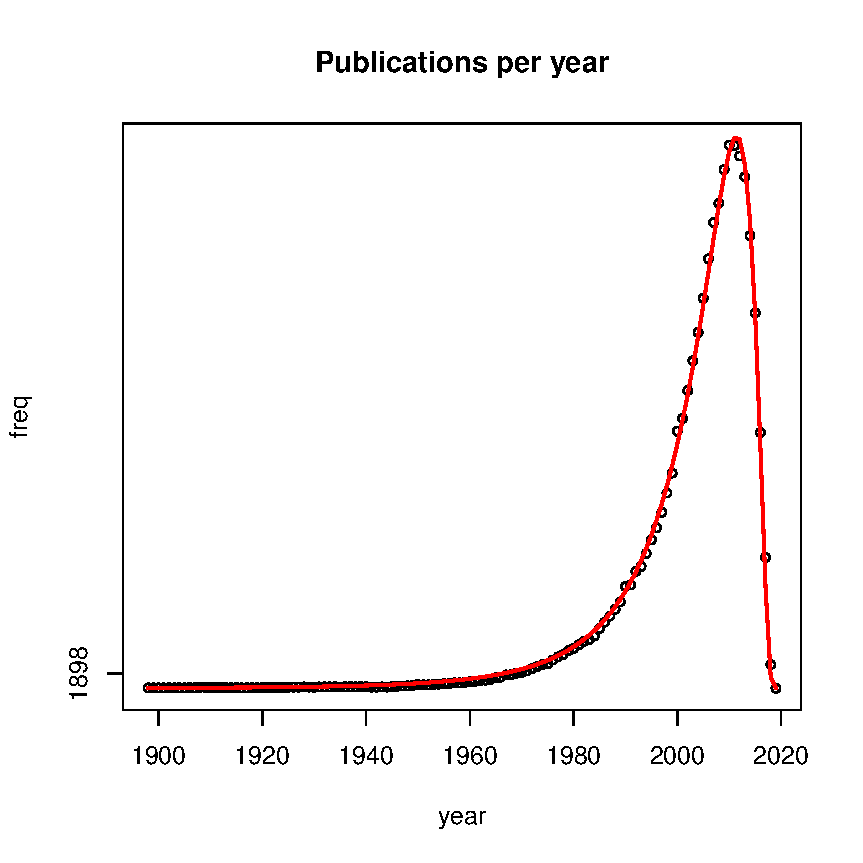
\includegraphics[width=0.45\textwidth]{pubYear.pdf} \qquad
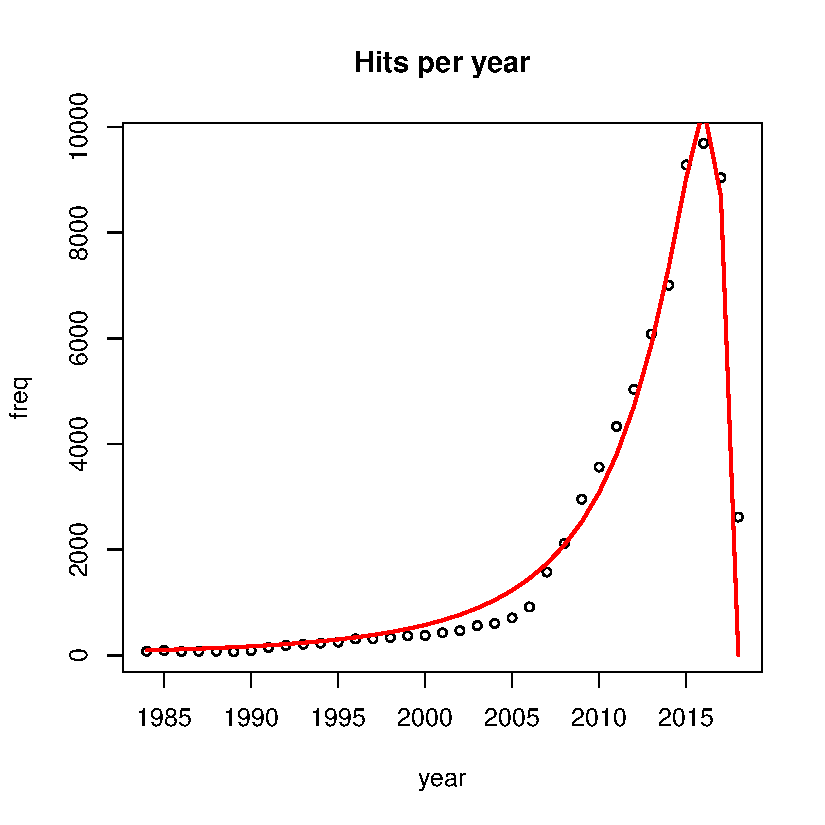
\includegraphics[width=0.45\textwidth]{yearshits7.pdf} }
\caption{Citation network: Distribution of all works and hits by years}\label{yeard}
\end{figure}
\medskip   

In the Figure~\ref{cindeg}, the indegree distribution in citation network -- cumulative and density in double-logarithmic scale  is shown. This distribution fits well the the \keyw{power law} $f = c \cdot n^{-\alpha}$, with fitted $\alpha = 2.3007$, $c=749338$, which means that the small number of works   attracts a large number of citations, and the large number of works attracts only small number of citations. Works with the largest indegrees are the most cited papers. 

\begin{figure}
\centerline{
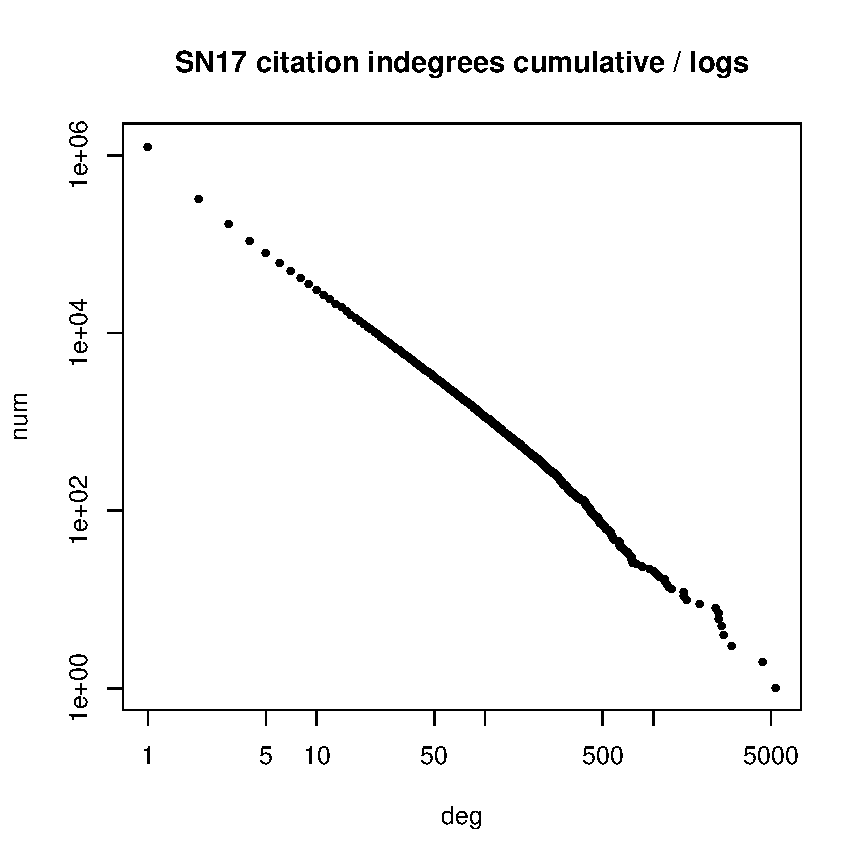
\includegraphics[width=0.45\textwidth]{CiteIndegCum.pdf} \qquad
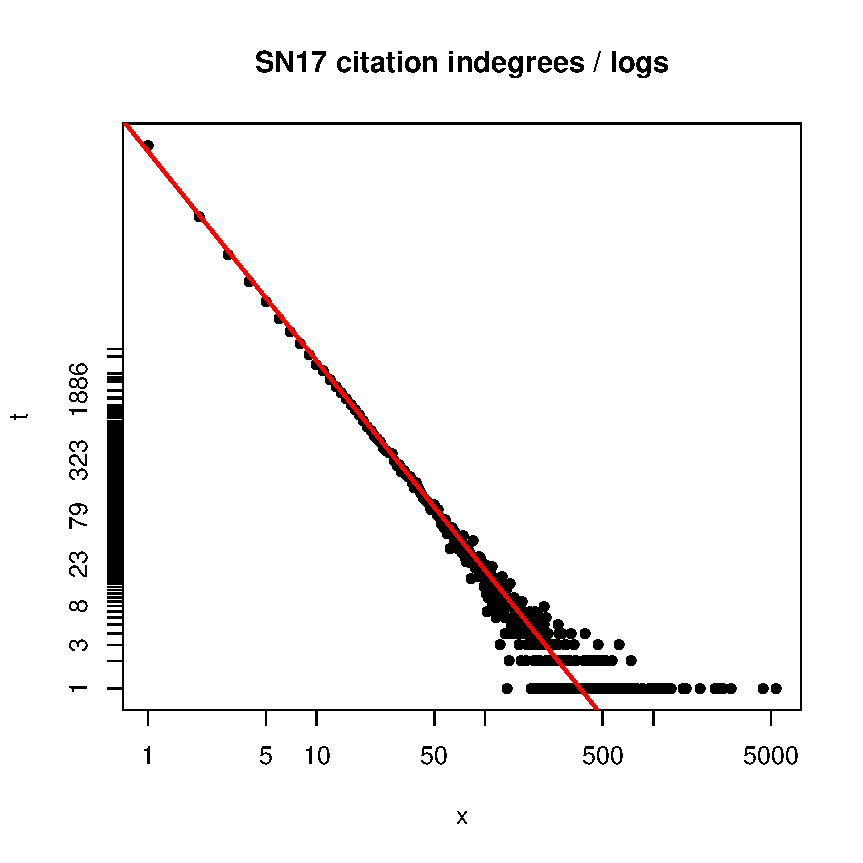
\includegraphics[width=0.45\textwidth]{CiteIndegplfit.pdf} }
\caption{Citation network: Indegree distribution}\label{cindeg}
\end{figure}
\medskip   

Table~\ref{mostcited} presents 60 the most $cited$ works (indegree in \textbf{CiteN}). Almost half -- 28 -- of these works are published earlier, before 2000, and some of them (15) are books. The top ranked work is the well-known book of Wasserman and Faust published in 1994, and the second ranked one is also a classical article of Granovetter on the ``strenght of weak ties'' concept. The other books of  ``social'' networks scientists cited more then 500 times (number in parentheses) are:  Burt RS, Structural Holes: The Social Structure of Competition, 1992 (2333); Putnam RD, Bowling alone: America’s declining social capital, 2000 (1510); Scott J, Social Network Analysis: A Handbook, 2000 (1192); Everett MG, \textit{Ucinet for Windows: Software for social network analysis}, 2002 (1171); Coleman J, Foundations of Social Theory, 1990 (1093); Borgatti SP,  \textit{Ucinet for Windows: Software for Social Network Analysis}, 2002 (999); Hanneman RA, Introduction to social network methods, 2005 (854); Lin N, Social capital. A theory of social structure and action, 2001 (800); Rogers EM, Diffusion of innovations, 2003 (628); Putnam RD, Making democracy work: Civic institutions in modern Italy, 1993 (613); Zachary WW, An information flow model for conflict and fission in small groups, 1977 (583); Burt, RS	Brokerage and closure: An introduction to social capital, 2005 (565);  Rogers EM, Diffusion of Innovation. 4th, 1995 (555);  Fischer CS, To dwell among friends: Personal networks in town and city, 1982 (539). Other artciles of ``social'' network scientists listed in the table (topics in parentheses) belong to McPherson (homophily), Freeman and Bonachich (centrality, betweenness), Burt (structural holes), Coleman, Portes, Adler (social capital), Granovetter, Uzzi (embeddedness), Milgram (small world), and Borgatti. \medskip 

Interestingly, the list also includes a lot of names of phisicists working within the network approach: highly ranked articles of Watts DJ -- Collective dynamics of 'small-world' networks, appeared in NATURE in 1998 (2906), as well as Barabasi AL --  Emergence of scaling in random networks, appeared in SCIENCE in 1999 (2614). Other works are of Newman, Albert, Girvan, Fortunato, Blondel, Clauset on large and complex networks, community detection and clustering. A famous work of Erd\H{o}s ``On random graphs'', published in 1959, is also in the list. \medskip 

There are also some representatives of the other spheres -- in such expected  topics as social network sites and social media (including highly rated article of Boyd D, Social network sites: Definition, history, and scholarship, published in 2007 and having 2447 citations); medicine (including famous works of Christakis NA on spread of obesity and smoking), and management. \medskip 

\begin{table}
\caption{Citation net:\label{mostcited} The most cited works - indegree}\medskip
\renewcommand{\arraystretch}{0.95}
%\small
\begin{tabular}{r|r|l||r|r|l}
i	& freq	& id	                                           & i	& freq & id \\ \hline
1& 	5348& 	WASSERMA\_S(1994):& 	31& 	734& 	NEWMAN\_M(2001)98:404	\\
2& 	4471& 	GRANOVET\_M(1973)78:1360& 	32& 	719& 	NEWMAN\_M(2010):	\\
3& 	2906& 	WATTS\_D(1998)393:440& 	33& 	701& 	PORTES\_A(1998)24:1	\\
4& 	2614& 	BARABASI\_A(1999)286:509& 	34& 	687& 	BLEI\_D(2003)3:993	\\
5& 	2561& 	FREEMAN\_L(1979)1:215& 	35& 	670& 	BURT\_R(2004)110:349	\\
6& 	2447& 	BOYD\_D(2007)13:210& 	36& 	654& 	HANSEN\_M(1999)44:82	\\
7& 	2429& 	MCPHERSO\_M(2001)27:415& 	37& 	639& 	PALLA\_G(2005)435:814	\\
8& 	2330& 	BURT\_R(1992):& 	38& 	634& 	CLAUSET\_A(2004)70:066111	\\
9& 	1886& 	COLEMAN\_J(1988)94:95& 	39& 	629& 	BONACICH\_P(1987)92:1170	\\
10& 	1572& 	NEWMAN\_M(2003)45:167& 	40& 	628& 	ERDOS\_P(1959)6:290	\\
11& 	1520& 	GIRVAN\_M(2002)99:7821& 	41& 	628& 	UZZI\_B(1997)42:35	\\
12& 	1510& 	PUTNAM\_R(2000):& 	42& 	628& 	ROGERS\_E(2003):	\\
13& 	1285& 	ALBERT\_R(2002)74:47& 	43& 	613& 	PUTNAM\_R(1993):	\\
14& 	1240& 	GRANOVET\_M(1985)91:481& 	44& 	593& 	BERKMAN\_L(1979)109:186	\\
15& 	1192& 	SCOTT\_J(2000):& 	45& 	583& 	ZACHARY\_W(1977)33:452	\\
16& 	1171& 	EVERETT\_M(2002):& 	46& 	572& 	BORGATTI\_S(2009)323:892	\\
17& 	1166& 	NEWMAN\_M(2004)69:026113& 	47& 	569& 	NEWMAN\_M(2001)64:025102	\\
18& 	1093& 	COLEMAN\_J(1990):& 	48& 	565& 	BURT\_R(2005):	\\
19& 	1058& 	STEINFIE\_C(2007)12:1143& 	49& 	561& 	ADLER\_P(2002)27:17	\\
20& 	1034& 	FORTUNAT\_S(2010)486:75& 	50& 	559& 	CHRISTAK\_N(2008)358:2249	\\
21& 	999& 	BORGATTI\_S(2002):& 	51& 	555& 	ROGERS\_E(1995):	\\
22& 	945& 	CHRISTAK\_N(2007)357:370& 	52& 	554& 	MILGRAM\_S(1967)1:61	\\
23& 	867& 	FREEMAN\_L(1977)40:35& 	53& 	553& 	BARON\_R(1986)51:1173	\\
24& 	854& 	HANNEMAN\_R(2005):& 	54& 	550& 	GRANOVET\_M(1978)83:1420	\\
25& 	800& 	LIN\_N(2001):& 	55& 	539& 	FISCHER\_C(1982):	\\
26& 	757& 	KAPLAN\_A(2010)53:59& 	56& 	537& 	BRIN\_S(1998)30:107	\\
27& 	756& 	BLONDEL\_V(2008):P10008& 	57& 	524& 	MARSDEN\_P(1990)16:435	\\
28& 	742& 	NAHAPIET\_J(1998)23:242& 	58& 	523& 	KEMP\_D(2003):137	\\
29& 	740& 	FORNELL\_C(1981)18:39& 	59& 	523& 	KLEINBER\_J(1999)46:604	\\
30& 	740& 	NEWMAN\_M(2006)103:8577& 	60& 	517& 	BOCCALET\_S(2006)424:175	\\ \hline
\end{tabular}
\end{table}

\Remark{remove Table 3?}
Table~\ref{maxciting} shows 20 the most \emph{citing} works (works with the largest outdegree in \textbf{CiteN}). These works are books, books introductory chapters, and review articles. Most of these works belong to the field of social sciences and cover different topics, including education, human relationships, archeology, migration, internet studies, and social media. The topic of social network analysis is not presented separately in this type of works. However, it is presented in the works published in journals in Physics and Computer Science from the list (Bocaletti on complex networks, Costa on complex networks, Castellano on social physics of social dynamics, Brandes on methodological foundations of network analysis), as well as works representing -- quite surprisingly -- the field of Animal social networks. 

\begin{table}
\caption{Citation net: \label{maxciting} The most citing work -- outdegree}
\renewcommand{\arraystretch}{0.95}
%\small
\begin{tabular}{r|r|l||r|r|l}
i&	freq& 	id&	i&	freq&	id	\\ \hline 
1& 	1572& 	CHAPMAN\_C(2016):1&	11& 	731& 	TSATSOU\_P(2014):1\\
2& 	1406& 	HRUSCHKA\_D(2010)5:1&	12& 	654& 	GOODALE\_E(2017):IX\\
3& 	1293& 	COWARD\_F(2015):1&	13& 	649& 	PEPPER\_G(2017)40:S0140525X1700190X\\
4& 	1254& 	FITZGERA\_P(2008):1&	14& 	632& 	STROM\_R(2012):1\\
5& 	1207& 	DAVIES\_N(2015):V&	15& 	613& 	SCHACHNE\_G(2015)23:49\\
6& 	1055& 	MARSH\_C(2009):1&	16& 	597& 	COSTA\_L(2011)60:329\\
7& 	942& 	YUS\_F(2011)213:1&	17& 	593& 	BRANDES\_U(2005)3418:1\\
8& 	929& 	BOCCALET\_S(2006)424:175&	18& 	586& 	ROBERTS\_J(2014):1\\
9& 	799& 	REEVES\_M(2017):1&	19& 	557& 	GUNTER\_B(2016):1\\
10& 	768& 	GROSS\_J(2007):1&	20& 	547& 	CASTELLA\_C(2009)81:591\\ \hline 
\end{tabular}
\end{table}

\subsection{Distributions on WAn}

\Remark{remove Table 4?}
Table~\ref{numpap} shows authors with the largest number of papers, which is shown by the indegree distribution of the \textbf{WAn} network. Almost all of these names (Wang, Zhang, Chen, Li, Liu, Lee, Kim, Yang, Wu), except Newman, belong to Chinese authors. However, this is the result of the well-known \href{https://en.wikipedia.org/wiki/List_of_common_Chinese_surnames}{"three Zhang, four Li"} effect: as the number of original surnames in China is relatively small, there is a high chance that different authors, having the same surname and first letter of the name, shrink together, creating ``generalized'' authors. Such problem could be overcame if we would use a special ID (such as ORCID) for each scientist (but this information is not provided in WoS). 

\begin{table}
\caption{\textbf{WAn} network: \label{numpap} Authors with the largest number of papers -- indegree}
\renewcommand{\arraystretch}{0.9}
\begin{center}
\begin{tabular}{l|l|l||l|l|l}
Rank& 	Value& 	Id& 	Rank& 	Value& 	Id\\  \hline   
1& 	1169& 	WANG\_Y& 	21& 	552& 	KIM\_H\\ 
2& 	883& 	ZHANG\_Y& 	22& 	550& 	CHEN\_J\\ 
3& 	868& 	CHEN\_Y& 	23& 	536& 	LIU\_X\\ 
4& 	847& 	LI\_Y& 	24& 	533& 	WANG\_L\\ 
5& 	838& 	WANG\_X& 	25& 	509& 	LI\_H\\ 
6& 	819& 	ZHANG\_J& 	26& 	490& 	KIM\_Y\\ 
7& 	788& 	WANG\_J& 	27& 	485& 	ZHANG\_Z\\ 
8& 	786& 	LIU\_Y& 	28& 	474& 	WANG\_Z\\ 
9& 	766& 	LEE\_J& 	29& 	471& 	WANG\_S\\ 
10& 	765& 	LEE\_S& 	30& 	471& 	CHEN\_X\\ 
11& 	749& 	LI\_J& 	31& 	471& 	\textbf{NEWMAN\_M}\\ 
12& 	708& 	LI\_X& 	32& 	462& 	CHEN\_L\\ 
13& 	696& 	CHEN\_C& 	33& 	461& 	ZHANG\_L\\ 
14& 	690& 	KIM\_J& 	34& 	450& 	YANG\_Y\\ 
15& 	620& 	WANG\_H& 	35& 	450& 	ZHANG\_H\\ 
16& 	611& 	ZHANG\_X& 	36& 	432& 	WU\_J\\ 
17& 	611& 	LIU\_J& 	37& 	431& 	LEE\_H\\ 
18& 	570& 	CHEN\_H& 	38& 	420& 	LI\_Z\\ 
19& 	557& 	KIM\_S& 	39& 	420& 	WANG\_W\\ 
20& 	554& 	WANG\_C& 	40& 	417& 	LI\_L\\ \hline  
\end{tabular}
\end{center}
\end{table}

Looking at the outdegree of \textbf{WAn} network, we get the information on the number of authors in works. This distribution is presented in the Table~\ref{numpapout}. The majority of works (95.5\%) has only one author (however, the largest part of this group are works that are cited only, having information only on the first author). Other 4\% of all the works have from 2 to 5 authors. In some works, hovever, the amount of authors is pretty high. On the Table~\ref{maxnumofauthors} we present the works which have more then 25 authors. The most ``extreme'' case is the work ``Sharing and community curation of mass spectrometry data with Global Natural Products Social Molecular Networking'', published in \textit{Nature Biotechnology} in 2016, which has 126 authors. Almost all the works from this list belong to the fields of Natural science - Medical, Health, Epidemiological, and Behavioral studies. For these fields, the inclusion of all the authors inplementing a research project to the paper is quite a frequent situation.  However, the third rated article - ``Discussion on the paper by Handcock, Raftery and Tantrum'', - published in \textit{Royal Statistical Society.Journal.Series A: Statistics in Society} collects 48 ``social'' networks scientists \Remark{remove Table 6?}.\medskip

\begin{table}
\caption{WA net: \label{numpapout} Number of authors in works -- outdegree}
\renewcommand{\arraystretch}{0.9}
\begin{center}
\begin{tabular}{l|l|l||l|l|l}
outdeg&  	Freq&  	Freq\% &  	outdeg&   Freq &	Freq\%\\ \hline   
1&  	1239496&  	95.5566&  	21&  	4&  	0.0003\\
2&  	18637&  	1.4368&  	22&  	3&  	0.0002\\
3&  	16661&  	1.2844&  	23&  	4&  	0.0003\\
4&  	10617&  	0.8185&  	24&  	2&  	0.0002\\
5&  	5759&  	0.4440&  	25&  	1&  	0.0001\\
6&  	2802&  	0.2160&  	26&  	2&  	0.0002\\
7&  	1322&  	0.1019&  	27&  	5&  	0.0004\\
8&  	686&  	0.0529&  	28&  	2&  	0.0002\\
9&  	384&  	0.0296&  	29&  	1&  	0.0001\\
10&  	247&  	0.0190&  	31&  	3&  	0.0002\\
11&  	155&  	0.0119&  	36&  	1&  	0.0001\\
12&  	90&  	0.0069&  	41&  	1&  	0.0001\\
13&  	70&  	0.0054&  	42&  	1&  	0.0001\\
14&  	54&  	0.0042&  	43&  	1&  	0.0001\\
15&  	32&  	0.0025&  	48&  	1&  	0.0001\\
16&  	12&  	0.0009&  	53&  	1&  	0.0001\\
17&  	14&  	0.0011&  	126&  	1&  	0.0001\\
18&  	9&  	0.0007&  	  & 	 & 	\\
19&  	6&  	0.0005&  	 &	 &	\\
20&  	2&  	0.0002&  	&	 &	\\ \hline
SUM &     &              &       &  1297133 & 100  \\ \hline   
\end{tabular}
\end{center}
\end{table}

\begin{longtable}{l|p{1.8cm}|p{9cm}|p{3cm}|l|}
\caption{WA net: \label{maxnumofauthors} Works with the largest number of authors}\\ 
\small
\renewcommand{\arraystretch}{0.7}
Value& First author & Title & Journal & Year \\ \hline\endhead
126&	Wang, MX&	 Sharing and community curation of mass spectrometry data with Global Natural Products Social Molecular Networking&	NAT BIOTECHNOL&	2016\\
53&	Vashisht, R&	 Crowd Sourcing a New Paradigm for Interactome Driven Drug Target Identification in Mycobacterium tuberculosis&	PLOS ONE&	2012\\
48&	Snijders, TAB&	 Discussion on the paper by Handcock, Raftery and Tantrum&	J ROY STATIST SOC SER A STAT&	2007\\
43&	Gustavsson, A&	 Cost of disorders of the brain in Europe 2010&	EUR NEUROPSYCHOPHARM&	2011\\
42&	DOLL, LS&	 Homosexually and nonhomosexually identified men who have sex with men - a behavioral-comparison&	J SEX RES&	1992\\
41&	Magliano, L&	 Family psychoeducational interventions for schizophrenia in routine settings: impact on patients' clinical status and social functioning and on relatives' burden and resources&	EPIDEMIOL PSICHIATR SOC&	2006\\
36&	Auradkar, A&	 Data Infrastructure at LinkedIn&	PROC INT CONF DATA&	2012\\
31&	Durkee, T&	 Prevalence of pathological internet use among adolescents in Europe: demographic and social factors&	ADDICTION&	2012\\
31&	Kaur, K&	 Fluoroquinolone-related neuropsychiatric and mitochondrial toxicity: a collaborative investigation by scientists and members of a social network&	J COMMUNITY SUPPORT&	2016\\
31&	Hermanussen, M&	 Adolescent Growth: Genes, hormones and the Peer Group. Proceedings of the 20th Aschauer Soiree, held at Gkicksburg castle, Germany, 15th to 17th November 2013&	PEDIATR ENDOCR REV P&	2014\\
29&	Corazza, O&	 Promoting innovation and excellence to face the rapid diffusion of Novel Psychoactive Substances in the EU: the outcomes of the ReDNet project&	HUM PSYCHOPHARM CLIN&	2013\\
28&	Magliano, L&	 "I have got something positive out of this situation'': psychological benefits of caregiving in relatives of young people with muscular dystrophy&	J NEUROL&	2014\\
28&	Console, L&	 WantEat: interacting with social networks of smart objects for sharing cultural heritage and supporting sustainability&	FRONT ARTIF INTEL AP&	2012\\
27&	Sikora, M&	 Ancient genomes show social and reproductive behavior of early Upper Paleolithic foragers&	SCIENCE&	2017\\
27&	Magliano, L&	 Burden, professional support, and social network in families of children and young adults with muscular dystrophies&	MUSCLE NERVE&	2015\\
27&	Lopez-Fernandez, O&	 Self-reported dependence on mobile phones in young adults: A European cross-cultural empirical survey&	J BEHAV ADDICT&	2017\\
27&	Gine-Garriga, M&	 The SITLESS project: exercise referral schemes enhanced by self-management strategies to battle sedentary behaviour in older adults: study protocol for a randomised controlled trial&	TRIALS&	2017\\
27&	Maher, BS&	 The AVPR1A Gene and Substance Use Disorders: Association, Replication, and Functional Evidence&	BIOL PSYCHIAT&	2011\\
26&	SEMPLE, SJ&	 Identification of psychobiological stressors among hiv-positive women&	WOMEN HEALTH&	1993\\
26&	Wang, X&	 Reliability and validity of the international dementia alliance schedule for the assessment and staging of care in China&	BMC PSYCHIATRY&	2017\\
25&	Banos, O&	 An Innovative Platform for Person-Centric Health and Wellness Support&	LECT N BIOINFORMAT&	2015\\
\end{longtable}

\subsection{Distributions on WJn}

The distributuion of number of works per journals is presented on the Figure ~\ref{worksjour}. According to the indegree distribution of the \textbf{WJn} network, the majority of jornals -- in sum, 82\% -- are represented  in the data set with 1 (57\%), 2 (12\%), 3 (6\%), 4 (4\%) or 5 (2.5\%) works. Other 18\% (12,533) journals have 6 works and more. Table~\ref{jourind} shows the most used journals, which have the maximum values of indegree distribution. In general, there are quite a lot of journals from Social sciences in the list, which are marked in boldface. The dominant journal is \textit{Lecture Notes in Computer Science}, which has more then 7,000 citations, followed by \textit{Social Science \& Medicine} and \textit{Journal of Personality and Social Psychology} with more then 3,000 citations. Other journals that have more then 2,000 citations are multidisciplinary journals \textit{Science, Proceedings of the National Academy of Sciences of the USA, Nature}, as well as  such disciplinary journals as \textit{Computers in Human Behavior, American Journal of Public Health, and American Sociological Review}. These journals are followed by other top-ranked journals in different disciplines having more than 1,500 citations, such as (descending number of citations) \textit{Physica A, Animal Behaviour, Journal of the American Medical Association, Lancet, Scientometrics, American Journal of Sociology, Academy of Management Journal, Lecture Notes in Artificial Intelligence, Journal of Applied Psychology, American Economic Review}. The main Social network analysis field`s outlet \textit{Social Networks} journal is on the19-th place. The remaining journals cover many disciplines such as  Medicine, Psychiatry, Gerontology, Epidemiology, Psychology, Management, Marketing, Computer and Information science. \medskip

\begin{figure}
\centerline{\includegraphics[width=120mm]{WorksPerJour1.pdf}}
\caption{WJn network: Distribution of number of works by journals}\label{worksjour}
\end{figure}
\medskip   

\begin{table}
\caption{WJ net:\label{jourind}The most used journals -- indegree}\medskip
\small
\renewcommand{\arraystretch}{0.95}
%\small
\begin{tabular}{c|r|l||c|r|l}
Rank&   	Value&   	Id&   	Rank&   	Value&   	Id \\ \hline
1&   	7080&   	LECT NOTES COMPUT SC&   	31&   	1258&   	RES POLICY{AM J PSYCHIAT}\\   
2&   	3859&   	SOC SCI MED&   	32&   	1221&   	J BUS RES\\   
3&   	3408&   	J PERS SOC PSYCHOL&   	33&   	1217&   	\textbf{MANAGE SCI}\\   
4&   	2719&   	COMPUT HUM BEHAV&   	34&   	1185&   	\textbf{ACAD MANAGE REV}\\   
5&   	2631&   	SCIENCE&   	35&   	1182&   	\textbf{J CONSULT CLIN PSYCH}\\   
6&   	2602&   	AM J PUBLIC HEALTH&   	36&   	1151&  \textbf {ORGAN SCI}\\   
7&   	2599&   	P NATL ACAD SCI USA&   	37&   	1150&   	ADDICTION\\   
8&   	2208&   	NATURE&   	38&   	1143&   	\textbf{STRATEGIC MANAGE J}\\   
9&   	2058&   	\textbf{AM SOCIOL REV}&   	39&   	1087&   	\textbf{J GERONTOL B-PSYCHOL}\\   
10&   	1945&   	PHYSICA A&   	40&   	1075&   	PEDIATRICS\\   
11&   	1815&   	ANIM BEHAV&   	41&   	1055&   	AM J EPIDEMIOL\\   
12&   	1778&   	JAMA-J AM MED ASSOC&   	42&   	1050&   	COMPUT EDUC\\   
13&   	1765&   	\textbf{AM J SOCIOL}&    43&   1022&   	DEV PSYCHO\\   
14&   	1763&   	LANCET&   		44&   	1022&   	\textbf{PSYCHOL BULL}\\   
15&   	1759&   	\textbf{SCIENTOMETRICS}&   	45&   	1007&   	J ADOLESCENT HEALTH\\   
16&   	1703&   	\textbf{ACAD MANAGE J}&   	46&   	997&   	\textbf{J MARKETING}\\   
17&   	1632&   	LECT NOTES ARTIF INT&   	47&   	996&   	ARCH GEN PSYCHIAT\\   
18&   	1573&   	\textbf{J APPL PSYCHOL}&   	48&   	994&   	AIDS BEHAV\\   
19&   	1551&   	\textbf{SOC NETWORKS}&   	49&   	972&   	PERS INDIV DIFFER\\   
20&   	1509&   	\textbf{AM ECON REV}&   	50&   	949&   	PERS SOC PSYCHOL B\\   
21&   	1433&   	\textbf{J MARRIAGE FAM}&   	51&   	947&   	J BUS ETHICS\\   
22&   	1400&   	BRIT MED J&   	52&   	939&   	\textbf{J MARKETING RES}\\   
23&   	1399&   	CHILD DEV&   	53&   	925&   	INFORM SCIENCES\\   
24&   	1373&   	EXPERT SYST APPL&   	54&   	916&   	\textbf{HARVARD BUS REV}\\   
25&   	1365&   	NEW ENGL J MED&   	55&   	915&   	IEEE T KNOWL DATA EN\\   
26&   	1363&   	COMMUN ACM&   	56&   	901&   	DRUG ALCOHOL DEPEN\\   
27&   	1355&   	RES POLICY&   	57&   	900&   	WORLD DEV\\   
28&   	1279&   	GERONTOLOGIST&   	58&   	899&   	AM J PREV MED\\   
29&   	1275&   	BRIT J PSYCHIAT&   	59&   	895&   	ADDICT BEHAV\\   
30&   	1271&   	\textbf{SOC FORCES}&   	60&   	893&   	\textbf{J CONSUM RES}\\  \hline
\end{tabular}

	

\end{table}

\subsection{Distributions on WKn}

For some works, the keywords are presented in the description in the special fields \texttt {DE} (Author Keywords) and \texttt {ID} (Keywords Plus). However, for some articles this information is not provided, thats is why they are constructed by \textbf{WoS2Pajek} from the titles of works. All composite keywords were split into single words, and lemmatization was used to deal with the ``word-equivalence problem''. \medskip

The majority of works in \textbf{WKn} (95\%) do not have any keywords - these are the works which do not have a complete description (DC=0). The amount of keywords for other 70,792 works varies from 1 to 84. \Remark{ Idea: loolk at moda, or average?} The most frequent keywords are presented in the Table~\ref{keyind}. We have `social' and `network' as the highest rated words, followed (with a large margin) by `analysis', which is trivial. Some frequently used words -- model, community, graph, structure, relationship, tie (marked in boldface) -- are related to network analysis, while others - datum, base, information, research, theory, algorithm, approach, pattern, effect -- to the scientific research in general. There are also words that related to some exact topics which are being studied in network analysis -- online,  networking, facebook, internet, site, web; health, behavior; support; communication; influence; innovation; trust. We should note that keywords can have different meanings in different contexts; however, their identification in differnt subgroups (of authors or works) can bring us better understading of the topic structure of the field. \medskip

\begin{table}
\caption{WK net: \label{keyind} The most used keywords -- indegree}\medskip
\renewcommand{\arraystretch}{0.9}
%\small
\begin{center}
\begin{tabular}{r|r|l||r|r|l}
Rank&  	Value&  	Id&  	Rank&  	Value&  	Id\\ \hline
1&  	51333&  	\textbf{social}&  	31&  	3485&  	\textbf{structure}\\
2&  	46191&  	\textbf{network}&  	32&  	3479&  	life\\
3&  	11751&         \textbf {analysis}&  	33&  	3444&  	risk\\
4&  	10219&  	\textbf{model}&  	34&  	3358&  	research\\
5&  	8104&  	\textbf{community}&  	35&  	3143&  	learn\\
6&  	8090&  	use&  	36&  	3116&  	influence\\
7&  	7596&  	base&  	37&  	3054&  	student\\
8&  	7439&  	information&  	38&  	3054&  	impact\\
9&  	7061&  	health&  	39&  	3049&  	perspective\\
10&  	7023&  	behavior&  	40&  	3042&  	complex\\
11&  	6745&  	online&  	41&  	3024&  	theory\\
12&  	6087&  	networking&  	42&  	2859&  	organization\\
13&  	5833&  	media&  	43&  	2828&  	\textbf{relationship}\\
14&  	5404&  	support&  	44&  	2802&  	algorithm\\
15&  	5101&  	communication&  	45&  	2776&  	education\\
16&  	5013&  	study&  	46&  	2714&  	group\\
17&  	4759&  	datum&  	47&  	2704&  	mobile\\
18&  	4376&  	management&  	48&  	2698&  	\textbf{tie}\\
19&  	4372&  	internet&  	49&  	2695&  	adult\\
20&  	4164&  	knowledge&  	50&  	2633&  	approach\\
21&  	4126&  	user&  	51&  	2608&  	care\\
22&  	4023&  	facebook&  	52&  	2551&  	adolescent\\
23&  	3984&  	technology&  	53&  	2479&  	role\\
24&  	3907&  	site&  	54&  	2472&  	state\\
25&  	3888&  	web&  	55&  	2467&  	innovation\\
26&  	3855&  	self&  	56&  	2434&  	pattern\\
27&  	3784&  	\textbf{graph}&  	57&  	2385&  	effect\\
28&  	3676&  	performance&  	58&  	2339&  	people\\
29&  	3534&  	service&  	59&  	2333&  	trust\\
30&  	3512&  	dynamics&  	60&  	2332&  	family\\ \hline
\end{tabular}
\end{center}

\end{table}

%******************************************************************************
\section{Topic structure of the field}  

We already presented the most common keywords in the  Table~\ref{keyind}. In this section we present the results of keywords co-occurence in different articles.  \medskip

\subsection{Network KKn production}

To construct the one-mode network \textbf{KKn}, we applied the Newman normalization  to the \textbf{reduced WKr net}: the weight of each arc [w, k] was divided by the sum of weights of all arcs having the same initial node as this arc (outdegree of a node) subtracting the initial node (article), equal to 1. Then the normalized network was transposed and multiplied with normalized network. In the obtained network, the loops were deleted and bidirected arcts were transformed to edges (with summation of the line weights). The obtained network KKn consists of 32,409 nodes and 2,799,530 edges. \medskip

\texttt{KKn = t(n(WK))*n(WK), where n(W,K)[w,k] = WK[w,k]/ (outdeg(w)-1)} \medskip

\subsection{Networks of key words co-occurence}

Exploratory analysis showed that in the obtained network, the most frequentlty words \textit{social}, \textit{network}, and \textit{analysis} were connecting most of the other keywords, that`s why we deleted these 3 nodes from the obtained network. Using Islands approach, we tried to obtain subnetwork with the size minimum 2 and maximum 75 nodes. We got a large number of islands -- 342, -- where the majority of islands (301) represent just pairs of keywords. The main island includes 75 nodes; there are also some islands of smaller sizes. \medskip

Large part of the Main island (Figure~\ref{kkmain}) are the keywords on the topic of networking sites and social media (such as \textit{networking, media, online, site, facebook, internet, technology, web 2.0}). Other central nodes are \textit{information} associated with networking topic,  words \textit{diffusion} and \textit{privacy}, as well as \textit{base} and \textit{datum} (which also have links to many other keywords, including \textit{big}, and \textit{mining}). Other two central keywords are \textit{model} and \textit{graph}, which are connected to each other and other nodes, such as \textit{dynamics, complex, spread, influence} (for the first one) and \textit{random, theory, centrality -- betweenness, large -- scale -- free, cluster} (for the second). These central nodes are also connected to the words \textit{community} and \textit{algorithm}, which have links to \textit{detection} and \textit{structure}. Other topics appeared in this subnetwork are associated with \textit{health} and \textit{education}. \medskip

\begin{figure}
\begin{center}
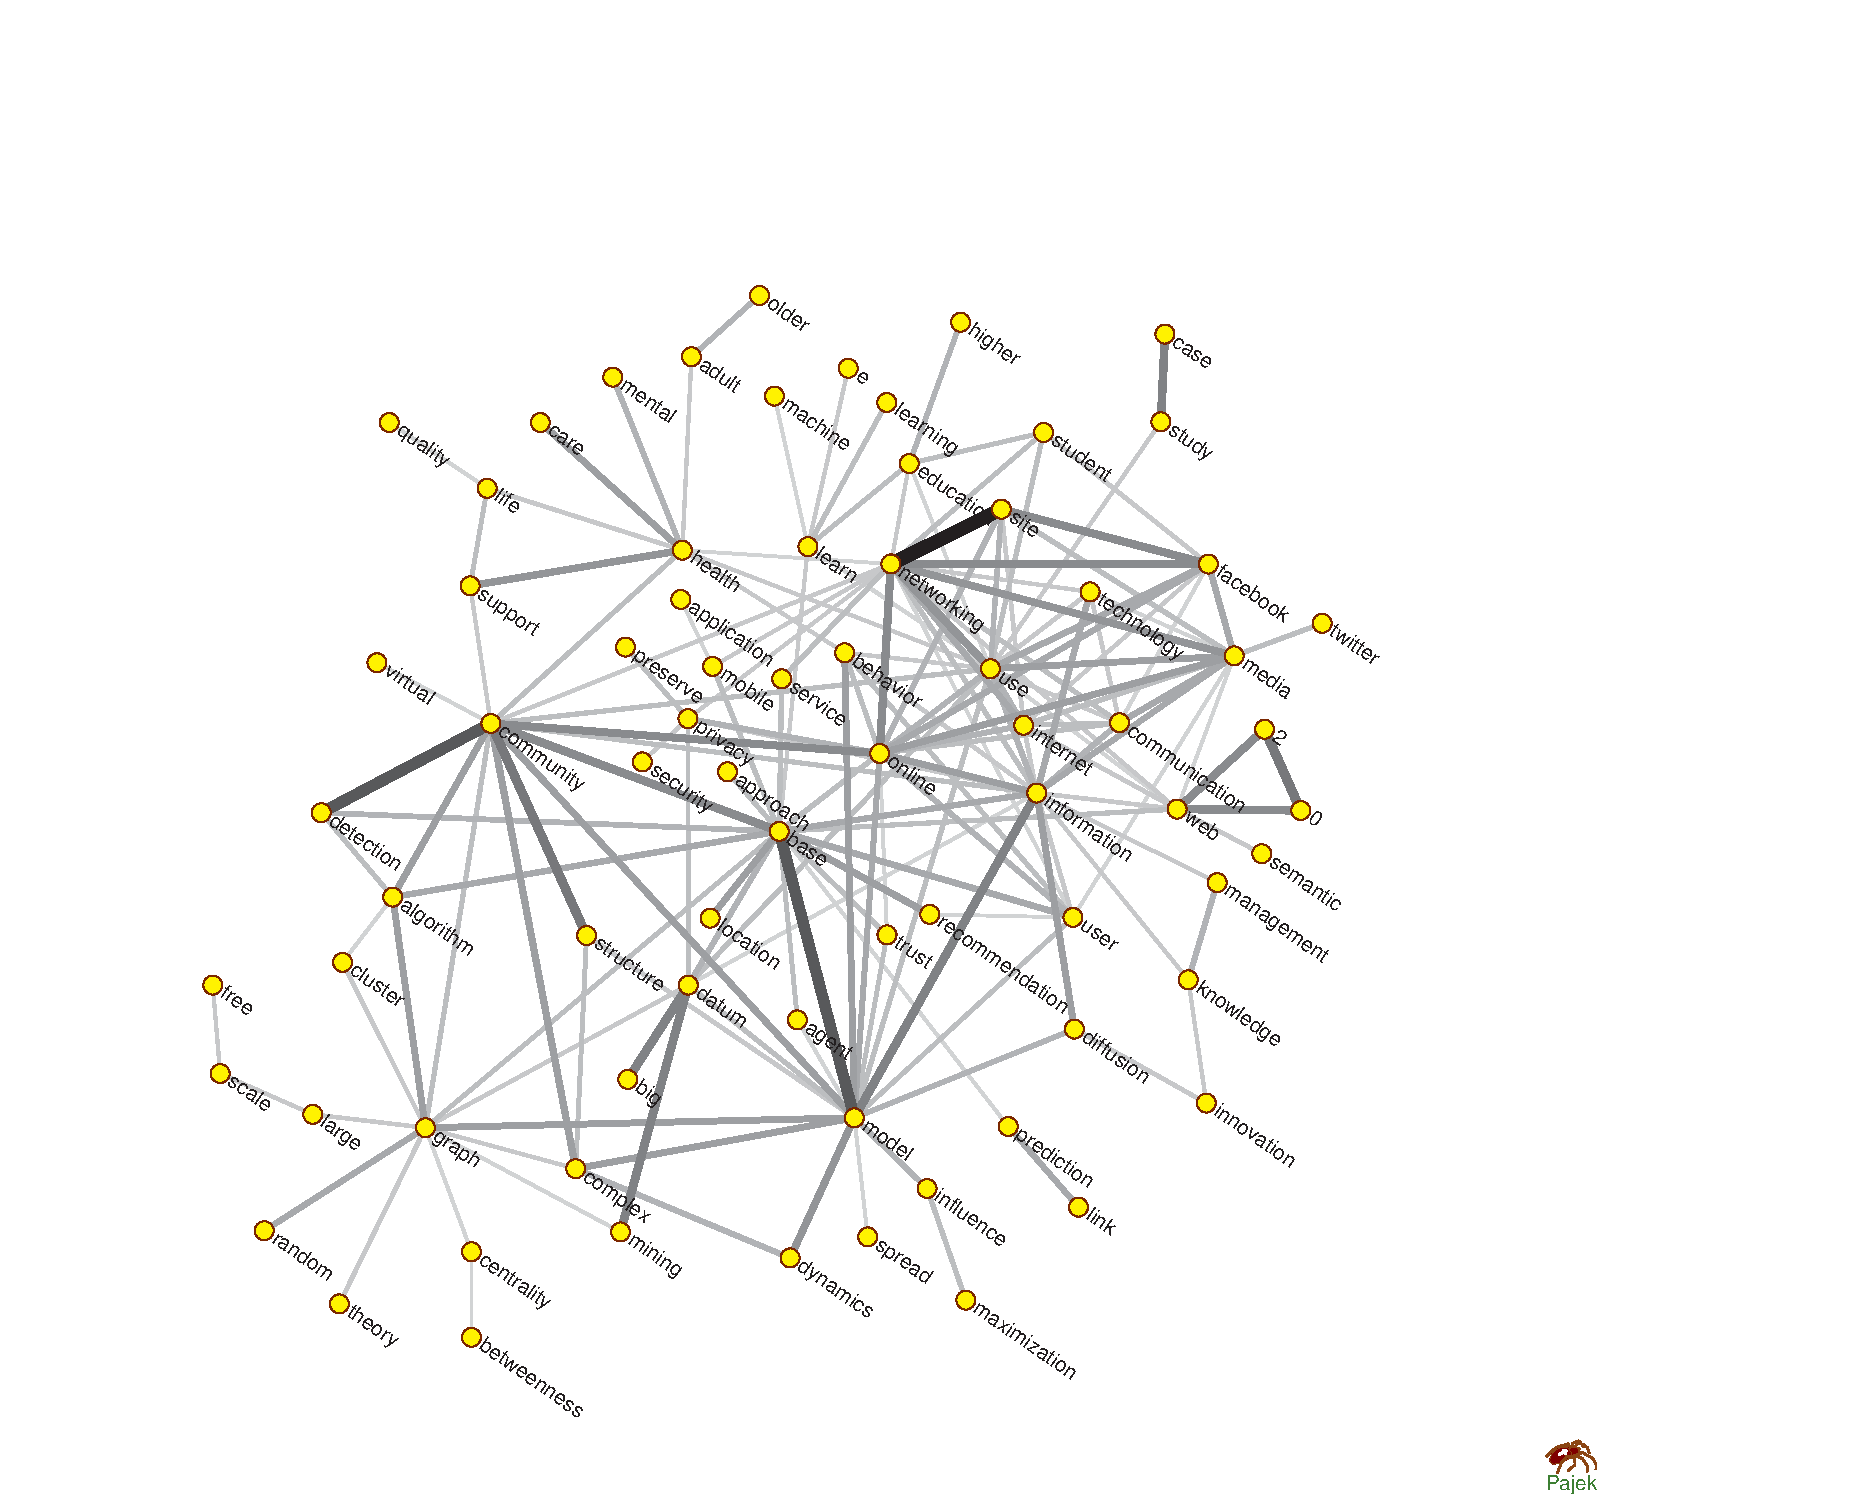
\includegraphics[width=\textwidth,viewport=93 35 665 585,clip=]{KKmain.pdf}
\end{center}
\caption{KK network Main Island} \label{kkmain}
\end{figure}

Other islands (largest are represented at the Figure~\ref{kkmid}\Remark{Probably, we do not need the Pic? Not much sense} identify some topics being studied in network analysis (\textit{strength, weak, tie; corporate - interlock - directorate; triadic - closure; small - world}, or some broade topics under study (\textit{organ - donor - donation; persecutory - delusion - paranoia; trade - international - migration}), as well as some stable phrases (\textit{special, issue, introduction}).\medskip


\begin{figure}
\begin{center}
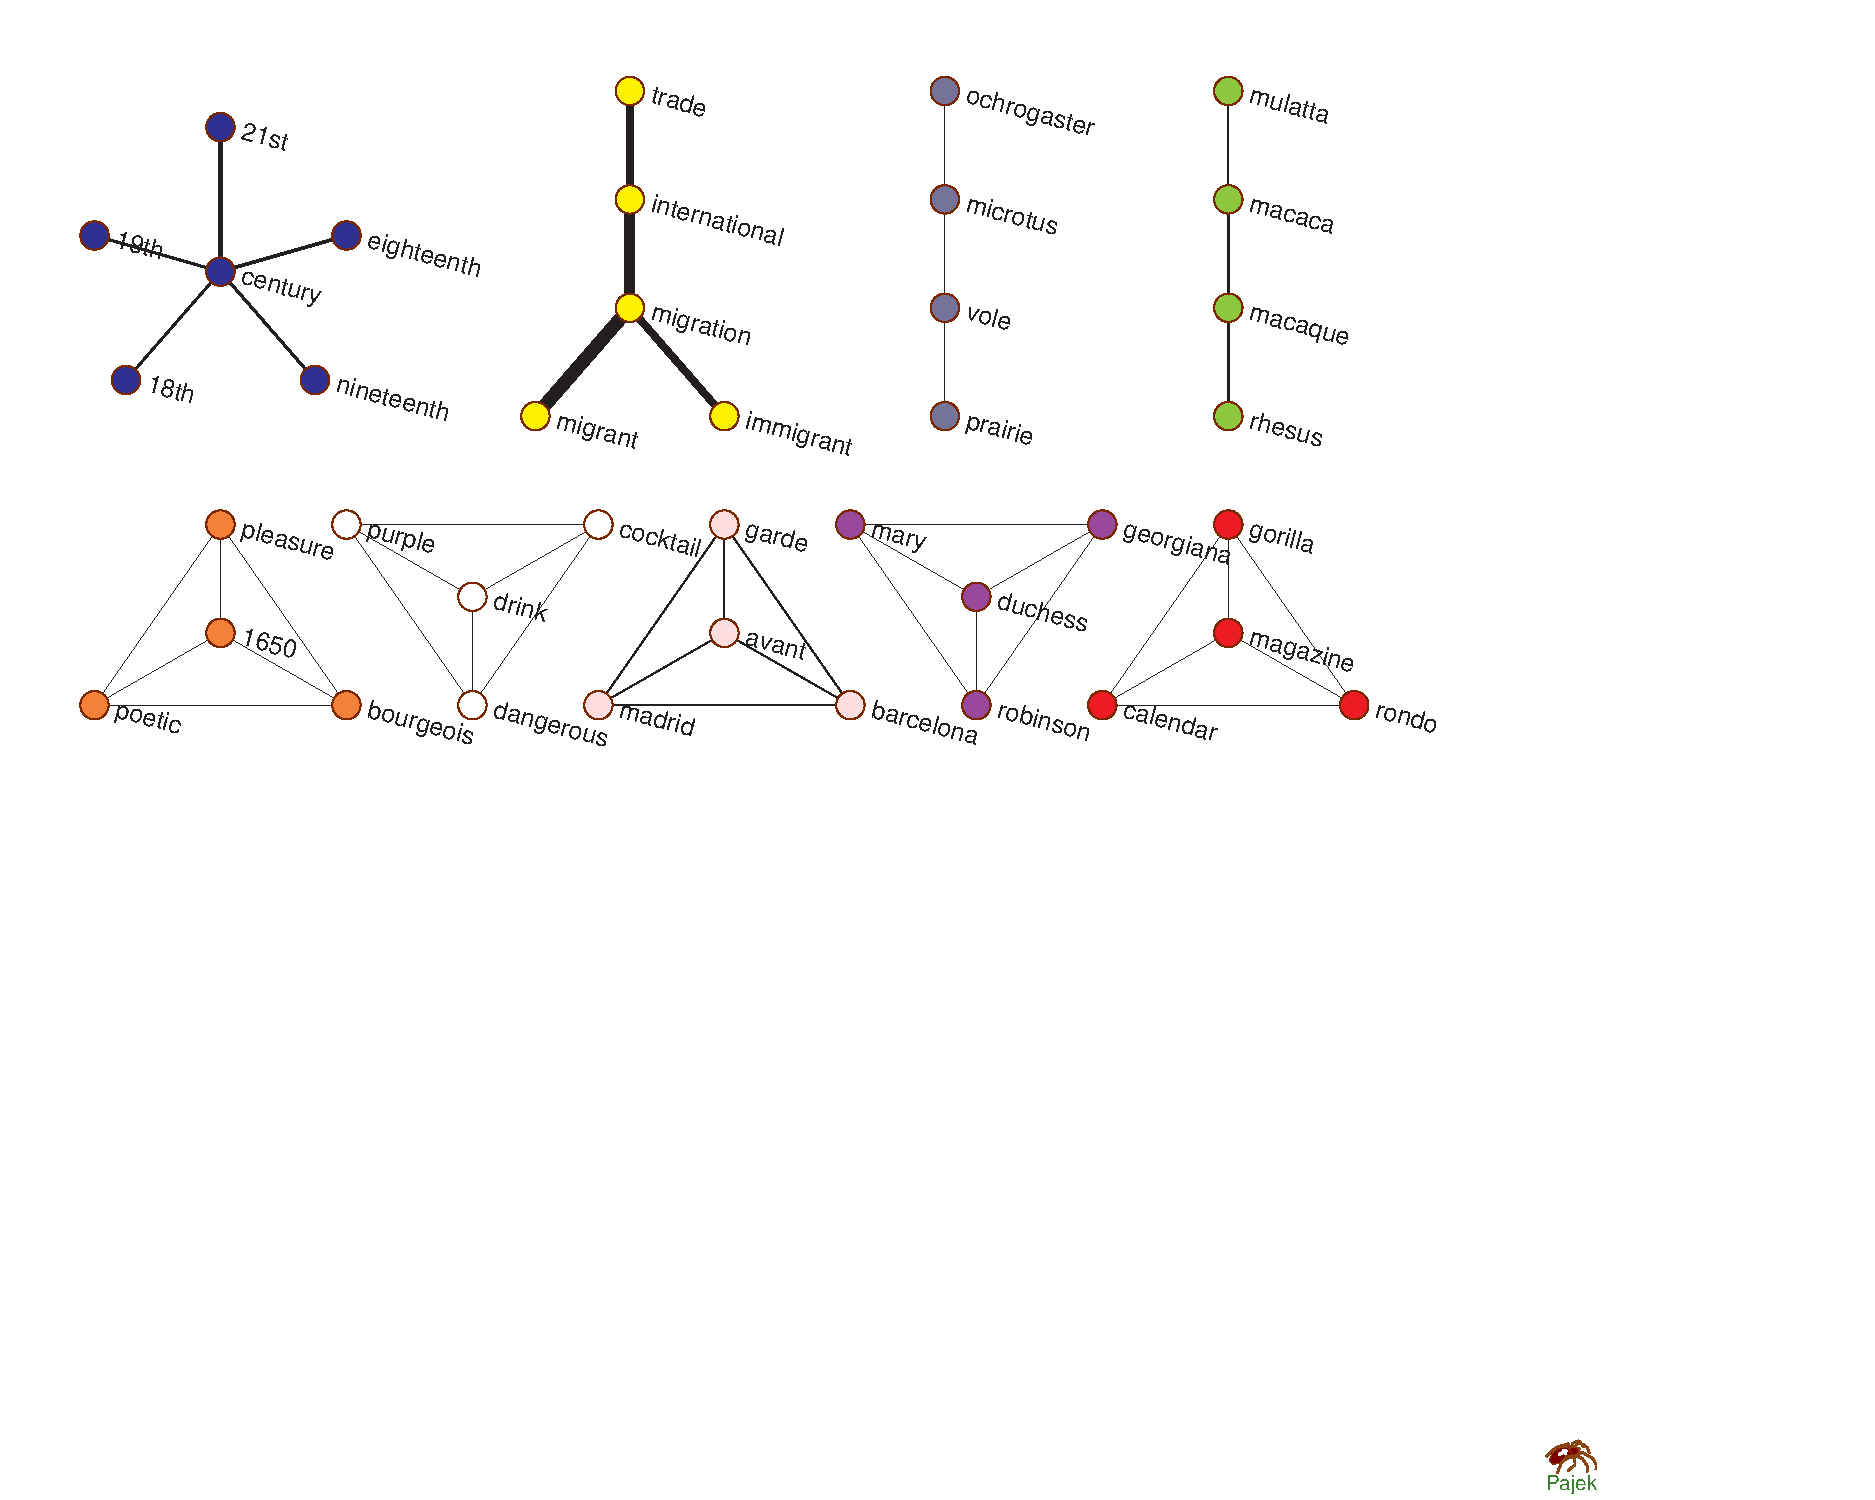
\includegraphics[width=\textwidth,viewport=35 356 695 686,clip=]{KKmid.pdf}
\end{center}
\caption{KK network Medium size Islands} \label{kkmid}
\end{figure}

%******************************************************************************
\section{Citation network}  

We restricted the original citation network \textbf{CiteN} to its `boundary' -- \textbf{CiteB} with 222,086 nodes and 1,521,434 arcs. A citation network is usually (almost) acyclic; however, it can include some small cyclic parts, which can be obtained as strong components of the network (with the minimum size 2). At first we searched for nontrivial strong components.To get an acyclic network we applied the \keyw{preprint transformation} to CiteB. The preprint transformation function replaces each work u from a strong component by pair of nodes -- published work u and its preprint version u`. Published work could cite only preprints. Each strong component was replaced by a corresponding complete bipartite graph on pairs \citep{Understand}. The resulting network \textbf{CiteT} had 222,189 nodes and 1,521,658 arcs. The increase in the number of works is due to some of them appearing twice with one name starting with an $=$ sign indicating the “preprint” version of a paper.\medskip

Then we computed the \textbf{SPC weights} on \textbf{CiteT} network arcs. The total flow is [xx] \Remark{write total flow}. We identified main paths (CPM main path and Key-route paths) in this network, and then used an \textit{Link islands approach} \citep{Understand} to find the most connected components of this network. For the same network, we also computed the \textbf{probabilistic flow}, and used the \textit{Vertex islands approach} to get its components. The obtained results are presented in the following section. \medskip

\subsection{Strong components}  

The citation network \textbf{CiteB} has 41 nontrivial strong components of different sizes, which are presented in the  Figure~\ref{citecomp}. The reciprocal (cycle) links are marked with the bluse colour, while directed pink lines also show the connections of these nodes with others. In the majority of cases, mutual referencing between the works is a characteristic of papers published in the same issue of the journal. For example, the first large cycle is combined of 12 works published in a special issue named \textit{Social Networks: new perspectives} in the journal \textit{Behavioral Ecology and Sociobiology} (Volume 63, Issue 7, May 2009). Another example are the works \texttt {BATAGELJ\_V(1992)14:63} and \texttt {BATAGELJ\_V(1992)14:121}, and \texttt {FAUST\_K(1992)14:5} and \texttt {ANDERSON\_C(1992)14:137} in the special issue on \textit{Blockmodels} in the journal \textit{Social networks} (Volume 14, Issues 1–2, March–June 1992). \medskip

Other cases are: \texttt {TUMMINEL\_M(2011):P01019} and \texttt {TUMMINEL\_M(2011)6:0017994}, \texttt{WILSON\_A(2015)69:1617} and \texttt{WILSON\_A(2015)26:1577}, \texttt { PARSEGOV\_S(2015):3475} and \texttt {PARSEGOV\_S(2017)62:2270} (same author); \texttt {VEENSTRA\_R(2013)23:399} and \texttt {DAHL\_V(2014)24:399} (same journal); \texttt {ALMAHMOU\_E(2015)33:152} and \texttt {MOK\_K(2017)35:463}, \texttt {XIA\_W(2016)3:46} and \texttt {PROSKURN\_A(2016)61:1524} (different authors and journals). \Remark{How to change these style?} \medskip

\begin{figure}
\begin{center}
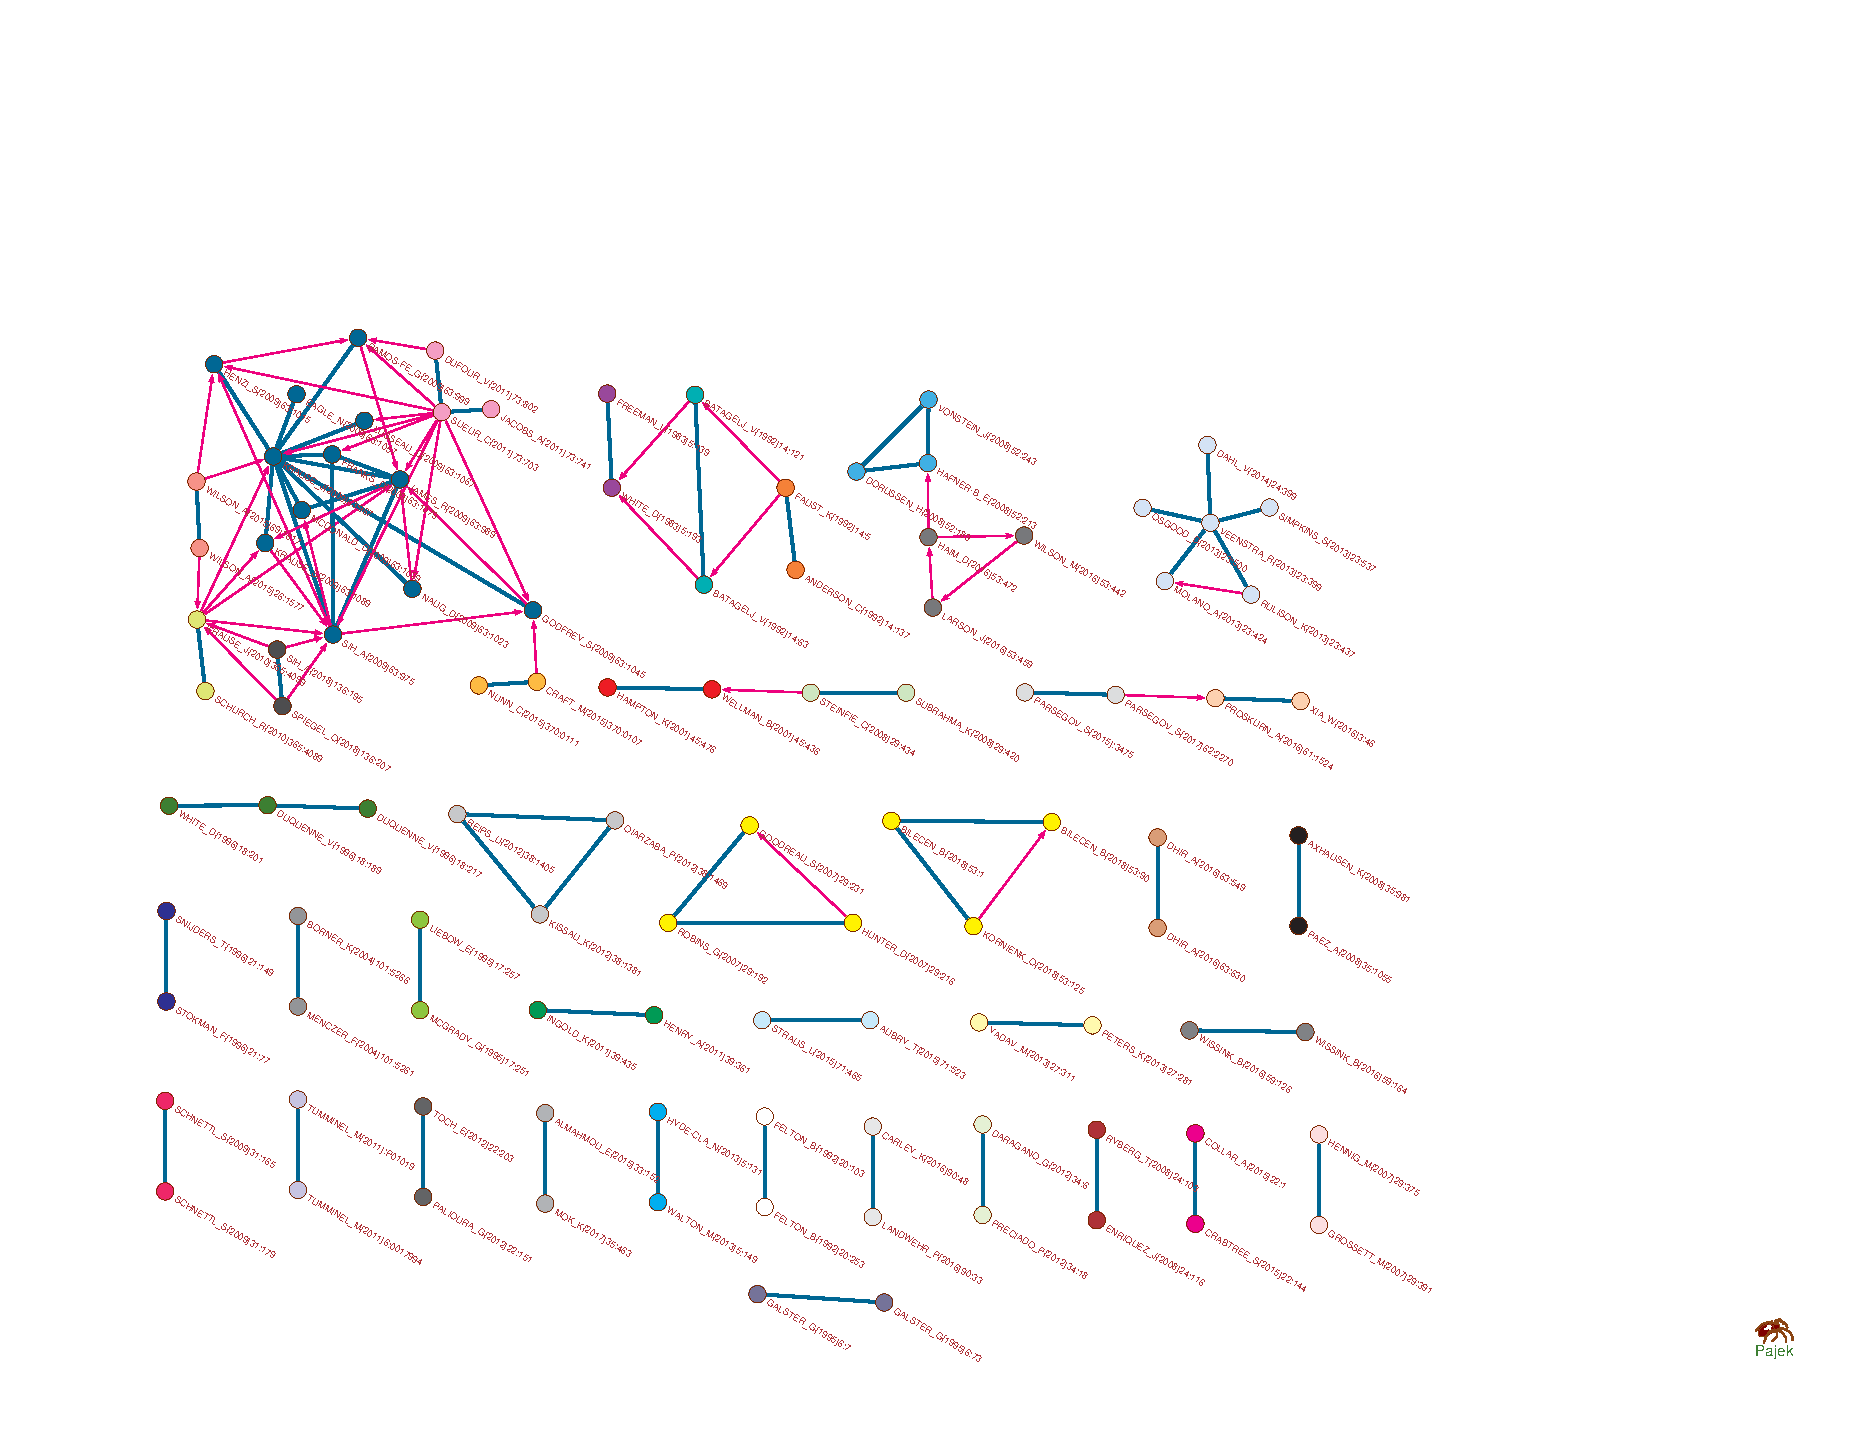
\includegraphics[width=\textwidth,viewport=75 34 690 535,clip=]{strong.pdf}
\end{center}
\caption{Strong components  \normalsize from SPC network} \label{citecomp}
\end{figure}

\subsection{CPM main path and Key Routes}  

Figure~\ref{mainFrag} shows the CPM Main path through the Social network analysis literature (which is the same to the one obtained with Main path procedure), which includes 59 nodes. We devided this CPM Main path to three parts, according to the disciplinary of the works that are presented. The first group, composed of the works published in 1944 -- 1996, present the works of `social' network scientists. These works appeared in such journals as \textit{Social networks, Administrative Science Quarterly, Annual Review of Sociology, American Sociological Review, Social Forces, Sociological Methods \& Research, Journal of Mathematical Psychology, Psychological Review, The Journal of Psychology}, recalling the history of Social network analysis field formation. In this group, 6 of 20 works belong to R. Burt. \medskip 

However, since 1999 the initiative in the field goes to the physicists, whose works appears in such journals  as \textit{Physical Review E, Journal of Statistical Physics, Reviews of Modern Physics, European Physical Journal B, Physics Reports, Nature}, and \textit{SIAM Review}. In this part of network, 9 of 14 works belong to M. Newman. \medskip 

The third part of the Main path, which contains works from 2008 to 2018, is devoted to completely another topic -- Animal social networks. The works appear at such journals as \textit{Animal Behaviour, American Journal of Primatology, Primates, Journal of Evolutionary Biology, Journal of Animal Ecology, Journal of Evolutionary Biology, Trends in Ecology \& Evolution}, and others. The most active author in this group is D. Farine, who has 6 out of 25 works.  \medskip 

While the ``invasion of physics'' into the Social network analysis field was already shown in other studies \citep{lazer,brandes}, the appearance of the third group in the Main path is quite surprising, because previously it was shown that the trend goes from Physics to Neuroscience \citep{Understand}. \medskip  

\begin{figure}
\begin{center}

\includegraphics[width=0.3\textwidth,viewport=118   28 235 262,clip=]{CPMpath.pdf}\qquad

\includegraphics[width=0.3\textwidth,viewport=118 239 235 416,clip=]{CPMpath.pdf}\qquad

\includegraphics[width=0.3\textwidth,viewport=118 394 235 681,clip=]{CPMpath.pdf}
\end{center}
\caption{Main path by fragments -- sociology, physics, biology}\label{mainFrag}
\end{figure}

The procedure of Key-route paths \citep{Understand} produces a more nuanced image of most important paths in the Social network analysis literature, as it  implies some deviations from the structure of the network, identified with the CPM Main path method.  Figure~\ref{keyRoute} shows the obtained Key-route paths, which contain 127 nodes. Basically, we can see the division into three previously mentioned groups. \medskip   

\textbf{The first period (1944--1999)} includes 50 works of the Social network analysis discipline`s representatives. It starts with two works of Heider on his theory of social perception and cognitive organization of 1944 and 1946, which form the basis for the work of Cartwright of 1956 on structural balance. Then, with some marin, two works of Holland on structural models follows, published in 1970--1971. Next comes a classical paper of Granovetter on strength of weak ties (1973), which is a basis for the works of Breiger on clustering relational data and White on blockmodels, followed by the one by Alba on the measure based on social proximity in networks, and Boorman on role structures in multiple networks, published in 1975--76. Then there are 6 works of Burt on the `main' path on the topics of positions in multiple networks (stratifiction and prestige), structural equivalence and networks subgoups, published from 1977 to 1981, which also have connections to  the works of Holland on social structure, Breiger, Lauman, and Wellman on communities structures, Breiger on social roles, and Faust on structural and general equivalences, published at about the same time period. Summing up, this group of works is dealing with network and community strcutures, positions, structural equivalence, and blockmodels.  \medskip 

These works are followed by works on measurement and different network metrics -- of Romney and Bernard (1982) on recalled data for networks constructin, and Stephenson on centrality (1989). The last work is also connected to the works of Mizruchi on measures of influence, Bonacich on power and centrality measures, and Burt, Mariolis, Mizruchi on interlock networks. This is followed by the work of Freeman on the measure of centrality, which was published in 1991, and it is very strongly connected to the work of Valente on social network thresholds in the diffusion of innovations (1996). Another strong connection of Valente goes to the previous work of Michaelson (1993) on the development of a scientific speciality as a diffusion through social relations.  \medskip 

The work of Valente is the one bridging the first group of `social' network scientists with the group of physicists, which includes 28 works from the Network science discipline and form the \textbf{second period (1999--2008)}. It is cited by Newman in the work on the small-world network model, appeared in 1999. This work is followed by others on the same topic (small-world networks), written by Moore, Newman, as well as by the work of Callaway on random graphs (2000). Then both directions meet at the work of Strogatz on complex networks, and then this topic continues, including 
clustering and preferential attachment in growing networks and spread of epidemic diseases on networks (Newman, 2001, 2002). Since 2003 to 2006, the topic went to the direction of community structures identification in large networks. \medskip 
 
We should note, however, that there is also a `epidemiological turn' in the observed network, which starts from the works of Stephens and Freeman, followed by Milardo, Neaigus, and Rothenberg in the works on the deseases transmission (1992--98), and Potterat in the infections transmission (1999). These works are cited by Ferguson (desease transmission), and then the route comes back to the main path - the Newman`s work on the structure and function of complex networks (2003). \medskip 

 Since that time, the topics of the obtained Key-routes network change significantly. The work of Newman on community stractures is strongly connected to the work of Lusseau (2009) on animal social networks, which starts the \textbf{third period (2008--2018)}, which includes 49 works of the behavioural ecologists. This work is followed by many others, at the same topic -- Krause, James (2009) with general works on Animal social network analysis, and Ramos-Fernandez, Kasper, Voell, Lehmann, Brent, Sueur (2009--2011), working with social networks of Nonhuman Primates (monkeys, baboons). These works are followed by the one of Croft (2011), which represent a practical guide on  hypothesis testing in Animal social networks. This work is cited by others presenting the research on mixed-species groups (Farine), killer whales (Foster), sharks (Mourier), dolphins (Cantor), published in 2012, and birds (Silk) and starlings (Boogert), published in 2014. There are also some more works on the methodological issues -- of Hobson ( `An analytical framework for quantifying and testing patterns of temporal dynamics in social networks'), Castels (`Social networks created with different techniques are not comparable'), and Pinter-Wollman (`The dynamics of animal social networks: analytical, conceptual, and theoretical advances'), published in 2013-2014. These works are followed by four works of Farine, published in 2015, on both methodological issues on constructing, conducting and interpreting animal social network analysis, and study of the wild birds territory acquisition. We should also note that there are some works connected to the `main' path, which represents the social personality and phenotypic types (Wilson, Alpin, Farine), published in 2013-14.\medskip   
 
The upper part of the network contains works published in the last years, 2016--18. It presents studies on desease transmission (Adelman, Sah, Silk, Dougherty), and the studies of animal paths tracking (Leu, Spiegel). Also it contains works on theoretical issues (`Current directions in animal social networks' by Croft, `Social traits, social networks and evolutionary biology' by Fisher) and implementation of different models of network analysis to Animal behaviour research:  exponential random graph models and statistical network models (Silk), the potential of stochastic actor-oriented models (Fisher),  dynamic vs. static social network analysis (Farine). \medskip   

The full information on the papers (label of the work, first author, title, journal, year of publication) included into the Main path and Key-route paths is presented on the Table~\ref{compareA}. It is also relevant for our analysis on the islands, presented in the following subsections. In this table, the second column (code) describes in which analysis the work appeared (1- Key-routes, 2- Main Path (CPM), 3- Island 5, 4 - Island 4, 5 - Node Island, 6 - Probilistic Flow Island). 
 
\begin{figure}
\begin{center}
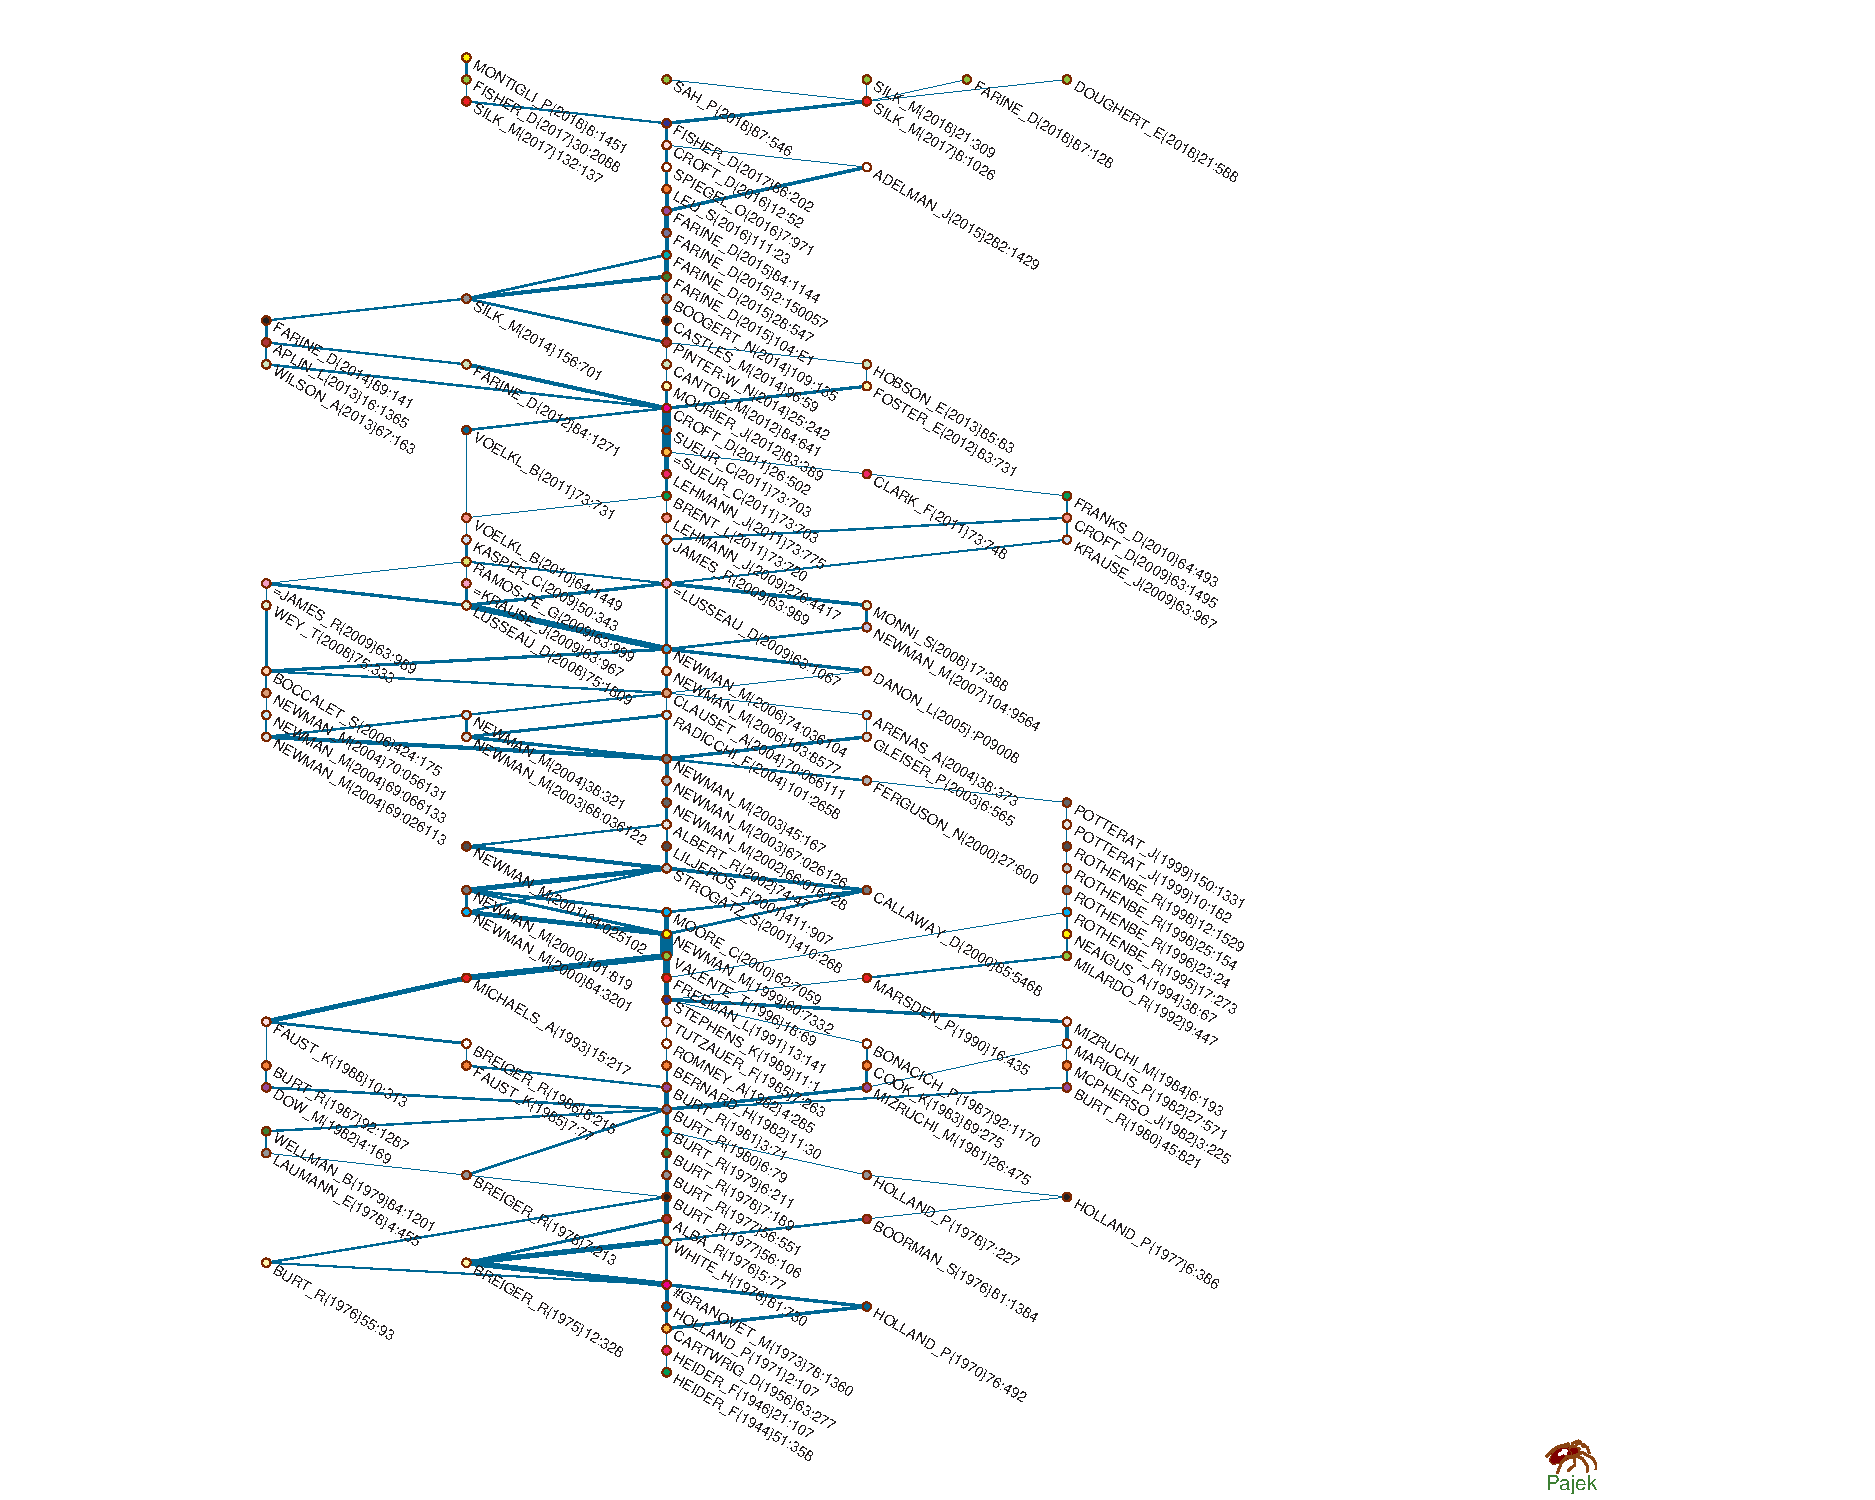
\includegraphics[width=\textwidth,viewport=120 15 605 700,clip=]{KeyRouteWxy.pdf}
\end{center}
\caption{Key Routes} \label{keyRoute}
\end{figure}

\subsection{Link Islands}

Using Islands approach, we searched for SPC link islands (on line weights) with the number of nodes between 20 and 200, and found 5 islands of 138, 65, 13, 12, and 11 nodes. The obtained largest Islands 4 of 138 nodes is presented on the Figure~\ref{island4}. Its structure reminds the structure of the Key-route paths - there are 89 overlapping nodes in two networks. The majority of the works presented in this island (from bottom to the work of Valente, published in 1996) belong to the `social' network scientists, whose works were alreday discussed upper. In comparison to the Key-routes, this network includes more evident group of works on blockmodeling - by Faust, Doreian, and Batagelj, published in 1992--1997. In the `physicists' part (from Newman, 1999 to Newman, 2006 on the `main' route) the topic of evolving networks is also presented (Bianconi, Yook, 2001, Jeong, 2003). The third, behavioural ecologists` part is pretty short and finishes by the works on Animal social networks published in 2010.  \medskip   

However, this group is fully presented in another Island 5 containing 65 nodes and presented on the Figure~\ref{island4}. It has 39 overlapping nodes with the Key-routes. `New' works presented in the island also belong to the topics on Animal social networks described above. Howver, there are some more works devoted to the methodological issues of Network analysis itself --  reconstructing animal social networks from independent small-group observations (Perreault, 2010), temporal dynamics and network analysis (Blonder, 2012), mining of animal social systems (Krause, 2013), animal social network inference and permutations for ecologists in R  (Farine, 2013), estimating uncertainty and reliability of social network data using Bayesian inference (Farine, 2015). It is ineteresting that this group form a separate subnetwork, even though it is connected to the upper part of Island 4 by topic. It may mean that the works included into this subnetwork are more connected to each other, while social animal network works in the Island 4 are more stongly connected to the works of phisicists.  \medskip   

Three other obtained islands are presented on the Figure~\ref{citeisl1-3}. For the purpose of better visibility of the picture, the weights were maximized by 100. The left Island 2 consitst of 12 work in the field of social networks in educations, imcluding issues of leadership, teachers and students communication and collaboration. Another very coherent group is presented in the same figure on the bottom left. These are 11 works in Neuropsychiatrie written bu Austrian authors. The left upper island presenets 13 works of physicists with the strongest links between the work of Bocaletti published in 2014 on the structure and dynamics of multilayer networks and others on the topics of complex, multilayer, dynamic, and temporal networks, as well as spreading processes in these networks.  \medskip    

\begin{figure}
\begin{center}
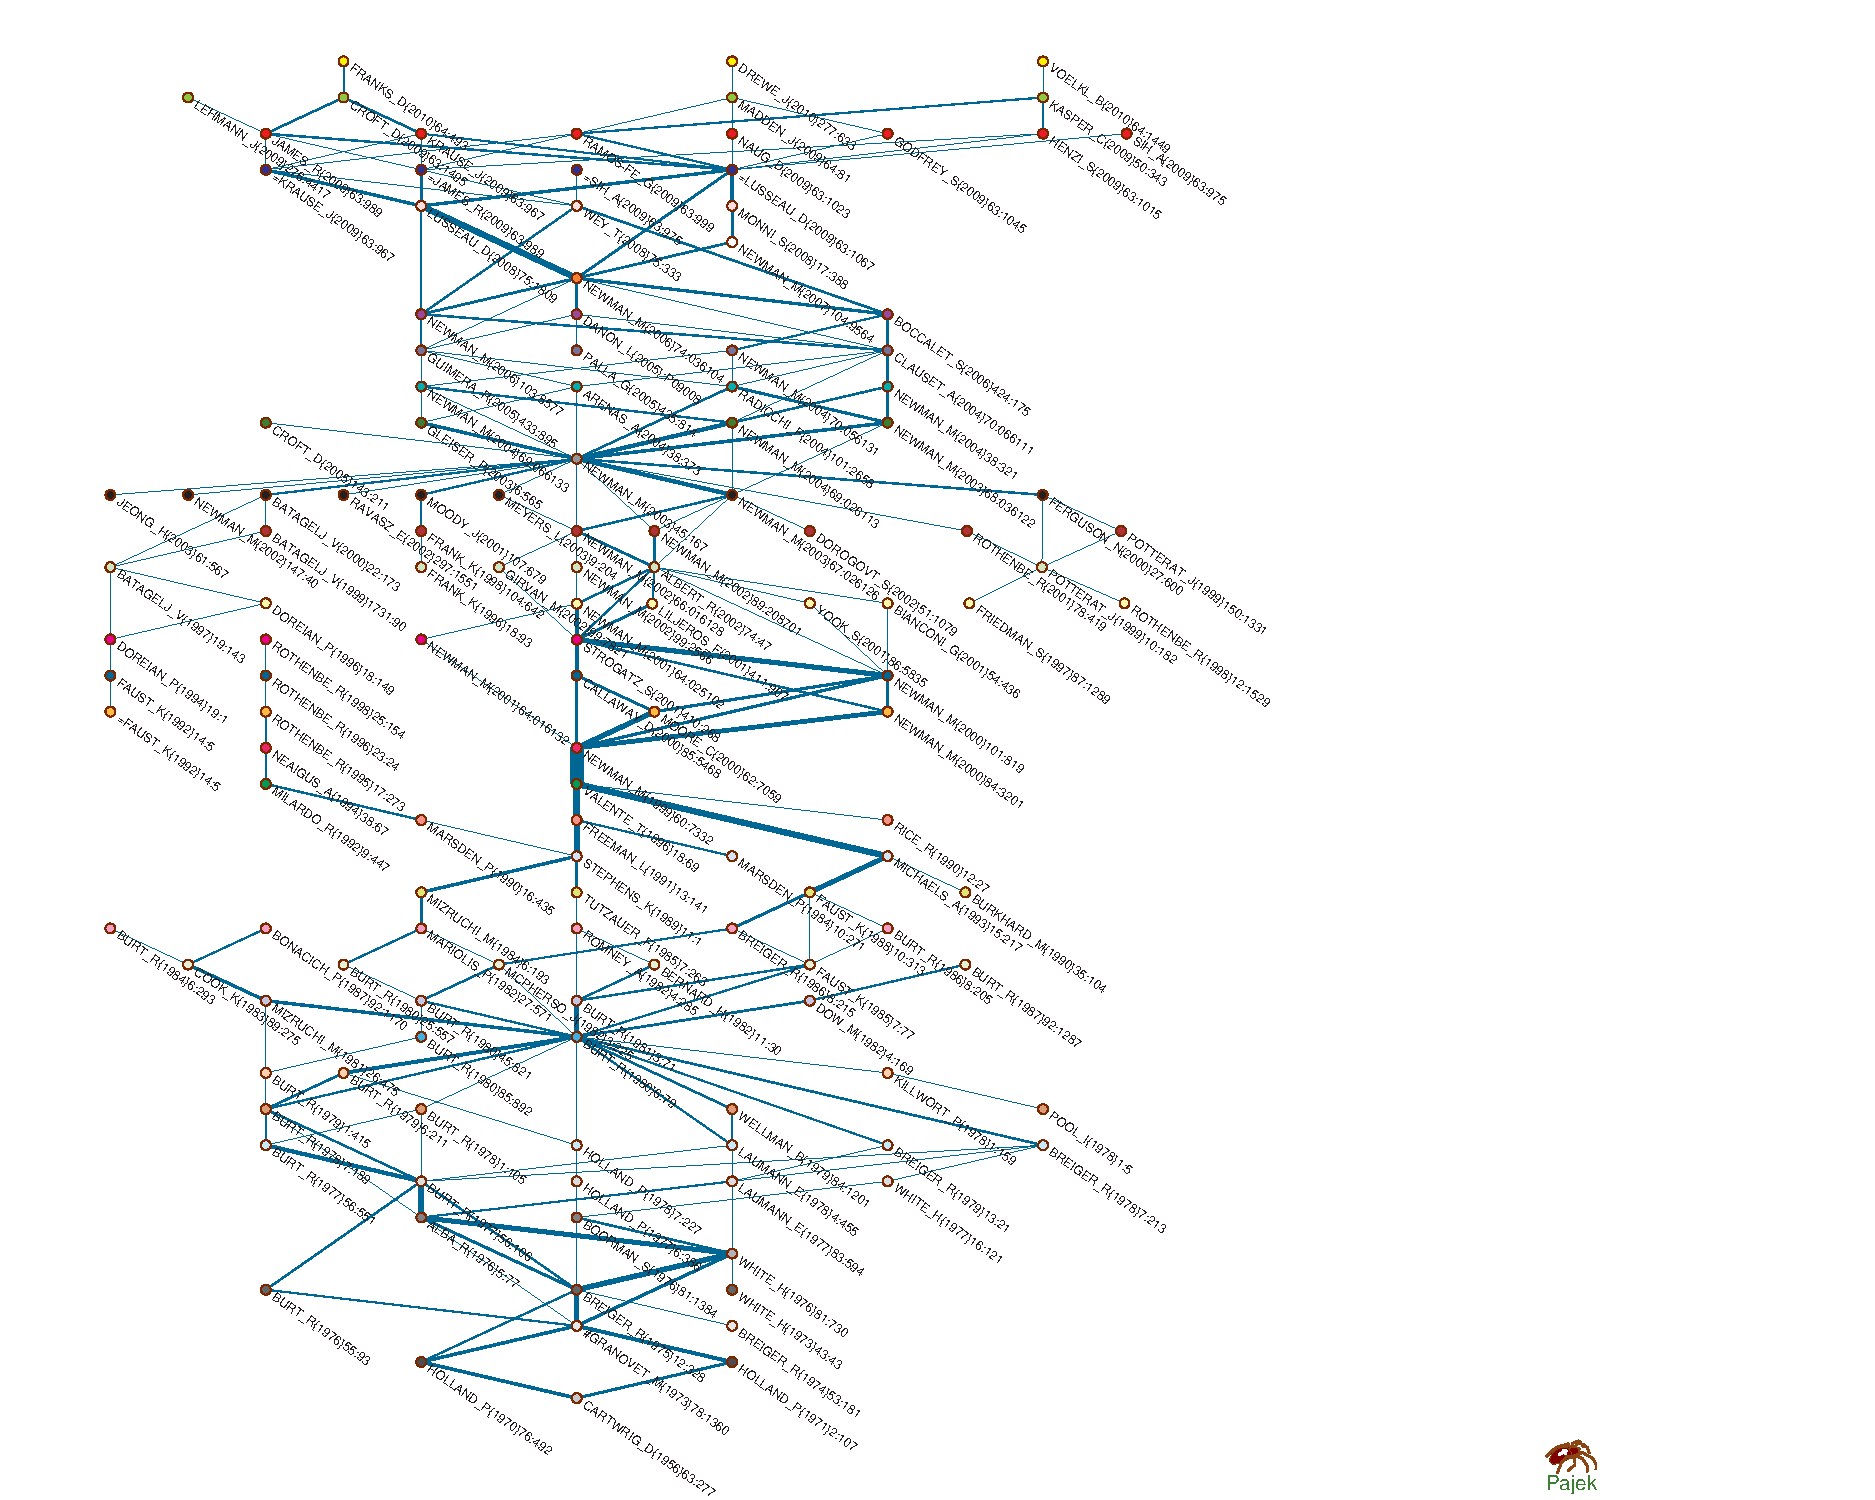
\includegraphics[width=\textwidth,viewport=45 0 615 695,clip=]{Island4Wxy.pdf}
\end{center}
\caption{Island 4, from SPC network} \label{island4}
\end{figure}

\begin{figure}
\begin{center}
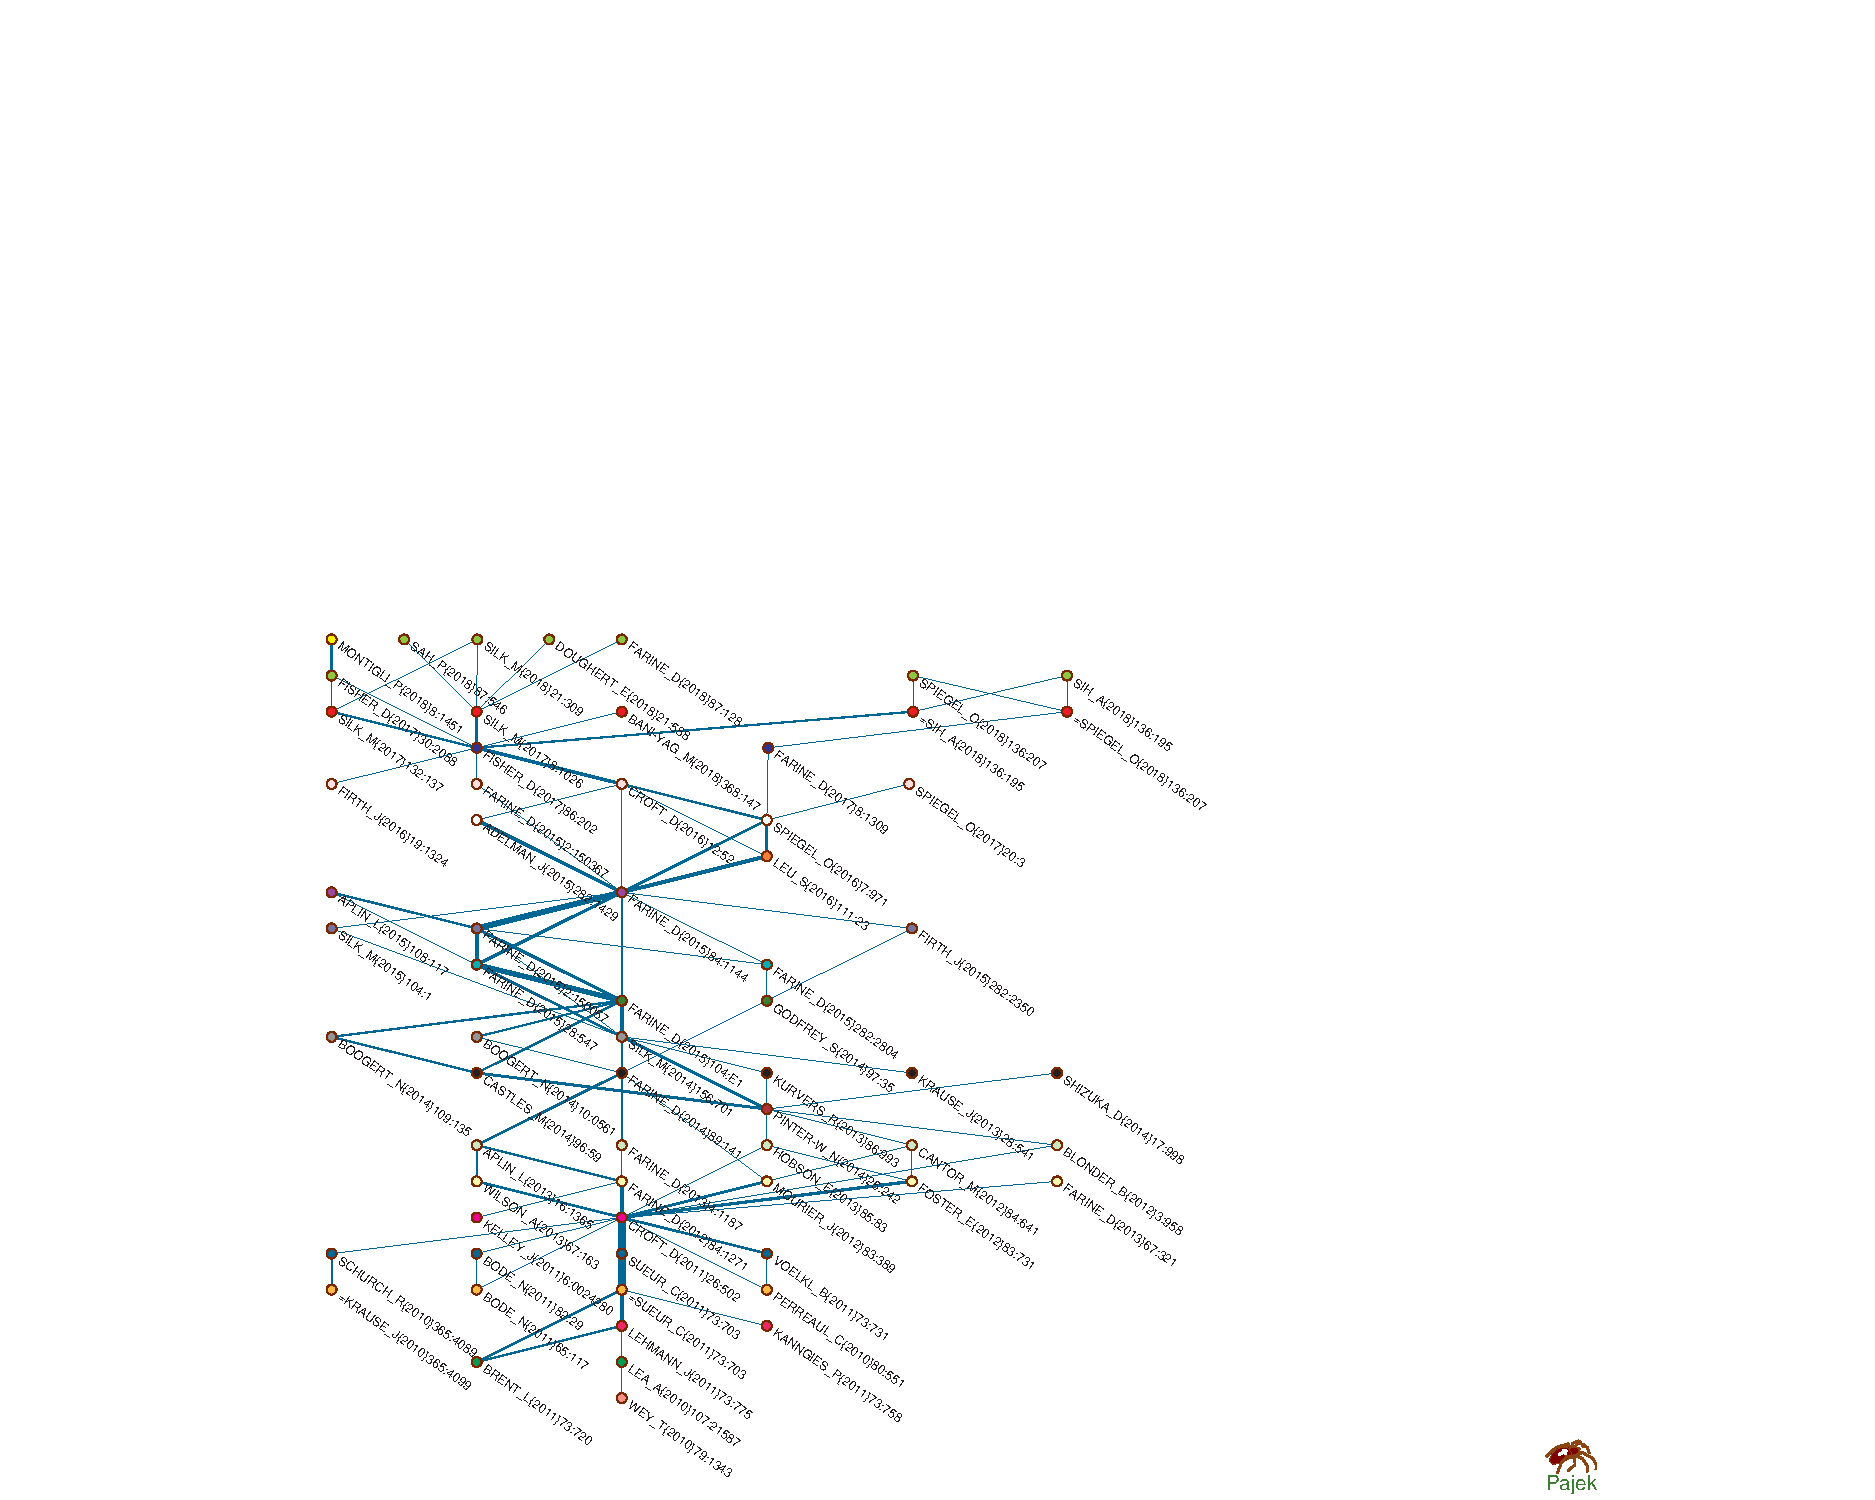
\includegraphics[width=\textwidth,viewport=150 5 585 420,clip=]{Island5Wxy.pdf}
\end{center}
\caption{Island 5, from SPC network} \label{island5}
\end{figure}

\begin{figure}
\begin{center}
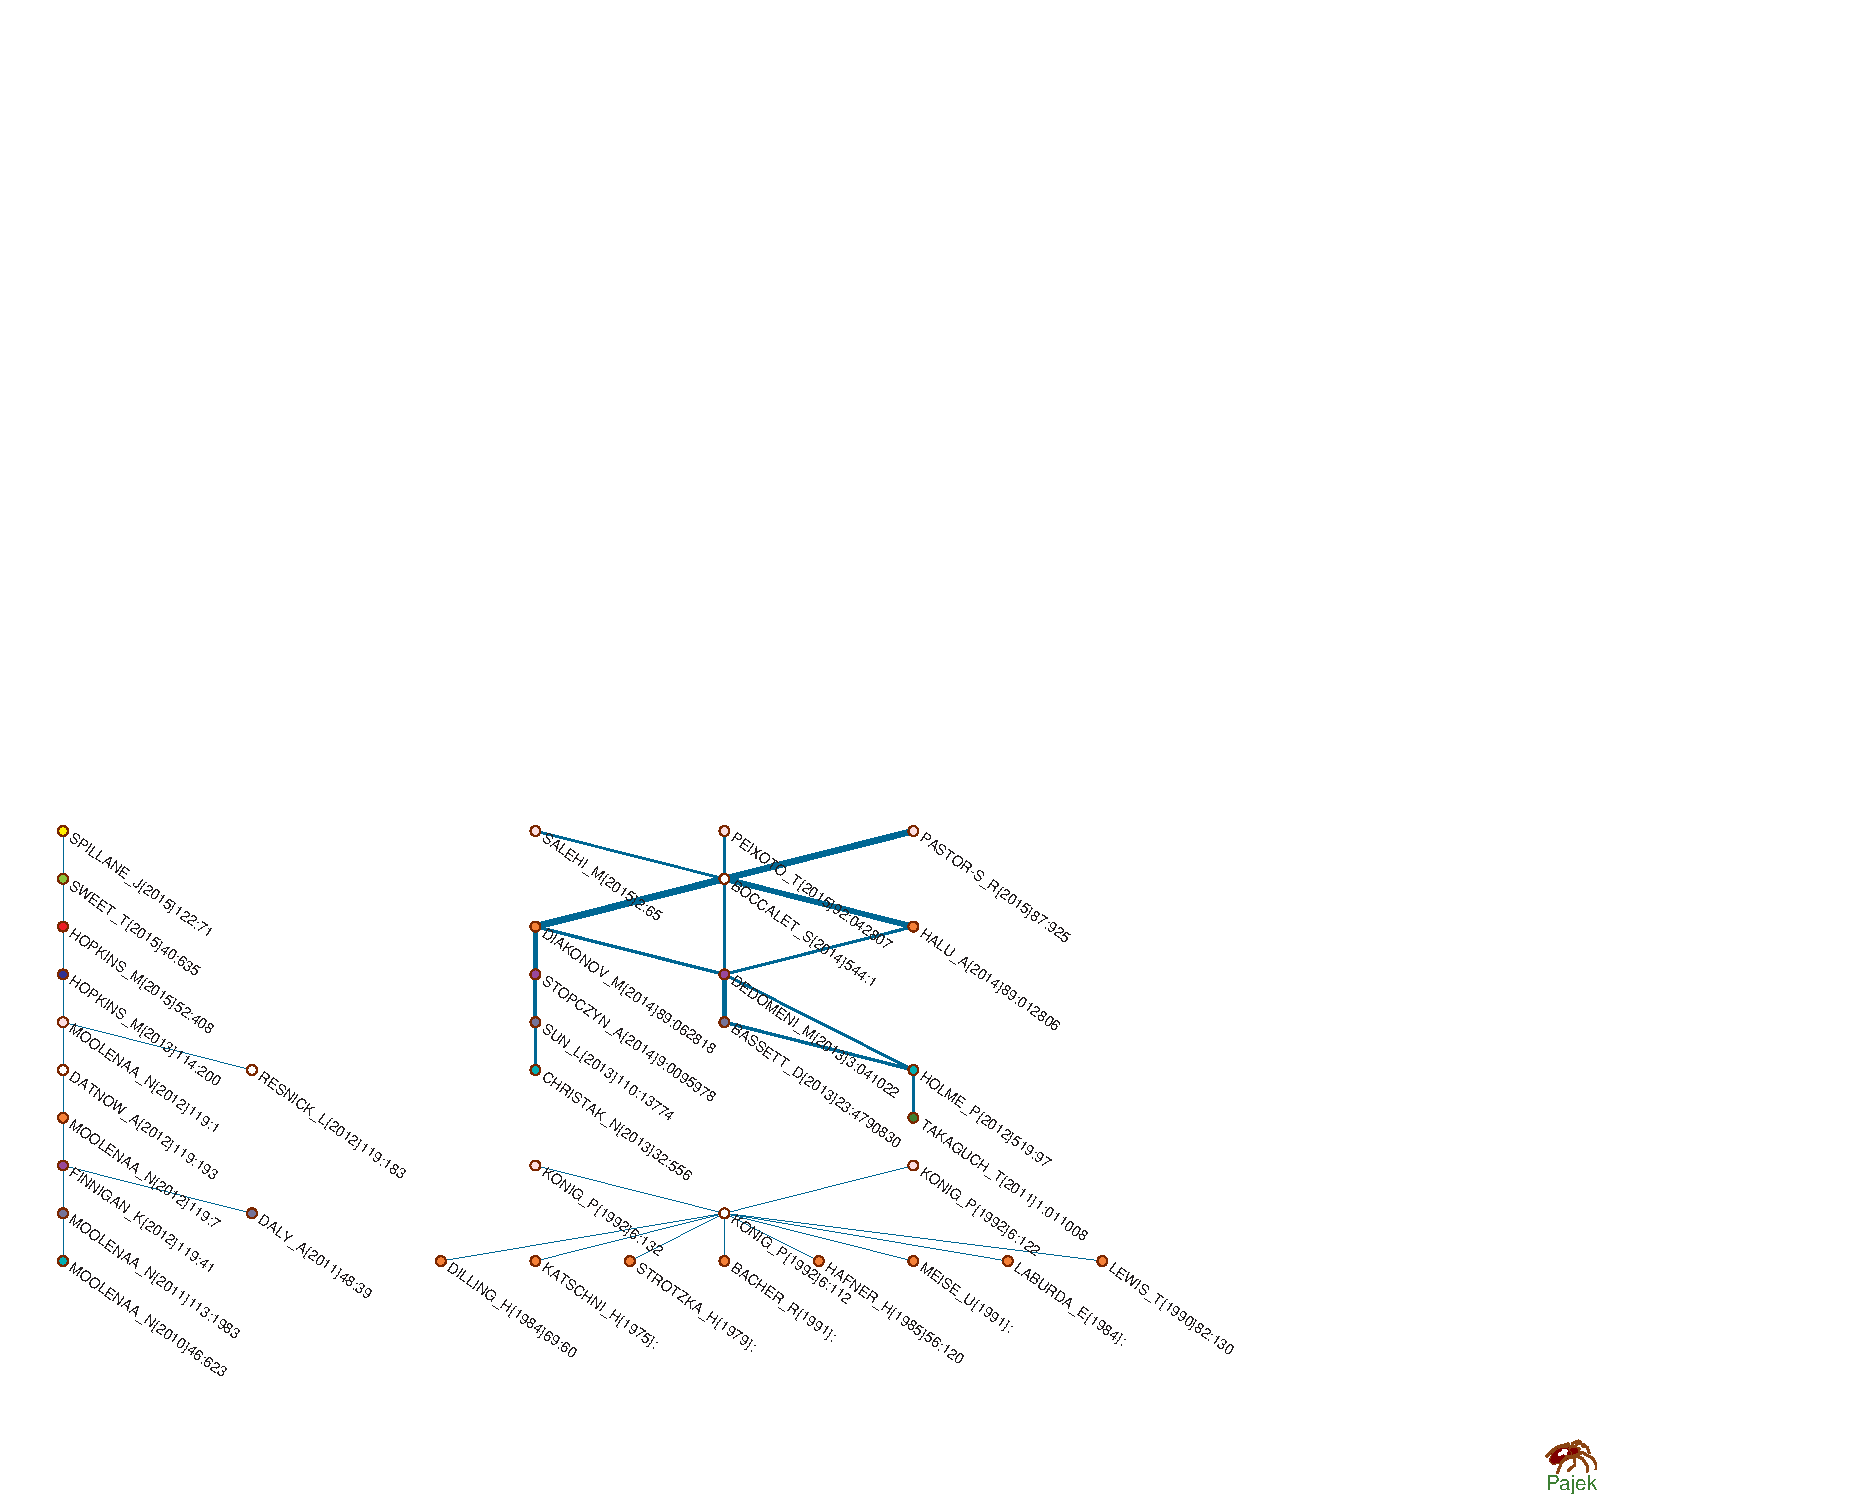
\includegraphics[width=\textwidth,viewport=25 55 595 330,clip=]{Island1-3Wxy.pdf}
\end{center}
\caption{Islands 1-3, from SPC network} \label{citeisl1-3}
\end{figure}

% Node Island (200) - will we present? 	
% SPC node islands [Vertex weights] of sizs  [20, 200] = 1 island of 200 nodes

%******************************************************************************

\subsection{Probabilistic flow}

We computed the Probabilistic flow on weighted network, and determined node islands (on vertex weights) with the number of nodes between 10 and 200 and got one island with the size of 200 nodes. \medskip    

Table~\ref{pFlow} present the list of the  most important works, which have the highest indegree values of Probabilistic flow network. For the purposes of visibility, the values were maximized by 1,000,000. 39 works from this list overlap with the table, obtained from the highest indegree values of network CiteN. First 30 works in the list, except \texttt{BLEI\_D(2003)3:993} on  latent dirichlet allocation, \texttt{ALBERT\_R(1999)401:130} on world-wide web, and \texttt{O`REILLY\_T(2005)} on web 2.0, are met in the both lists. Other works appeared in the top list of this island, which are not in the list of the most cited works, are works of physicists (Strogatz, Watts, Albert), computer scientists (Brin), mathematics (Bollobas), scientometrics (Page, Redner), and social scientists (Katz, Mitchell, Glaser). 

\begin{table}
\caption{Most important works from Probabilistic Flow network}\label{pFlow}\medskip
\small
\renewcommand{\arraystretch}{0.9}
\small
\begin{tabular}{c|c|l||c|c|l|l}
Rank&   	Value&   	Id&   	Rank&   	Value&   	Id\\ \hline
1&   	4691&   	WASSERMA\_S(1994):&   	31&   	545&   	BLONDEL\_V(2008):P10008\\
2&   	2941&   	WATTS\_D(1998)393:440&   	32&   	527&   	KATZ\_L(1953)18:39\\
3&   	2676&   	GRANOVET\_M(1973)78:1360&   	33&   	526&   	NEWMAN\_M(2010):\\
4&   	2445&   	BOYD\_D(2007)13:210&   	34&   	520&   	STROGATZ\_S(2001)410:268\\
5&   	2241&   	BARABASI\_A(1999)286:509&   	35&   	517&   	PALLA\_G(2005)435:814\\
6&   	1926&   	FREEMAN\_L(1979)1:215&   	36&   	499&   	CLAUSET\_A(2004)70:066111\\
7&   	1396&   	GIRVAN\_M(2002)99:7821&   	37&   	497&   	ERDOS\_P(1960)5:17\\
8&   	1299&   	NEWMAN\_M(2003)45:167&   	38&   	488&   	ROGERS\_E(2003):\\
9&   	1227&   	MCPHERSO\_M(2001)27:415&   	39&   	485&   	NEWMAN\_M(2006)103:8577\\
10&   	1158&   	ALBERT\_R(2002)74:47&   	40&   	481&   	COLEMAN\_J(1990):\\
11&   	1105&   	SCOTT\_J(2000):&   	41&   	478&   	BRIN\_S(1998)30:107\\
12&   	1098&   	BURT\_R(1992):&   	42&   	477&   	AMARAL\_L(2000)97:11149\\
13&   	1045&   	MILGRAM\_S(1967)1:61&   	43&   	475&   	ERDOS\_P(1959)6:290\\
14&   	1013&   	NEWMAN\_M(2004)69:026113&   	44&   	465&   	WATTS\_D(1999):\\
15&   	928&   	KAPLAN\_A(2010)53:59&   	45&   	462&   	LAVE\_J(1991):\\
16&   	878&   	FREEMAN\_L(1977)40:35&   	46&   	460&   	KLEINBER\_J(1999)46:604\\
17&   	852&   	PUTNAM\_R(2000):&   	47&   	449&   	SCOTT\_J(1991):\\
18&   	847&   	COLEMAN\_J(1988)94:95&   	48&   	446&   	BOLLOBAS\_B(1985):\\
19&   	835&   	BLEI\_D(2003)3:993&   	49&   	442&   	PAGE\_L(1999):\\
20&   	742&   	GRANOVET\_M(1985)91:481&   	50&   	440&   	NEWMAN\_M(2001)64:025102\\
21&   	731&   	CHRISTAK\_N(2007)357:370&   	51&   	436&   	NEWMAN\_M(2004)69:066133\\
22&   	727&   	EVERETT\_M(2002):&   	52&   	431&   	REDNER\_S(1998)4:131\\
23&   	726&   	NEWMAN\_M(2001)98:404&   	53&   	429&   	CHRISTAK\_N(2008)358:2249\\
24&   	719&   	ALBERT\_R(1999)401:130&   	54&   	424&   	ADOMAVIC\_G(2005)17:734\\
25&   	701&   	O'REILLY\_T(2005):&   	55&   	424&   	KEMP\_D(2003):137\\
26&   	669&   	BORGATTI\_S(2002):&   	56&   	423&   	DOMINGOS\_P(2001):57\\
27&   	667&   	FORTUNAT\_S(2010)486:75&   	57&   	423&   	MITCHELL\_J(1969):\\
28&   	633&   	HANNEMAN\_R(2005):&   	58&   	415&   	ALBERT\_R(2000)406:378\\
29&   	569&   	STEINFIE\_C(2007)12:1143&   	59&   	415&   	GLASER\_B(1967):\\
30&   	549&   	ZACHARY\_W(1977)33:452&   	60&   	410&   	ROGERS\_E(1995):\\ \hline
\end{tabular}
\end{table}

%******************************************************************************
\section{Authors Collaboration}  

In the following part, we present the patterns of collaboration between authors working in the field of Social netwirks analysis. This results are based on the analysis of the reduced network \textbf{WAr}. In general, there are different ways to create one-mode networks of collaboration between authors (AA) out of two-mode networks of works and authors (WA). These ways were presented and used in the previous works \citep{OnBibl,Understand}. Multiplying the original WAr network to transposed WAr network, and using different types of normalizations, we created three collaboration networks \textbf{Co}, \textbf{Cn}, and \textbf{Ct`}. The results are presented below. \medskip  

\subsection{Networks creation}  

The standard and the easiest way to obtain the collaboration network from the WA network was to make a \textbf{first collaboration network Co} \citep{OnBibl} by the multiplication of a transposed WA network (to AW) and initial one: \smallskip

\texttt{Co = t(WA) * WA = AW * WA = AA} \smallskip

In derived network  \textbf{Co}, the weight of the edges between the nodes is equal to total number of works author i and j wrote together. The degree of each author (node) is equal to the number of works he or she co-authored. The loops are equal to the total number of works that each author have (which is also equal to the indegree values of the WA network). \medskip 

It was proved, however, that the proposed approach has some limitations, such as the overrating of the contribution of works with many authors. That`s why the \textbf{fractional approach} \citep{OnBibl} was proposed which deals with the authors contribution in collaboration networks and propose different types of normalization. \medskip 

Thus, in the \textbf{second collaboration network Cn} the contribution of authors to their own works and works written with co-authors is considered. The normalization which is used create network n(WA) where the weight of each arc is divided by the sum of weights of all arcs having the same initial node as this arc (outdegree of a node) (for example, if the work has 3 authors, each weight is equal to 1/3). The network is constructed by the transposition of the WA network (to AW) and multiplying it with the (normalized) n(WA) network.\smallskip

\texttt{Cn = t(WA) * n(WA), where n(WA)[w,a] = WA[w,a] / outdeg(w)} \smallskip
 
In the derived network Cn, the weight of the edges between the nodes (authors) is equal to the contribution of author i to works, that he or she wrote together with author j (which can be not symmetric). The total contribution for a given work by all its authors is equal to the number of its authors. The total contribution for an author is equal to the number of works that he or she co-authored (indegree). The diagonal (loops) of the matrix is equal to the total contribution of author to his or her own works. Based on it, Batagelj and Cerinšek \citep{OnBibl} proposed \textbf{self-sufficiency index} as the proportion of author's contribution to his/her works and the total number of works he/she co-authored, and the \textbf{collaborativness index}, which is complementary to it (is equal to 1 minus self-sufficiency). \medskip 

Using another type of normalization - Newman normalization, who interpret the weight as a proportion of time spent for the collaboration with each co-author [Batagelj, slides], - the \textbf{fourth co-authorship network Ct`} \Remark{1st, 2nd, 4th - strange for reader?} was constructed, considering the total contribution of “strict collaboration” of authors i and j to works. In this case, for the initial WA network the weight of each arc is divided by the sum of weights of all arcs having the same initial node as this arc (outdegree of a node) subtracting the initial author (which is 1). Then the network Ct` is constructed by the transposition of the regularly normalized WA network (used for Cn network production) and multiplying it with this Newman normalized WA network. \smallskip

\texttt{Ct` = t(n(WA)) * n’(WA), where n’(WA)[w,a] = WA[w,a] / (outdeg(w)-1)} \smallskip

In the obtained network, the weights of the edges between the nodes (authors) are equal to the total contribution of “strict collaboration” of authors i and j to works they wrote together. The total contribution for an author is counted by line weights - it is equal to the sum of the weights of all the works he or she co-authored. \Remark{Description needs a check from Vlado} \medskip 

\subsection{Collaboration between authors}  

As it was already shown in the section 4.1. (Table~ \ref{numpap} the authors having the largest number of papers have (except Newman) Chinese names. In this sense, it is not productive to look at the `most writing' authors. However, from the \textbf{Co} network we still get an important information about collaboration between groups of authors. Figure~\ref{coPairs} shows the groups of authors, who have 20 and more works written together. Most of these authors are linked in pairs, however, some of these pair also produce cliques -- fully connected components.  \medskip  

\begin{figure}
\begin{center}
\includegraphics[width=0.7\textwidth,viewport=30 140 755 
660,clip=]{CoPairs.pdf}
\end{center}
\caption{Collaboration pairs} \label{coPairs}
\end{figure}

However, it is interesting to compare the values of the number of works that author has (in general, written by himself or herself or in collaboration) with the values of author`s contribution to these works and index of collaborativeness with others. Because of the `Chinese problem'  mentioned above we had to exclude the names of the Chinese authors from the output presented on the Table~\ref{collab}.  The names are ordered by authors` fractional total contribution to the field.\medskip  
 
The first rated author in sence of largest productivity is social scientist R. Burt, followed by phisician M. Newman. They are followed by P. Doreian, H. Park, and R. Dunbar. Other authors with large total contribution values are B. Wellamn, T. Valente, S. Park, P. Bonachich, L. Leidersdorf, C. Latkin, H. Litwin, and P. Marsden. There are a lot of authors representing social science in the table. The authors with the highest index of collaborativeness are marked in boldface. \medskip 

\begin{table}
\caption{Collaborativeness} \label{collab}\medskip
\small
\renewcommand{\arraystretch}{0.95}
\small
\begin{tabular}{c|l|p{1cm}|p{1cm}|p{1.5cm}||c|l|p{1cm}|p{1cm}|p{1.5cm}|} 
\# & Author & Total contribution & Total \# works & Collabora tiveness & \# & Author & Total contribution & Total \# works & Collabora tiveness \\ \hline
1& 	BURT\_R& 	55,73& 	71& 	0,22& 	31& 	\textbf{PATTISON\_P}& 	18,94& 	58& 	0,67\\
2& 	NEWMAN\_M& 	50,02& 	81& 	0,38& 	32& 	THELWALL\_M& 	18,41& 	37& 	0,5\\
3& 	DOREIAN\_P& 	46,19& 	72& 	0,36& 	33& 	KRACKHAR\_D& 	18,24& 	38& 	0,52\\
4& 	\textbf{PARK\_H}& 	41,94& 	113& 	0,63& 	34& 	FALOUTSO\_C& 	17,86& 	60& 	0,7\\
5& 	DUNBAR\_R& 	40,02& 	91& 	0,56& 	35& 	JACKSON\_M& 	17,78& 	38& 	0,53\\
6& 	WELLMAN\_B& 	36,43& 	63& 	0,42& 	36& 	\textbf{GONZALEZ\_M}& 	17,76& 	52& 	0,66\\
7& 	\textbf{VALENTE}\_T& 	34,96& 	97& 	0,64& 	37& 	MOODY\_J& 	17,7& 	40& 	0,56\\
8& 	\textbf{PARK\_S}& 	34,59& 	109& 	0,68& 	38& 	SCOTT\_J& 	17,54& 	28& 	0,37\\
9& 	BONACICH\_P& 	34& 	46& 	0,26& 	39& 	MORRIS\_M& 	17,22& 	43& 	0,6\\
10& 	LEYDESDO\_L& 	33,28& 	51& 	0,35& 	40& 	\textbf{RODRIGUE\_J}& 	15,9& 	52& 	0,69\\
11& 	LATKIN\_C& 	32,99& 	130& 	0,75& 	41& 	WASSERMA\_S& 	15,64& 	35& 	0,55\\
12& 	LITWIN\_H& 	32,42& 	50& 	0,35& 	42& 	KLEINBER\_J& 	15,05& 	34& 	0,56\\
13& 	MARSDEN\_P& 	30,17& 	39& 	0,23& 	43& 	BATAGELJ\_V& 	14,64& 	33& 	0,56\\
14& 	BORGATTI\_S& 	29,72& 	71& 	0,58& 	44& 	WILLIAMS\_A& 	14,5& 	31& 	0,53\\
15& 	SNIJDERS\_T& 	29,63& 	67& 	0,56& 	45& 	\textbf{SINGH\_A}& 	14,5& 	36& 	0,60\\
16& 	FRIEDKIN\_N& 	28,17& 	36& 	0,22& 	46& 	BRANDES\_U& 	14,39& 	35& 	0,59\\
17& 	CARLEY\_K& 	28,11& 	72& 	0,61& 	47& 	\textbf{BERKMAN\_L}& 	14,3& 	39& 	0,63\\
18& 	BARABASI\_A& 	27,61& 	67& 	0,59& 	48& 	MASUDA\_N& 	14,26& 	28& 	0,49\\
19& 	WHITE\_H& 	27,28& 	42& 	0,35& 	49& 	\textbf{SMITH\_A}& 	14,2& 	40& 	0,65\\
20& 	\textbf{CHRISTAK\_N}& 	22,89& 	74& 	0,69& 	50& 	LAZEGA\_E& 	14,17& 	26& 	0,46\\
21& 	EVERETT\_M& 	22,58& 	44& 	0,49& 	51& 	\textbf{CONTRACT\_N}& 	14,15& 	43& 	0,67\\
22& 	\textbf{KAZIENKO\_P}& 	21,97& 	64& 	0,66& 	52& 	\textbf{GONZALEZ\_A}& 	14,13& 	35& 	0,60\\
23& 	MARTINEZ\_M& 	21,9& 	53& 	0,59& 	53& 	\textbf{PENTLAND\_A}& 	14,12& 	41& 	0,66\\
24& 	\textbf{JOHNSON\_J}& 	21,19& 	54& 	0,61& 	54& 	FARINE\_D& 	14,04& 	34& 	0,59\\
25& 	\textbf{FOWLER\_J}& 	20,14& 	65& 	0,69& 	55& 	SCHNEIDE\_J& 	13,89& 	52& 	0,73\\
26& 	SKVORETZ\_J& 	20,07& 	42& 	0,52& 	56& 	WATTS\_D& 	13,67& 	27& 	0,49\\
27& 	FREEMAN\_L& 	20,03& 	27& 	0,26& 	57& 	FAUST\_K& 	13,5& 	25& 	0,46\\
28& 	BREIGER\_R& 	19,73& 	31& 	0,36& 	58& 	\textbf{SMITH\_M}& 	13,29& 	39& 	0,66\\
29& 	\textbf{ROBINS\_G}& 	19,67& 	64& 	0,69& 	59& 	\textbf{RODRIGUE\_M}& 	13,21& 	46& 	0,71\\
30& 	\textbf{RAHMAN\_M}& 	19,18& 	59& 	0,67& 	60& 	\textbf{RICE\_E}& 	13,09& 	48& 	0,73\\
\end{tabular}\\
\end{table}

Using Link islands approach, we extracted all the islands with the size between 5 and 50 nodes from the network \textbf{Ct`}. We got a large number of islands - 2,195 - with 14,227 nodes. Four largest island have, respectively, 35, 23, 21, and 19 nodes; other 70 islands have between 12 and 18 nodes. More then half of islands -- 58\% --  are composed of 5 nodes.  \medskip

The structures of the largest islands of size from 12 to 35 nodes is presented on the Figure (xx) (1,037 nodes). These subnetworks have different structures. Part of these structures are not very interesting: they are star-like networks, which represent one author collaborating with many others, or (almost) complete clusters (cliques), where all authors collaborate with (mostly) everyone else. However, some islands can be intesting to inspect - those large islands, which have more interesting structures \Remark{Create picture of Ct`\_Islands   (1-74), without labels, only structures }. \medskip

Another way to get interesting cases to inspect is to find the islands which have the strongest ties between the nodes. For this, we removed all the lines lower then certain trashold from the \textbf{Ct` net} and got the network of 32 nodes. Then we used and Simple islands approach and got simple line weight islands of size [2,50] out of the same network (number of islands = 14,222). Then we manualy searched for the islands to which these 32 nodes belong, and extracted them. We also found the islands for T. Snijders. These islands are presented below. Some of the authors having the strongest ties with each other goes from the field of social sciences (Everett and Boragatti, Pattison and Robins), some - from physics (Barabasi, Albert, Posfai), some - from both of the fields (Christakis and Fowler). \medskip

To better know what these authors are working at, we made an analysis of key words in coauthorship islands, which is presented in the following section \Remark{picture fromCt`\_largest line weights.net (100 nodes)}.  \medskip

%******************************************************************************

\section{Key words in coauthorship islands}

In this section we look at the key words for some of the islands inspected in the previous section. 

\subsection{Network creation}  

To construct the network of authors and keywords \textbf{AK}, we used normalized reduced networkds \textbf{WAr} and \textbf{WKr}.The first network was transposed and then multiplied with the second in the following way: \medskip

\texttt{nAWr x nWKr = AK}

\subsection{Key words in largest islands and islands with largest weights between the nodes}  

Using this two-mode network we can inspect all the keywords which are associated with each author. However, what is interesting is to look at the keywords for certain islands. Again, we start with the largest islands 1-3, which have, respectively, 35, 23, and 21 nodes. These islands are associated with large number of keywords, and on the Table~\ref{ak2} we present only those Top-15 keywords which were used more frequently. Besides the most common words (\textit{social, network}, and \textit{analysis}, there some specialized words that can characterize each island. For  Island 1 these are the keywords \textit{twitter, situation, emergence, crisis, uganda}, and others; for Island 2 - \textit{drug, risk, hiv, woman,infection}; for cluster Island 3 - \textit{radiation, radioactivity, environment, measurement}.  \medskip

Then we also looked at some certain islands with the largest values of weights between the nodes, which were identified before Table~\ref{akw}. We also had to present only Top-15 keywords for each cluster. For the group of authors with Barabasi in the center the keywords are \textit{web, dynamics, scale, complex, internet, world, free, random, evolve}. The island of Borgatti,  Everett, and Halgin is associated with the keywords \textit{graph, centrality, role, equivalence, semigroup, structure, clique, similarity}. The group of Fowler, Christakis, and Shakya have keywords \textit{spread, behavior, health, smoking, obesity, influence, evolution, dynamics}. Other group of social network analysts Robins and Pattison have the words \textit{model, graph, logit, logistic, regression, random, markov, exponential, p, semigroup, multirelational}. The group of Snijders have the keywords \textit{similarity, peer, model, network, family, orient, use, actor, social, behavior} which of course represent their work in stochastic actor-oriented models. \medskip

The large group of Litwin in the center connected to Stoekel and Shiovitz have the keywords \textit{health, support, older, life, people, adult, israel, elderly, old, age, american}. The group with large weight of lines between Grabowska and Kosinski have the keywords \textit{complex, model, dynamics, human, epidemic, spread, percolation, hierarchial}.The island of  Chinese authors wih strong ties between Wang and Ma have the keywords \textit{model, base, mobile, networking, online, trust, privacy}. \medskip

\begin{table}
\caption{Clusters of authors and keywords:\label{ak2} Largest islands 1,2,3 (2)}\medskip
\renewcommand{\arraystretch}{0.95}
\begin{center}
\begin{tabular}{p{1cm}|p{1cm}|p{2cm}|p{1cm}|p{2cm}|p{1cm}|p{2cm}}
& \multicolumn{2}{c}{Island1} & \multicolumn{2}{c}{Island2} & \multicolumn{2}{c}{Island3}\\ \hline
rank&	value&	keyword&	value&	keyword&	value&	keyword\\ \hline
1&	0.41&	social&	4.36&	social&	0.13&	radiation\\
2&	0.35&	network&	3.56&	network&	0.13&	public\\
3&	0.31&	twitter&	1.18&	use&	0.13&	open\\
4&	0.23&	situation&	0.91&	networking&	0.13&	measurement\\
5&	0.23&	emergency&	0.83&	structure&	0.13&	environment\\
6&	0.18&	narrative&	0.79&	drug&	0.13&	project\\
7&	0.18&	information&	0.78&	risk&	0.13&	collaborative\\
8&	0.17&	experience&	0.75&	hiv&	0.13&	radioactivity\\
9&	0.17&	crisis&	0.68&	user&	0.11&	community\\
10&	0.16&	uganda&	0.66&	woman&	0.11&	multimedia\\
11&	0.16&	approach&	0.62&	community&	0.11&	characteristic\\
12&	0.15&	categorization&	0.61&	sample&	0.11&	user\\
13&	0.15&	modeling&	0.59&	role&	0.11&	model\\
14&	0.15&	visualization&	0.56&	infection&	0.11&	share\\
15&	0.15&	ontology&	0.54&	new&	0.11&	distribution\\ \hline
Sum&	12.00&		& 89.76&		& 3.00&	\\ \hline
\end{tabular}
\end{center}
\end{table}

\begin{center}
\begin{table}
\caption{Clusters of authors and keywords:\label{akw} Clusters with largest line weights}\medskip
\begin{tabular}{p{0.7cm}|p{1cm}|p{2cm}||p{1cm}|p{2cm}||p{1cm}|p{2.1cm}||p{1cm}|p{1.7cm}}
 &	clu &	repr &	clu &	repr &	clu &	repr &	clu &	repr \\ \hline
&	13381&	Barabasi&	13418&	Grabowska&	14112&	Wang&	6439&	Litwin\\\hline
rank&	value&	keyword&	value&	keyword&	value&	keyword&	value&	keyword\\ \hline
1&	8.31&	network&	2.12&	network&	17.54&	social&	4.32&	social\\
2&	2.29&	social&	1.98&	social&	17.21&	network&	4.11&	network\\
3&	2.08&	web&	1.58&	complex&	4.85&	model&	2.64&	health\\
4&	2.04&	dynamics&	1.23&	model&	4.80&	base&	2.54&	support\\
5&	2.04&	scale&	1.10&	dynamics&	3.56&	mobile&	2.25&	older\\
6&	1.87&	complex&	0.99&	human&	3.47&	analysis&	1.86&	life\\
7&	1.87&	internet&	0.90&	epidemic&	2.49&	information&	1.66&	people\\
8&	1.78&	world&	0.64&	spread&	2.45&	community&	1.63&	adult\\
9&	1.64&	community&	0.60&	percolation&	2.07&	networking&	1.45&	type\\
10&	1.49&	free&	0.43&	line&	2.04&	online&	1.31&	israel\\
11&	1.41&	model&	0.39&	society&	1.96&	trust&	1.21&	elderly\\
12&	1.31&	science&	0.36&	hierarchical&	1.81&	algorithm&	1.01&	old\\
13&	1.20&	link&	0.35&	pattern&	1.67&	privacy&	1.00&	age\\
14&	1.20&	random&	0.28&	opinion&	1.59&	complex&	0.82&	american\\
15&	1.20&	evolve&	0.28&	formation&	1.54&	behavior&	0.81&	later\\ \hline
Sum&	89.55&	&	21.67&	&	267.40&	&	76.14&	\\ \hline\hline
 &	clu &	repr &	clu &	repr &	clu &	repr &	clu &	repr \\ \hline
&	13946&	Borgatti&	14024&	Christakis&	14221&	Robins&	13916&	Snijders\\ \hline
rank&	value&	keyword&	value&	keyword&	value&	keyword&	value&	keyword\\ \hline
1&	7.60&	network&	3.72&	network&	2.80&	network&	3.93&	network\\
2&	3.94&	social&	3.46&	social&	2.48&	social&	3.04&	social\\
3&	3.29&	graph&	1.16&	spread&	2.30&	model&	2.48&	model\\
4&	2.13&	centrality&	1.15&	behavior&	1.57&	graph&	1.78&	graph\\
5&	2.09&	analysis&	0.88&	health&	1.15&	logit&	1.35&	dynamics\\
6&	2.02&	regular&	0.67&	large&	1.15&	analysis&	1.22&	markov\\
7&	2.02&	role&	0.63&	smoking&	1.12&	logistic&	1.11&	random\\
8&	1.96&	equivalence&	0.60&	model&	1.12&	regression&	0.97&	statistical\\
9&	1.73&	semigroup&	0.54&	human&	1.02&	random&	0.95&	datum\\
10&	1.48&	structure&	0.50&	obesity&	1.01&	markov&	0.84&	friendship\\
11&	1.21&	relation&	0.50&	life&	0.94&	exponential&	0.84&	inference\\
12&	1.20&	clique&	0.49&	cooperation&	0.84&	p&	0.76&	behavior\\
13&	1.13&	similarity&	0.48&	influence&	0.77&	statistical&	0.75&	influence\\
14&	1.12&	ebloc&	0.46&	evolution&	0.70&	semigroup&	0.73&	analysis\\
15&	1.00&	correction&	0.45&	dynamics&	0.67&	multirelational&	0.70&	peer\\ \hline
Sum&	92.66&	&	55.75&	&	47.89&	&	66.62&	\\
\end{tabular}
\end{table}
\end{center}


%******************************************************************************
\section{Citation among authors}

After analysing Cite network and WA network and looking at citations between works and collaborations between authors separately, we can also look at the derieved \textbf{CiteA network}, which shows citations among authors. \medskip 

\subsection{Network creation} 

To get information about citations among authors we computed the \textbf{derived CiteA} networkas a product of multiplication of the networks \textbf{WAr} and \textbf{CiteR}.cIn this network, the value of element CiteA[u;v] is equal to the number of citations from works coauthored by u to works coauthored by v. \smallskip

\texttt{CiteA=t(WAr) * CiteR * WAr} \smallskip

We also produced the normalized version of this network, \textbf{CiteAn}, where the value of element CiteAn[u;v] is equal to the number of {fractional} contribution of citations from works coauthored by u to works coauthored by v.\smallskip

\texttt{CiteA=t(WAr) * nCiteR * WAr} \smallskip

\subsection{Citations} 

After the exploratory analysis of the obtined networks, we had to exclude the top-cited work of Wasserman and Faust (\texttt{[WASSERMA\_S(1994):}] from the data set as a lot of nodes were connected to it. \medskip

Then we used Islands approach to get islands of the size [5, 200] from the \textbf{CiteA}. However, the combination of nodes with large number of citations (to Wasserman, Granovetter, Boyd, Newman) with the `Chinese cloud', which was already identified above, blured the results. This why the normalized network \textbf{CiteAn} was used for identification of islands. We got 195 islands of size between 5 and 200. \medskip 

The Main island of \textbf{CiteAn} network consits of 200 nodes. In this network, citations separates between M. Granovetter and D. Boyd, each of them have their own `cloud' of other authors. They are also connected through several authors citing both of them. However, most of these authors are againg from the `Chinese group' \Remark{Picture CiteAn\_Island1(200)}.  \medskip  

%pictures CiteAn_Main Island - has 212 nodes. I looked at the network, and extracted Island1 again - it is file CiteAn_Island1(200). They are different. Probably, first one - is the main island frim CiteA not normalized?

Figure XX presents other 21 islands consisted of minimum 10 nodes (in sum, 268 nodes). Most of these islands are star-like, meaning that the author in the center actively cites a set of other authors. There are also two more `clique-like' islands, identifying groups of connected authors who cites each other. However, there are several more interesting structures (1, 2, 3), which shows several groups of authors connected to each other \Remark{picture CiteAn\_Islands2-22}. \medskip  

\section{Co-citation among authors. Bibliographic Coupling }

\subsection{Network creation} 

Jaccard - ? \Remark{Try to compute}

%******************************************************************************
\section{Citation among journals}

In this section, we present the results on the citations between journals featuring works in the area of Social network analysis. 

\subsection{Network JJf creation}

To get information about citations among journals we computed the \textbf{derived JJf} network, which takes into account citations from papers published in journal \textit{i} to papers published in journal \textit{j}, which appeared in the works included into the \textbf{WJr net}. We used a \textbf{CiteR net} to get information on citations between works. As journals of different sizes were included into the data set, using the \textit{fractional approach} this network was normalized. Then the networks were multyplied in the following way. Thus, the weights in the obtained network take into account \textit{fractional} contribution of citations from papers published in journal \textit{i} to papers published in journal \textit{j}.   \medskip 

\texttt{JJf = t(WJr) * n(CiteR) * WJr}

\subsection{Citations}

Looking at the loops of the network \textbf{JJr}, we got the list of journals with highest self-citation (Table~\ref{jselfcite}). The highest value belongs to the \textit{Social Networks} journal, which is one of the main journals in the field of Social network analysis. Second highest ranked journal is the \textit{Computers in Human Behavior} -- the one in the field of Computer interactions and Cyberpsychology. Other quite highly ranked journals are \textit{Physica A-Statistical Mechanics And Its Applications, Journal of Computer-Mediated Communication, Social Science \& Medicine, and American Journal of Sociology}. However, we note that the differences between values of first and last mentioned journals are quite significant. \medskip 

\begin{table}
\caption{Journals with the highest self-citation} \label{jselfcite}\medskip
\renewcommand{\arraystretch}{0.95}
\small
\begin{center}
\begin{tabular}{c|l|l} 
\# &	Value&	Journal  \\  \hline 
1&	1083,68&	SOC NETWORKS\\
2&	533,84&	COMPUT HUM BEHAV \\
3&	212,1&	LECT NOTES COMPUT SC \\
4&	163,32&	PHYSICA A\\
5&	135,71&	J COMPUT-MEDIAT COMM\\
6&	111,53&	SOC SCI MED\\
7&	110,49&	AM J SOCIOL\\
8&	84,33&	SCIENTOMETRICS\\
9&	68,29&	CYBERPSYCH BEH SOC \\
10&	55,33&	NEW MEDIA SOCI\\
11&	54,94&	J MED INTERNET RES\\
12&	54,48&	EXPERT SYST APPL\\
13&	51,01&	ANIM BEHAV\\ \hline 
\end{tabular} \\ 
\end{center}
\end{table}  

We also generated Islands of size between 2 and 5, and got 115 islands, with the largest island containing 50 nodes. The Main islands is presented on the Figure~\ref{jjFmain}. There are three groups of journals: two large groups of journals in Social Sciences and Computer Science, as well as one smaller group of journals in Physics. Citations among journals have clear acyclic (hierarchical) organization. \medskip 

In the Social Sciences group, the most citing journal is \textit{Social Networks}, which is strongly connected to the \textit{Amercian Journal of Sociology}, as well as have connections with many other sociological journals (\textit{Structural Analysis in Social Sciences, American Sociological Review, Social Forces, Journal of Mathematical Sociology, Social Network Analysis}, which are, in turn, also have connections to the American Journal of Sociology. This journal is also cited by a large number of other journals from differnt fields of Social sciences: Sociology, Family studies, Social work, Psychology, Behavioral science, Communication, Migration studies, Business, Management, Organization studies, Urban and Rural studies. \medskip 

In the Computer Science group of journals, the most citing position is taken by \textit{Computers in Human Behavior} journal, which is largerly citing \textit{Journal of Computer-Mediated Communication}, as well as \textit{CyberPsychology \& Behavior, Cyberpsychology, Behavior, and Social Networking}, which are are also connected to it, and the \textit{American Journal of Sociology}. \textit{Journal of Computer-Mediated Communication} is also cited by other journals from Somputer sciences, Education technology. \medskip 

Two top cited journals have shared journals which cite both of them. They are \textit{Information, Communication \& Society, Communications in Computer and Information Science, Lecture Notes in Artificial Intelligence, New Media \& Society}. The journal with the largest citations of both of these jornals is \textit{Lecture Notes in Computer Science}, which is also citing other journals, such as \textit{Social Networks, Structural Analysis in Social Science}, and \textit{Nature}.\medskip 

The Physics group is presented by the journals \textit{Physica A-Statistical Mechanics And Its Applications, Physical Review E}, and also include some interdisciplinary journals \textit{Plos One}, \textit{Science}, and \textit{Nature}. There are links from \textit{Physica A} and \textit{Plos One} to  the \textit{American Journal of Sociology}. \medskip  

Other islands (2-11) of journals citing each other (including minimum 3 journals) are the ones on the topics of substance abuse and addiction; archeology, anthropology and antiquity, behavioral ecology and animal behavior; geriatric psychiatry; psychology and deviation; child psychology and psychiatry; medicine; family medicine, sexual and reproductive health; speech-language; computer graphics. \medskip  

\begin{figure}
\begin{center}
\includegraphics[width=0.9\textwidth,viewport=35 0 965 
740,clip=]{JJfMain.pdf}
\end{center}
\caption{Citations among journals -- main island} \label{jjFmain}
\end{figure}

Other islands 12-115 contain only 2 nodes - they are pairs of journals. Journals with the largest weights of lines are presented on the Table~\ref{jpairs}. The links are directed: first written journal cites second one. These journals cover the wide range of disciplines, including Health studies, Epidemiology, Medicine, Surgery, Veterinary, Biotechnology, Psychiatry, Family studies, Neuroscience, Education, Sport, Archeology, Ethnology, Anthropology, History, Engineering, Mobile computing, Information science.  

\begin{table}
\caption{Pairs of journals} \label{jpairs}\medskip
\renewcommand{\arraystretch}{0.9}
\small
\begin{tabular}{c|l|p{6cm}||c|l|p{6cm}|}
\# &	Value&	Journals &	\# &	Value&	Journals \\  \hline 
1&	17,38&	SEX TRANSM DIS --  AIDS       &	21&	4&	IEEE INT SYMP INFO --  IEEE T INFORM THEORY   \\
2&	14,17&	PREV VET MED --  TRANSBOUND EMERG DIS     &	22&	4&	HEALTH RISK SOC --  RISK ANAL      \\
3&	10,47&	ACTA PSYCHIAT SCAND --  BRIT J PSYCHIAT     &	23&	4&	QUAL RES SPORT EXERC --  SPORT MANAG REV    \\
4&	10,27&	IEEE T PARALL DISTR --  IEEE INFOCOM SER    &	24&	4&	UROL ONCOL-SEMIN ORI --  BJU INT      \\
5&	8,1&	IEEE T VEH TECHNOL --  IEEE T MOBILE COMPUT   &	25&	4&	PSYCHIAT DANUB --  QJM-INT J MED      \\
6&	6,77&	J CONSTR ENG M --  J CONSTR ENG M ASCE  &	26&	4&	COMMUNITY DENT ORAL --  J AM DENT ASSOC    \\
7&	5,68&	SOC COGN AFFECT NEUR --  NEUROIMAGE      &	27&	4&	Z ETHNOL --  J SOC HIST      \\
8&	5&	APHASIOLOGY --  ADULT EDUC QUART       &	28&	4&	J AM SOC HYPERTENS --  NAT BIOTECHNOL     \\
9&	4,67&	J INTELL DISABIL RES --  J APPL RES INTELLECT   &	29&	4&	MATERN CHILD HLTH J --  J NERV MENT DIS   \\
10&	4,67&	APPL ENERG --  ENERG BUILDINGS       &	30&	4&	TRANSPL P --  AM J TRANSPLANT      \\
11&	4,67&	J ISL COAST ARCHAEOL --  ANTIQUITY      &	31&	4&	J AFFECT DISORDERS --  DEATH STUD      \\
12&	4,67&	INFORM SOC-ESTUD --  PERSPECT CIENC INF      &	32&	4&	J NEW APPROACHES EDU --  ESTUD SOBRE MENSAJ P   \\
13&	4,5&	J ACAD LIBR --  REF USER SERV Q    &	33&	4&	J ADDICT NURS --  CLIN PSYCHOL REV     \\
14&	4,18&	CIENC SAUDE COLETIVA --  CAD SAUDE PUBLICA     &	34&	4&	INT J CARDIOL --  WIRES DATA MIN KNOWL    \\
15&	4&	ETHN DIS --  HEART LUNG       &	35&	4&	MCN-AM J MATERN-CHIL --  AM J NURS     \\
16&	4&	EPIDEMIOL PREV --  HUM VACC IMMUNOTHER      &	36&	4&	INT J PEDIATR-MASSHA --  BEHAV MED      \\
17&	4&	OPTIM LETT --  ARTIF LIFE       &	37&	4&	HEALTH EXPECT --  CAN J CARDIOL      \\
18&	4&	ACTAS UROL ESP --  AESTHET SURG J     &	38&	4&	ARCTIC ANTHROPOL --  ARCTIC        \\
19&	4&	J RETAIL CONSUM SERV --  AUSTRALAS MARK J    &	39&	4&	REV BRAS ENFERM --  REV LAT-AM ENFERM     \\
20&	4&	J MARITAL FAM THER --  J CONSTR PSYCHOL    &	40&	3,36&	J CHILD PSYCHOL PSYC --  J AUTISM DEV DISORD   \\ \hline 
\end{tabular}\\
\end{table}  


%******************************************************************************
\section{Conclusions}

%Basic statistics of derived networks allow us to get the most important works, authors, journals, keywords. \medskip

%Citation network analysis reveals its main structure - gropus of works which are connected with each other. Obtained components are interlinked. \medskip

%Deeper analysis of other derived networks, including those which can be constructed out of different initial ones (e.g., WA and WK), will show other patterns of Social Network Analysis field development. 

%******************************************************************************

\begin{thebibliography}{99}
\bibitem[Batagelj et al.(2014)]{Understand}
Batagelj, V., Doreian P., V., Ferligoj, A., Kejžar N. (2014). Understanding Large Temporal Networks and Spatial Networks: Exploration, Pattern Searching, Visualization and Network Evolution. 
\bibitem[Freeman(2004)]{SNAdev}
   Freeman, L. (2004). The development of social network analysis. A Study in the Sociology of Science, 1.
\bibitem[Hummon and Carley(1993)]{normSci}
   Hummon, N. P., Carley, K. (1993). Social networks as normal science. Social networks, 15(1), 71-106.
\bibitem[Otte and Rousseau(2002)]{SNAinf}
   Otte, E., Rousseau, R. (2002). Social network analysis: a powerful strategy, also for the information sciences. Journal of information Science, 28(6), 441-453. 
\bibitem[Barabasi et al.(2002)]{Evol}
    Barabâsi, A. L., Jeong, H., Néda, Z., Ravasz, E., Schubert, A., Vicsek, T. (2002). Evolution of the social network of scientific collaborations. Physica A: Statistical mechanics and its applications, 311(3-4), 590-614.
\bibitem[Batagelj and Cerinšek(2013)]{OnBibl}    
   Batagelj V., Cerinšek M.(2013). On bibliographic networks. Scientometrics. 96 (3), 845-864
\bibitem[Batagelj et al.(2017)]{PeerRew}    
   Batagelj, V., Ferligoj, A. Squazzoni, F. The emergence of a field: a network analysis of research on peer review. Scientometrics (2017) 113: 503. https://doi.org/10.1007/s11192-017-2522-8  
\bibitem[Moody(2004)]{moody}     
   Moody, J. (2004). The structure of a social science collaboration network. American Sociological Review, 69, 213–238
\bibitem[Hunter and Leahey(2008)]{sociol}     
   Hunter, L., Leahey E. (2008). Collaborative Research in Sociology: Trends and Contributing Factors. American Sociologists, 39, 4, 290-306. 
\bibitem[Pontille(2003)]{pontille}     
   Pontille, D. (2003). Authorship Parctices and Institutional Contexts in Sociology: Elements for a Comparison of the United States and France, Science, Technology and Human Values, 28, 2, 217-234.
   \bibitem[Mali et al.(2010)]{mali}     
   Mali, F., KroneggerL., Ferligoj, A. (2010). Co-authorship trends and collaboration patterns in the Slovenian sociological community. Corvinus journal of sociology and social policy, 1(2), 29-50.
   \bibitem[Sokolov et al.(2012)]{sokolov}     
   Sokolov M.M., Safronova, M.A., Guba, K.S., Dimke, D.V. Intellectual landscape and social structure of the local academic community (the case of St. Petersburg sociology) // Preprint.Humanities research. WP6. Higher School of Economics, 2012. No. WP6 / 2012/01.
 \bibitem[Hou et al.(2008)]{hou}     
   Hou, H., Kretschmer, H., Liu, Z. (2008). The Structure of Scientific Collaboration Networks in Scientometrics. Scientometrics, 75,189. 10.1007/s11192-007-1771-3 
 \bibitem[Chinchilla-Rodríguez et al.(2012)]{rodriguez}   
   Chinchilla-Rodríguez, Z., Ferligoj, A., Miguel, S., Kronegger, L., Moya-Anegon, F. (2012). Blockmodeling of co-authorship networks in library and information science in Argentina: A case study. Scientometrics. 93. 699-717. 10.1007/s11192-012-0794-6.
 \bibitem[Lopaciuk-Gonczaryk(2016)]{polish}   
   Lopaciuk-Gonczaryk, B. (2016). Collaboration strategies for publishing articles in international journals – A study of Polish scientists in economics. Social Networks, 44, 50-63.
    \bibitem[Carley et al.(1993)]{conflict}   
   Carley, K. M., Hummon, N. P., Harty, M. (1993). Scientific influence: An analysis of the main path structure in the Journal of Conflict Resolution. Knowledge, 14(4), 417-447.
    \bibitem[Hummon and Doreian(1989)]{dna}   
   Hummon N.P., Doreian P.(1989). Connectivity in a citation network: The development of DNA theory. Social Networks, 11, 1, 39-63. 
    \bibitem[Newman(2004)]{newman4}     
   Newman, M.E.J. (2004). Coauthorship networks and patterns of scientific collaboration. Proceedings of the National Academy of Sciences of the United States of America 101(Suppl1), 5200–5205. 
    \bibitem[Newman(2001)]{newman1}     
   Newman, M.E.J. (2001). Scientific collaboration networks. II. Shortest paths, weighted networks, and centrality. Physical Review E, 64. 
    \bibitem[Cugmas et al.(2016)]{cugmas}        
   Cugmas M., Ferligoj A., Kronegger L. (2016). The stability of coauthorship structures. Scientometrics. 106(1), 163–186.10.1007/s1119201517904
    \bibitem[Ferligoj et al.(2015)]{ferligoj}        
   Ferligoj A., Kronegger L., Mali F., Snijders T., Doreian P. Scientific collaboration dynamics in a national scientific system. Scientometrics.
    \bibitem[Kronegger et al.(2012)]{kroneg}      
   Kronegger L., Mali F., Ferligoj A., Doreian P. (2012). Collaboration structures in Slovenian scientific communities. Scientometrics, 90, 631-647. 10.1007/s11192-011-0493-8. 
    \bibitem[Kronegger et al.(2004)]{glaenzel}      
   Glaenzel, W., Andreas, S. (2004). Analysing scientific networks through co-authorship, in: Henk F., Moed et al., ed., Handbook of Quantitative Science and Technology Research. The Use of Publication and Patent Statistics in Studies of S\&T Systems, Dordrecht, Boston, London, Kluwer Academic Publishers, 257-276.
    \bibitem[Wagner and  Leydesdorff(2005)]{wagner}      
   Wagner, C. S.,  Leydesdorff, L. (2005). Network structure, self-organization, and the growth of international collaboration in science. Research policy, 34(10), 1608-1618.
    \bibitem[Leydesdorff et al.(2008)]{leydes}      
   Leydesdorff L., Schank T., Scharnhorst A., De Nooy W. (2008). Animating the development of Social Networks over time using a dynamic extension of multidimensional scaling / El Profesional de Informacion, 17(6).
    \bibitem[Hummon et al.(1990)]{central}   
   Hummon N.P., Doreian P., Freeman L.C. (1990). Analyzing the Structure of the Centrality-Productivity Literature Created Between 1948 and 1979 / Science Communication. 11, 4, 459 – 480. 
    \bibitem[Kejžar et al.(2010)]{kejzar}   
Kejžar, N., Černe, S. K., Batagelj, V. (2010). Network analysis of works on clustering and classification from web of science. In Classification as a Tool for Research, 525-536. Springer, Berlin, Heidelberg.
    \bibitem[Brandes, Pich(2011)]{brandes}  
Brandes, U., Pich, C. (2011). Explorative visualization of citation patterns in social network research. Journal of social structure, 12(8), 1-19.
    \bibitem[Lazer et al.(2009)]{lazer}  
Lazer, D., Mergel, I., and Friedman, A. (2009). Co-citation of prominent social network articles in sociology journals: The evolving canon. Connections, 29(1):43:64. 
    \bibitem[Borgatti, Foster(2003)]{borgatti}  
Borgatti, S. P., Foster, P. C. (2003). The network paradigm in organizational research: A review and typology. Journal of management, 29(6), 991-1013.
    \bibitem[Varga, Nemeslaki(2012)]{varga}  
Varga, A. V., Nemeslaki, A. (2012) Do organizational network studies constitute a cohesive communicative field? Mapping the citation context of organizational network research. Journal of Sociology and Social Anthropology, 5(64), XV, 349-364. 
    \bibitem[Groenewegen et al.(2015)]{lookingglass}  
Groenewegen, P., Hellsten, I., Leydesdorff, L. (2015) Social Networks as a looking glass on the social networks community. International Sunbelt XXXV Conference. Hilton Metropole, Brighton, UK, June 23 – 28, 2015. Abstracts, 118. 
    \bibitem[Batagelj(2007)]{wos2pajek}
Batagelj, V. (2007) WoS2Pajek. Networks from Web of Science. Version 0.3. Manual. URL: http://vlado.fmf.uni-lj.si/pub/networks/pajek/WoS2Pajek/WoS2Pajek.pdf
\end{thebibliography}   

\appendix
\section{Appendix}
\begin{landscape}
\LTcapwidth=220mm
\denseFont
\begin{longtable}{p{0.7cm}|p{0.8cm}|p{3cm}|p{14.5cm}|p{3.5cm}l}
\caption{Cite net: \label{compareA} Overlapping of components: (1- Key Routes, 2- Main Path (CPM), 3- Island5, 4 - Island 4, Node Island, 5 - Prob Flow Island)} \\
\renewcommand{\arraystretch}{0.7}
year& 	 code& 	 author& 	 title& 	jour or book\\ \hline \endhead
1934& 	6& 	 Moreno JL& 	 Who Shall Survive: A New Approach to the Problem of Human Interrelations& 	book\\
1941& 	6& 	 Davis A & 	 Deep South: A Social Anthropological Study of Caste and Class& 	book\\
1944& 	12& 	 Heider F& 	 Social perception and phenomenal causality& 	 psychol rev\\
1946& 	12& 	 Heider F& 	 Attitudes and cognitive organization& 	 j psychol\\
1948& 	6& 	 Bavelas A& 	 A mathematical model for group structure& 	 hum organ\\
1950& 	6& 	 Homans GC& 	 The human group& 	 book\\
1951& 	6& 	 Leavitt HJ& 	 Some effects of certain communication patterns on group performance& 	 j abnorm soc psych\\
1953& 	6& 	 Katz L& 	 A new status index derived from sociometric analysis& 	 psychometrika\\
1954& 	6& 	 Barnes JA& 	 Class and committees in a norwegian island parish& 	 hum relat\\
1955& 	6& 	 Katz E& 	 Personal influence& 	 book\\
1956& 	12456& 	 Cartwright D& 	 Structural balance - a generalization of Heider theory& 	 psychol rev\\
1957& 	6& 	 Bott E& 	 Family and social network: roles& 	 book\\
1958& 	6& 	 Heider F& 	 The psychology of interpersonal relations& 	 book\\
1959& 	6& 	 Goffman E& 	 The presentation of self in everyday life& 	 book\\
1959& 	6& 	 Erdos P& 	 On random graphs I& 	 book\\
1960& 	6& 	 Erdos P& 	 On the evolution of random graphs& 	 publ mat inst has\\
1962& 	6& 	 Rogers EM& 	 Diffusion of innovations& 	 book\\
1965& 	6& 	 Price DJD& 	 Networks of scientific papers& 	 science\\
1965& 	6& 	 Harary F& 	 Structural models: an introduction to the theory of directed graphs& 	 book\\
1965& 	6& 	 Hubbell CH & 	An input-output approach to clique identification& 	 sociometry\\
1966& 	6& 	 Sabidussi G& 	 The centrality of a graph& 	 book\\
1966& 	6& 	 Coleman JS& 	 Equality of educational opportunity& 	 book\\
1967& 	6& 	 Glaser BG& 	 The discovery of grounded theory: strategies for qualitative theory& 	 book\\
1967& 	6& 	 Milgram S& 	 The small world problem& 	 psychol today\\
1967& 	6& 	 Milgram S& 	 The small world problem& 	 book\\
1969& 	6& 	 Travers J& 	 An experimental study of the small world problem& 	 book\\
1969& 	6& 	 Kauffman S& 	 Metabolic stability and epigenesis in randomly constructed genetic nets& 	 theoret biol \\
1969& 	6& 	 Mitchell JC& 	 Social networks in urban situations: analyses of personal relationships in central african towns& 	 book\\
1970& 	1245& 	 Holland PW& 	 Method for detecting structure in sociometric data& 	 amer j sociol\\
1970& 	5& 	 White HC& 	 Search parameters for small world problem& 	 soc forces\\
1970& 	6& 	 Kernighan BW& 	 An efficient heuristic procedure for partitioning graphs& 	 book\\
1971& 	145& 	 Holland PW& 	 Transitivity in structural models of small groups& 	 comp group stud\\
1971& 	6& 	 Lorrain F & 	 Structural equivalence of individuals in social networks& 	 book\\
1972& 	6& 	 Bonacich P& 	 Factoring and weighting approaches to status scores and clique identification& 	 j math sociol\\
1973& 	12456& 	 Granovetter MS& 	 Strength of weak ties& 	 amer j sociol\\
1973& 	4& 	 White HC& 	 Everyday life in stochastic networks& 	 sociol inq\\
1973& 	5& 	 Holland PW& 	 Structural implications of measurement error in sociometry& 	 j math sociol\\
1973& 	6& 	 Laumann EO& 	 Bonds of pluralism: the form and substance of urban social networks& 	 book\\
1974& 	45& 	 Breiger RL& 	 Duality of persons and groups& 	 soc forces\\
1974& 	6& 	 Granovetter MS& 	 Getting a job: a study of contacts and careers& 	 book\\
1975& 	1245& 	 Breiger RL& 	 Algorithm for clustering relational data with applications to SNA and comparison with multidimensional-scaling& 	 j math psychol\\
1975& 	6& 	 Fishbein M& 	 Intention and behavior: an introduction to theory and research& 	 book\\
1976& 	12456& 	 White HC& 	 Social-structure from multiple networks 1 Blockmodels of roles and positions& 	 amer j sociol\\
1976& 	1245& 	 Alba RD& 	 Intersection of social circles - new measure of social proximity in networks& 	 sociol method res\\
1976& 	145& 	 Burt RS& 	 Positions in networks& 	 soc forces\\
1976& 	145& 	 Boorman SA& 	 Social-structure from multiple networks 2 Role structures& 	 amer j sociol\\
1977& 	1245& 	 Burt RS& 	 Positions in multiple network systems 1 General conception of stratification and prestige in a system of actors cast as a social topology& 	 soc forces\\
1977& 	1245& 	 Burt RS& 	 Positions in multiple network systems 2 Stratification and prestige among elite decision-makers in community of altneustadt& 	 soc forces\\
1977& 	145& 	 Holland PW& 	 Social-structure as a network process& 	 z soz\\
1977& 	45& 	 Laumann EO& 	 Community-elite influence structures - extension of a network approach& 	 amer j sociol\\
1977& 	45& 	 White HC& 	 Probabilities of homomorphic mappings from multiple graphs& 	 j math psychol\\
1977& 	6& 	 Freeman LC& 	 Set of measures of centrality based on betweenness& 	 sociometry\\
1977& 	6& 	 Zachary WW& 	 An information flow model for conflict and fission in small groups& 	 book\\
1978& 	1245& 	 Burt RS& 	 Cohesion versus structural equivalence as a basis for network subgroups& 	 sociol method res\\
1978& 	145& 	 Holland PW& 	 Omnibus test for social-structure using triads& 	 sociol method res\\
1978& 	145& 	 Laumann EO& 	 Community structure as interorganizational linkages& 	 annu rev sociol\\
1978& 	145& 	 Breiger RL& 	 Joint role structure of 2 communities elites& 	 sociol method res\\
1978& 	456& 	 Pool ID& 	 Contacts and influence& 	 soc networks\\
1978& 	45& 	 Killworth PD& 	 Reversal small-world experiment& 	 soc networks\\
1978& 	45& 	 Burt RS& 	 Stratification and prestige among elite experts in methodological and mathematical sociology circa 1975& 	 soc networks\\
1978& 	6& 	 Granovetter M& 	 Threshold models of collective behavior& 	 am j sociol\\
1979& 	1245& 	 Burt RS& 	 Relational equilibrium in a social topology& 	 j math sociol\\
1979& 	145& 	 Wellman B& 	 Community question - intimate networks of east yorkers& 	 amer j sociol\\
1979& 	45& 	 Breiger RL& 	 Toward an operational theory of community elite structures& 	 qual quant\\
1979& 	45& 	 Burt RS& 	 Structural theory of interlocking corporate directorates& 	 soc networks\\
1979& 	6& 	 Freeman LC& 	 Centrality in social networks conceptual clarification& 	 soc networks\\
1979& 	6& 	 Berkman LF& 	 Social networks, host-resistance, and mortality - 9-year follow-up-study of alameda county residents& 	 amer j epidemiol\\
1979& 	6& 	 Garey MR& 	 Computers and intractability: a guide to the theory of NP-completeness& 	 book\\
1980& 	1245& 	 Burt RS& 	 Models of network structure& 	 annu rev sociol\\
1980& 	1245& 	 Burt RS& 	 Testing a structural theory of corporate cooptation - interorganizational directorate ties as a strategy for avoiding market constraints on profits& 	 amer sociol rev\\
1980& 	45& 	 Burt RS& 	 Cooptive corporate actor networks - a reconsideration of interlocking directorates involving American manufacturing& 	 admin sci quart\\
1980& 	45& 	 Burt RS& 	 Autonomy in a social topology& 	 amer j sociol\\
1981& 	145& 	 Mizruchi MS& 	 Influence in corporate networks - an examination of 4 measures& 	 admin sci quart\\
1981& 	145& 	 Burt RS& 	 A note on inferences regarding network subgroups& 	 soc networks\\
1981& 	6& 	 Holland PW& 	 An exponential family of probability-distributions for directed-graphs& 	 j amer statist assn\\
1981& 	6& 	 Feld SL& 	 The focused organization of social ties& 	 am j sociol\\
1982& 	1245& 	 Mcpherson JM& 	 Hypernetwork sampling - duality and differentiation among voluntary organizations& 	 soc networks\\
1982& 	1245& 	 Mariolis P& 	 Centrality in corporate interlock networks - reliability and stability& 	 admin sci quart\\
1982& 	145& 	 Bernard HR& 	 Informant accuracy in social-network data 5 An experimental attempt to predict actual communication from recall data& 	 soc sci res\\
1982& 	145& 	 Romney AK& 	 Predicting the structure of a communications network from recalled data& 	 soc networks\\
1982& 	145& 	 Dow MM& 	 Network auto-correlation - a simulation study of a foundational problem in regression and survey-research& 	 soc networks\\
1982& 	6& 	 Fischer CS& 	 To dwell among friends: personal networks in town and city& 	 book\\
1982& 	6& 	 Burt RS & 	 Toward a structural theory of action: network models of social structure, perception and action& 	 book\\
1983& 	145& 	 Cook KS& 	 The distribution of power in exchange networks - theory and experimental results& 	 am j sociol\\
1983& 	6& 	 Granovetter M & 	The strength of weak ties: a network theory revisited& 	 sociol theory\\
1983& 	6& 	 Salton G& 	 introduction to modern information retrieval& 	 book\\
1984& 	1245& 	 Mizruchi MS& 	 Interlock groups, cliques, or interest-groups - comment& 	 soc networks\\
1984& 	45& 	 Burt RS& 	 Network items and the general social survey& 	 soc networks\\
1984& 	45& 	 Marsden PV& 	 Mathematical ideas in social structural-analysis& 	 j math sociol\\
1984& 	6& 	 Lazarus R& 	 Stress, appraisal, and coping& 	 book\\
1984& 	6& 	 Axelrod R& 	 The evolution of cooperation& 	 book\\
1984& 	6& 	 Kuramoto Y & 	 Chemical oscillations, waves, and turbulence& 	 book\\
1985& 	145& 	 Faust K& 	 Does structure find structure - a critique of burt use of distance as a measure of structural equivalence& 	 soc networks\\
1985& 	145& 	 Tutzauer F& 	 Toward a theory of disintegration in communication-networks& 	 soc networks\\
1985& 	6& 	 Cohen S& 	 Stress, social support, and the buffering hypothesis& 	 psychol bull\\
1985& 	6& 	 Granovetter M& 	 Economic-action and social-structure - the problem of embeddedness& 	 amer j sociol\\
1985& 	6& 	 Bollobas B& 	 Random graphs& 	 book\\
1986& 	145& 	 Breiger RL& 	 Cumulated social roles - the duality of persons and their algebras& 	 soc networks\\
1986& 	45& 	 Burt RS& 	 A cautionary note& 	 soc networks\\
1986& 	6& 	 Bourdieu P & 	 The forms of capital& 	 book\\
1986& 	6& 	 Baron RM& 	 The moderator mediator variable distinction in social psychological-research - conceptual, strategic, and statistical considerations& 	 j personal soc psychol\\
1986& 	6& 	 Bandura A& 	 Social foundations of thought and action: a social cognitive theory& 	 book\\
1987& 	1456& 	 Bonacich P& 	 Power and centrality - a family of measures& 	 amer j sociol\\
1987& 	145& 	 Burt RS& 	 Social contagion and innovation - cohesion versus structural equivalence& 	 amer j sociol\\
1988& 	145& 	 Faust K& 	 Comparison of methods for positional analysis - structural and general equivalences& 	 soc networks\\
1988& 	6& 	 House JS& 	 Social relationships and health& 	 science\\
1988& 	6& 	 Coleman JS& 	 Social capital in the creation of human capital& 	 am jour soc\\
1988& 	6& 	 Wellman B& 	 Social structures: a network approach& 	 *book\\
1989& 	1245& 	 Stephenson K& 	 Rethinking centrality - methods and examples& 	 soc networks\\
1989& 	6& 	 Kamada T& 	 An algorithm for drawing general undirected graphs& 	 inform process lett\\
1989& 	6& 	 Davis FD& 	 Perceived usefulness, perceived ease of use, and user acceptance of information technology& 	 mis quart\\
1989& 	6& 	 Kochen M & 	 The small world& 	 book\\
1990& 	1456& 	 Marsden PV& 	 Network data and measurement& 	 annu rev sociol\\
1990& 	4& 	 Burkhardt ME& 	 Changing patterns or patterns of change - the effects of a change in technology on soc. netw. structure and power& 	 admin sci quart\\
1990& 	4& 	 Rice RE& 	 Individual and network influences on the adoption and perceived outcomes of electronic messaging& 	 soc networks\\
1990& 	6& 	 ColemanJ.& 	 Foundations of social theory& 	 book\\
1990& 	6& 	 Guare J& 	 Six degrees of separation: a play& 	 book\\
1990& 	6& 	 Deerwester S& 	 Indexing by latent semantic analysis& 	 j am soc inf sci tec\\
1991& 	1245& 	 Freeman LC& 	 Centrality in valued graphs - a measure of betweenness based on network flow& 	 soc networks\\
1991& 	6& 	 Ajzen I& 	 The theory of planned behavior& 	 organ behav hum dec\\
1991& 	6& 	 Scott J& 	 Social network analysis: a handbook & 	 book\\
1991& 	6& 	 Lave J & 	 Situated learning: legitimate peripheral participation & 	 book\\
1991& 	6& 	 Fruchterman TMJ& 	 Graph drawing by force-directed placement& 	 software pract exper\\
1992& 	145& 	 Milardo RM& 	 Comparative methods for delineating social networks& 	 j soc person relat\\
1992& 	45& 	 Faust K& 	 Blockmodels - interpretation and evaluation& 	 soc networks\\
1992& 	5& 	 Batagelj V& 	 Direct and indirect methods for structural equivalence& 	 soc networks\\
1992& 	5& 	 Batagelj V& 	 An optimizational approach to regular equivalence& 	 soc networks\\
1992& 	6& 	 Burt RS & 	 Structural holes: the social structure of competition& 	 book\\
1992& 	6& 	 Nowak MA& 	 Evolutionary games and spatial chaos& 	 nature\\
1993& 	145& 	 Michaelson AG& 	 The development of a scientific specialty as diffusion through social-relations - the case of role analysis& 	 soc networks\\
1993& 	6& 	 Putnam RD& 	 Making democracy work: civic institutions in modern italy & 	 book\\
1993& 	6& 	 Padgett JF& 	 Robust action and the rise of the medici, 1400-1434& 	 amer j sociol\\
1993& 	6& 	 Manski CF& 	 Identification of endogenous social effects - the reflection problem& 	 rev econ stud\\
1993& 	6& 	 Ahuja RK& 	 Network flows: theory, algorithms, and applications & 	 book\\
1994& 	145& 	 Neaigus A& 	 The relevance of drug injectors social and risk networks for understanding and preventing hiv-infection& 	 soc sci med\\
1994& 	45& 	 Doreian P& 	 Partitioning networks based on generalized concepts of equivalence& 	 j math sociol\\
1994& 	6& 	 Wasserman S & 	 Social network analysis: methods and applications& 	 book\\
1995& 	145& 	 Rothenberg RB& 	 Choosing a centrality measure - epidemiologic correlates in the colorado-springs study of social networks& 	 soc networks\\
1995& 	6& 	 Molloy M& 	 A critical-point for random graphs with a given degree sequence& 	 random struct algor\\
1995& 	6& 	 Rogers EM& 	 Diffusion of Innovation. 4th& 	 book\\
1995& 	6& 	 Granovetter MS& 	 Getting a Job: A Study of Contacts and Careers& 	 book\\
1995& 	6& 	 Nonaka I& 	 The knowledge creation company: how Japanese companies create the dynamics of innovation& 	 book\\
1995& 	6& 	 Putnam RD& 	 Bowling Alone: America's Declining Social Capital. An Interview with Robert Putnam& 	 j democr\\
1996& 	1245& 	 Valente TW& 	 Social network thresholds in the diffusion of innovations& 	 soc networks\\
1996& 	145& 	 Rothenberg R& 	 The relevance of social network concepts to sexually transmitted disease control& 	 sex transm dis\\
1996& 	45& 	 Doreian P& 	 A partitioning approach to structural balance& 	 soc networks\\
1996& 	4& 	 Frank KA& 	 Mapping interactions within and between cohesive subgroups& 	 soc networks\\
1996& 	6& 	 Wasserman S& 	 Logit models and logistic regressions for social networks 1. An introduction to Markov graphs and p& 	 psychometrika\\
1996& 	6& 	 Kretzschmar M& 	 Measures of concurrency in networks and the spread of infectious disease& 	 math biosci\\
1997& 	45& 	 Friedman SR& 	 Sociometric risk networks and risk for HIV infection& 	 amer j public health\\
1997& 	45& 	 Batagelj V& 	 Notes on blockmodeling& 	 soc networks\\
1997& 	6& 	 Uzzi B& 	 Social structure and competition in interfirm networks: The paradox of embeddedness& 	 admin sci quart\\
1998& 	145& 	 Rothenberg RB& 	 Social network dynamics and HIV transmission& 	 aids\\
1998& 	14& 	 Rothenberg RB& 	 Using social network and ethnographic tools to evaluate syphilis transmission& 	 sex transm dis\\
1998& 	45& 	 Frank KA& 	 Linking action to social structure within a system: Social capital within and between subgroups& 	 amer j sociol\\
1998& 	6& 	 Watts DJ& 	 Collective dynamics of 'small-world' networks& 	 nature\\
1998& 	6& 	 Portes A& 	 Social Capital: Its origins and applications in modern sociology& 	 annu rev sociol\\
1998& 	6& 	 Nahapiet J& 	 Social capital, intellectual capital, and the organizational advantage& 	 acad manage rev\\
1998& 	6& 	 Redner S& 	 How popular is your paper? An empirical study of the citation distribution& 	 book\\
1998& 	6& 	 Wenger E& 	 Communities ofpractice: Learning, meaning, and identity& 	 book\\
1998& 	6& 	 Page L & 	 The pagerank citation ranking: Bringing order to the web.& 	 book\\
1998& 	6& 	 Brin S& 	 The anatomy of a large-scale hypertextual Web search engine& 	 comput networks isdn\\
1998& 	6& 	 Huberman B& 	 Strong regularities in world wide web surfing& 	 science \\
1999& 	1245& 	 Newman MEJ& 	 Scaling and percolation in the small-world network model& 	 phys rev e\\
1999& 	145& 	 Potterat JJ& 	 Chlamydia transmission: Concurrency, reproduction number, and the epidemic trajectory& 	 amer j epidemiol\\
1999& 	145& 	 Potterat JJ& 	 Network structural dynamics acid infectious disease propagation& 	 int j std aids\\
1999& 	45& 	 Batagelj V& 	 Partitioning approach to visualization of large graphs& 	 lect note comput sci\\
1999& 	6& 	 Barabasi AL& 	 Emergence of scaling in random networks& 	 science\\
1999& 	6& 	 Hansen MT& 	 The search-transfer problem: The role of weak ties in sharing knowledge across organization subunits& 	 admin sci quart\\
1999& 	6& 	 Faloutsos M& 	 On power-law relationships of the internet topology& 	 book\\
1999& 	6& 	 Watts DJ& 	 Small Worlds: The Dynamics of Networks Between Order and Randomness& 	 book\\
1999& 	6& 	 Barabasi AL& 	 Mean-field theory for scale-free random networks& 	 physica a\\
1999& 	6& 	 Albert R& 	 Internet - Diameter of the World-Wide Web& 	 nature\\
1999& 	6& 	 Banavar JR& 	 Size and form in efficient transportation networks. Nature,& 	 nature\\
1999& 	6& 	 Kleinberg JM& 	 Authoritative sources in a hyperlinked environment& 	 j acm\\
1999& 	6& 	 Haberman B& 	 Internet: growth dynamics of the world-wide web& 	 nature\\
1999& 	6& 	 Lawrence S& 	 Accessibility of information on the Web. & 	 nature \\
1999& 	6& 	 Barthélémy M & 	 Small-world networks: Evidence for a crossover picture& 	 phys rev lett\\
2000& 	1245& 	 Newman MEJ& 	 Models of the small world& 	 j statist phys\\
2000& 	1245& 	 Moore C& 	 Exact solution of site and bond percolation on small-world networks& 	 phys rev e\\
2000& 	145& 	 Callaway DS& 	 Network robustness and fragility: Percolation on random graphs& 	 phys rev lett\\
2000& 	145& 	 Newman MEJ& 	 Mean-field solution of the small-world network model& 	 phys rev lett\\
2000& 	145& 	 Ferguson NM& 	 More realistic models of sexually transmitted disease transmission dynamics - Sexual partnership networks, pair models, and moment closure& 	 sex transm dis\\
2000& 	45& 	 Batagelj V& 	 Some analyses of Erdos collaboration graph& 	 soc networks\\
2000& 	6& 	 Putnam RD & 	 Bowling alone: America’s declining social capital& 	 book\\
2000& 	6& 	 Jeong H& 	 The large-scale organization of metabolic networks& 	 nature\\
2000& 	6& 	 Berkman LF& 	 From social integration to health: Durkheim in the new millennium& 	 soc sci med\\
2000& 	6& 	 Albert R& 	 Error and attack tolerance of complex networks& 	 nature\\
2000& 	6& 	 Amaral LAN& 	 Classes of small-world networks& 	 proc nat acad sci usa\\
2000& 	6& 	 Broder A& 	 Graph structure in the Web& 	 comput netw\\
2000& 	6& 	 Scott J& 	 Social Network Analysis: A Handbook& 	 book\\
2000& 	6& 	 Shi JB& 	 Normalized cuts and image segmentation& 	 ieee t pattern anal\\
2001& 	12456& 	 Newman MEJ& 	 Clustering and preferential attachment in growing networks& 	 phys rev e\\
2001& 	12456& 	 Strogatz SH& 	 Exploring complex networks& 	 nature\\
2001& 	145& 	 Liljeros F& 	 The web of human sexual contacts& 	 nature\\
2001& 	456& 	 Newman MEJ& 	 Scientific collaboration networks. II. Shortest paths, weighted networks, and centrality& 	 phys rev e\\
2001& 	45& 	 Moody J& 	 Race, school integration, and friendship segregation in America& 	 amer j sociol\\
2001& 	45& 	 Rothenberg R& 	 The risk environment for HIV transmission: Results from the Atlanta and Flagstaff network studies& 	 j urban health\\
2001& 	4& 	 Yook SH& 	 Weighted evolving networks& 	 phys rev lett\\
2001& 	4& 	 Bianconi G& 	 Competition and multiscaling in evolving networks& 	 europhys lett\\
2001& 	6& 	 Mcpherson M& 	 Birds of a feather: Homophily in social networks& 	 annu rev sociol\\
2001& 	6& 	 Newman MEJ& 	 The structure of scientific collaboration networks& 	 proc nat acad sci usa\\
2001& 	6& 	 Lin N& 	 Social capital. A theory of social structure and action.& 	 book\\
2001& 	6& 	 Brandes U& 	 A faster algorithm for betweenness centrality& 	 j math sociol\\
2001& 	6& 	 Domingos P& 	 Mining the network value of customers& 	 book\\
2001& 	6& 	 Goldenberg J& 	 Talk of the network: A complex systems look at the underlying process of word-of-mouth& 	 mark lett\\
2001& 	6& 	 Pastor-Satorras R& 	 Epidemic spreading in scale-free networks& 	 phys rev lett\\
2002& 	12456& 	 Albert R& 	 Statistical mechanics of complex networks& 	 rev mod phys\\
2002& 	12456& 	 Newman MEJ& 	 Spread of epidemic disease on networks& 	 phys rev e\\
2002& 	456& 	 Girvan M& 	 Community structure in social and biological networks& 	 proc nat acad sci usa\\
2002& 	456& 	 Newman MEJ& 	 Assortative mixing in networks& 	 phys rev lett\\
2002& 	45& 	 Dorogovtsev SN& 	 Evolution of networks& 	 adv phys\\
2002& 	45& 	 Newman MEJ& 	 Random graph models of social networks& 	 proc nat acad sci usa\\
2002& 	4& 	 Ravasz E& 	 Hierarchical organization of modularity in metabolic networks& 	 science\\
2002& 	4& 	 Newman MEJ& 	 The structure and function of networks& 	 comput phys commun\\
2002& 	6& 	 Watts DJ& 	 Identity and search in social networks& 	 science\\
2002& 	6& 	 Barabasi AL & 	 Linked: The New Science Of Networks& 	 book\\
2002& 	6& 	 Barabasi AL& 	 Evolution of the social network of scientific collaborations& 	 physica a\\
2002& 	6& 	 Adler PS& 	 Social capital: Prospects for a new concept& 	 acad manage rev\\
2002& 	6& 	 Otte E& 	 Social network analysis: a powerful strategy, also for the information sciences& 	 j inform sci\\
2002& 	6& 	 Richardson M& 	 Mining knowledge-sharing sites for viral marketing& 	 book\\
2003& 	12456& 	 Newman MEJ& 	 The structure and function of complex networks& 	 siam rev\\
2003& 	12456& 	 Newman MEJ& 	 Mixing patterns in networks& 	 phys rev e\\
2003& 	145& 	 Newman MEJ& 	 Why social networks are different from other types of networks& 	 phys rev e\\
2003& 	145& 	 Gleiser PM& 	 Community structure in jazz& 	 adv complex syst\\
2003& 	45& 	 Meyers LA& 	 Applying network theory to epidemics: Control measures for Mycoplasma pneumoniae outbreaks& 	 emerg infect dis\\
2003& 	4& 	 Jeong H& 	 Measuring preferential attachment in evolving networks& 	 europhys lett\\
2003& 	56& 	 Guimera R& 	 Self-similar community structure in a network of human interactions& 	 phys rev e\\
2003& 	6& 	 Rogers EM& 	 Diffusion of innovations& 	 book\\
2003& 	6& 	 Borgatti SP& 	 The network paradigm in organizational research: A review and typology& 	 j manage\\
2003& 	6& 	 Dorogovtsev SN& 	 Evolution of Networks: From Biological Nets to the Internet and WWW& 	 book\\
2003& 	6& 	 Watts DJ& 	 Six Degrees: The Science of a Connected Age& 	 book\\
2003& 	6& 	 Blei DM& 	 Latent Dirichlet allocation& 	 j mach learn res\\
2003& 	6& 	 Adamic LA& 	 Friends and neighbors on the Web& 	 soc networks\\
2003& 	6& 	 Lusseau D& 	 The bottlenose dolphin community of Doubtful Sound features a large proportion of long-lasting associations - Can geographic isolation explain this unique trait?& 	 behav ecol sociobiol\\
2003& 	6& 	 Venkatesh V& 	 User acceptance of information technology: Toward a unified view& 	 mis quart\\
2003& 	6& 	 Kempe D & 	Maximizing the spread of influence through a social network& 	acm sigkdd conf \\
2003& 	6& 	 Kempe D & 	 Maximizing the spread of influence through a social network& 	 acm sigkdd conf \\
2004& 	12456& 	 Newman MEJ& 	 Finding and evaluating community structure in networks& 	 phys rev e\\
2004& 	12456& 	 Newman MEJ& 	 Detecting community structure in networks& 	 eur phys j b\\
2004& 	12456& 	 Clauset A& 	 Finding community structure in very large networks& 	 phys rev e\\
2004& 	1456& 	 Radicchi F& 	 Defining and identifying communities in networks& 	 p natl acad sci usa\\
2004& 	1456& 	 Newman MEJ& 	 Fast algorithm for detecting community structure in networks& 	 phys rev e\\
2004& 	145& 	 Arenas A& 	 Community analysis in social networks& 	 eur phys j b\\
2004& 	145& 	 Newman MEJ& 	 Analysis of weighted networks& 	 phys rev e\\
2004& 	6& 	 Cross RL& 	 The hidden power of social networks: Understanding how work really gets done in organizations& 	 book\\
2004& 	6& 	 Freeman LC& 	 The development of social network analysis. A Study in the Sociology of Science& 	 book\\
2004& 	6& 	 Eubank S& 	 Modelling disease outbreaks in realistic urban social networks& 	 nature\\
2004& 	6& 	 Burt RS& 	 Structural holes and good ideas& 	 amer j sociol\\
2005& 	145& 	 Danon L& 	 Comparing community structure identification& 	 j stat mech-theory e\\
2005& 	456& 	 Guimera R& 	 Functional cartography of complex metabolic networks& 	 nature\\
2005& 	456& 	 Palla G& 	 Uncovering the overlapping community structure of complex networks in nature and society& 	 nature\\
2005& 	4& 	 Croft DP& 	 Assortative interactions and social networks in fish& 	 oecologia\\
2005& 	6& 	 Burt RS& 	 Brokerage and closure: An introduction to social capital& 	 book\\
2005& 	6& 	 Adomavicius G& 	 Toward the next generation of recommender systems: A survey of the state-of-the-art and possible extensions& 	 book\\
2005& 	6& 	 Carrington P& 	 Models and Methods in Social Network Analysis& 	 book\\
2005& 	6& 	 Borgatti SP& 	 Centrality and network flow& 	 soc networks\\
2005& 	6& 	 Gross R& 	 Information revelation and privacy in online social networks& 	 book\\
2006& 	12456& 	 Boccaletti S& 	 Complex networks: Structure and dynamics& 	 phys rep-rev sect phys lett\\
2006& 	12456& 	 Newman MEJ& 	 Finding community structure in networks using the eigenvectors of matrices& 	 phys rev e\\
2006& 	1456& 	 Newman MEJ& 	 Modularity and community structure in networks& 	 proc nat acad sci usa\\
2006& 	6& 	 Kossinets G& 	 Empirical analysis of an evolving social network& 	 science\\
2006& 	6& 	 Newman M & 	 The Structure and Dynamics of Networks& 	 book\\
2006& 	6& 	 Eagle N& 	 Reality mining: sensing complex social systems& 	 pers ubiquit comput\\
2007& 	145& 	 Newman MEJ& 	 Mixture models and exploratory analysis in networks& 	 proc nat acad sci usa\\
2007& 	5& 	 Krause J& 	 Social network theory in the behavioural sciences: potential applications& 	 behav ecol sociobiol\\
2007& 	6& 	 Onnela JP& 	 Structure and tie strengths in mobile communication networks& 	 proc nat acad sci usa\\
2007& 	6& 	 Palla G& 	 Quantifying social group evolution& 	 nature\\
2007& 	6& 	 Christakis NA& 	 The spread of obesity in a large social network over 32 years& 	 n engl j med\\
2007& 	6& 	 Mazer JP& 	 I'll see you on Facebook: The effects of computer-mediated teacher self-disclosure on student motivation, affective learning, and classroom climate& 	 book\\
2007& 	6& 	 Liben-Nowell D& 	 The link-prediction problem for social networks& 	 j am soc inf sci technol\\
2007& 	6& 	 Robins G& 	 An introduction to exponential random graph (p*) models for social networks& 	 soc networks\\
2007& 	6& 	 Fortunato S& 	 Resolution limit in community detection& 	 proc nat acad sci usa\\
2007& 	6& 	 Boyd DM& 	 Social network sites: Definition, history, and scholarship& 	 j comput-mediat comm\\
2007& 	6& 	 Raghavan UN& 	 Near linear time algorithm to detect community structures in large-scale networks& 	 phys rev e\\
2007& 	6& 	 Mislove A& 	 Measurement and Analysis of Online Social Networks& 	 book\\
2007& 	6& 	 Leskovec J& 	 Cost-effective Outbreak Detection in Networks& 	 book\\
2007& 	6& 	 Josang A& 	 A survey of trust and reputation systems for online service provision& 	 decis support syst\\
2007& 	6& 	 Steinfield C& 	The benefits of Facebook friends: Social capital and college students’ use of online social network sites.& 	 j comput-mediat comm\\
2007& 	6& 	 Dwyer C& 	 Trust and privacy concern within social networking sites: A comparison of Facebook and MySpace.& 	 amcis 2007 proc\\
2007& 	6& 	 Lenhart A& 	 Teens, Privacy and  online social networks: how teens manage their online identities and personal information in the age of Myspace& 	book\\
2007& 	6& 	 Ellison NB & 	 The benefits of Facebook “friends:” Social capital and college students’ use of online social network sites& 	 j comput-mediat comm\\
2008& 	1245& 	 Lusseau D& 	 Incorporating uncertainty into the study of animal social networks& 	 anim behav\\
2008& 	145& 	 Wey T& 	 Social network analysis of animal behaviour: a promising tool for the study of sociality& 	 anim behav\\
2008& 	145& 	 Monni S& 	 Vertex clustering in random graphs via reversihle jump Markov chain Monte Carlo& 	 j comput graph stat\\
2008& 	6& 	 Blondel VD& 	 Fast unfolding of communities in large networks& 	 j stat mech-theory e\\
2008& 	6& 	 Smith KP& 	 Social networks and health& 	 annu rev sociol\\
2008& 	6& 	 Gonzalez MC& 	 Understanding individual human mobility patterns& 	 nature\\
2008& 	6& 	 Christakis NA& 	 The collective dynamics of smoking in a large soc.l netw.& 	 new engl j med\\
2008& 	6& 	 Fowler JH& 	 Dynamic spread of happiness in a large soc. netw.: longit. analysis over 20 years in the Framingham Heart Study& 	 brit med j\\
2009& 	1245& 	 Kasper C& 	 A social network analysis of primate groups& 	 primates\\
2009& 	1245& 	 Ramos-FernandezG& 	 Association networks in spider monkeys (Ateles geoffroyi)& 	 behav ecol sociobiol\\
2009& 	1245& 	 Lusseau D& 	 The emergence of unshared consensus decisions in bottlenose dolphins& 	 behav ecol sociobiol\\
2009& 	145& 	 Croft DP& 	 Behavioural trait assortment in a social network: patterns and implications& 	 behav ecol sociobiol\\
2009& 	145& 	 James R& 	 Potential banana skins in animal social network analysis& 	 behav ecol sociobiol\\
2009& 	145& 	 Krause J& 	 Animal social networks: an introduction& 	 behav ecol sociobiol\\
2009& 	145& 	 James R& 	 Potential banana skins in animal social network analysis& 	 behav ecol sociobiol\\
2009& 	145& 	 Krause J& 	 Animal social networks: an introduction& 	 behav ecol sociobiol\\
2009& 	14& 	 Lehmann J& 	 Network cohesion, group size and neocortex size in female-bonded Old World primates& 	 p roy soc b-biol sci\\
2009& 	45& 	 Godfrey SS& 	 Network structure and parasite transmission in a group living lizard, the gidgee skink, Egernia stokesii& 	 behav ecol sociobiol\\
2009& 	45& 	 Sih A& 	 Social network theory: new insights and issues for behavioral ecologists& 	 behav ecol sociobiol\\
2009& 	45& 	 Naug D& 	 Structure and resilience of the social network in an insect colony as a function of colony size& 	 behav ecol sociobiol\\
2009& 	45& 	 Madden JR& 	 The social network structure of a wild meerkat population: 2. Intragroup interactions& 	 behav ecol sociobiol\\
2009& 	45& 	 Henzi SP& 	 Cyclicity in the structure of female baboon social networks& 	 behav ecol sociobiol\\
2009& 	45& 	 Sih A& 	 Social network theory: new insights and issues for behavioral ecologists& 	 behav ecol sociobiol\\
2009& 	5& 	 Mcdonald DB& 	 Young-boy networks without kin clusters in a lek-mating manakin& 	 behav ecol sociobiol\\
2009& 	6& 	 Pempek TA& 	 College students' social networking experiences on Facebook& 	 j appl dev psychol\\
2009& 	6& 	 Borgatti SP& 	 Network Analysis in the Social Sciences& 	 science\\
2009& 	6& 	 Chen W& 	 Efficient Influence Maximization in Social Networks& 	 book\\
2009& 	6& 	 Clauset A& 	 Power-Law Distributions in Empirical Data& 	 siam rev\\
2009& 	6& 	 Eagle N& 	 Inferring friendship network structure by using mobile phone data& 	 p natl acad sci usa\\
2010& 	1245& 	 Voelkl B& 	 Simulation of information propagation in real-life primate networks: longevity, fecundity, fidelity& 	 behav ecol sociobiol\\
2010& 	145& 	 Franks DW& 	 Sampling animal association networks with the gambit of the group& 	 behav ecol sociobiol\\
2010& 	45& 	 Drewe JA& 	 Who infects whom? Social networks and tuberculosis transmission in wild meerkats& 	 p roy soc b-biol sci\\
2010& 	35& 	 Lea AJ& 	 Heritable victimization and the benefits of agonistic relationships& 	 p natl acad sci usa\\
2010& 	35& 	 Wey TW& 	 Social cohesion in yellow-bellied marmots is established through age and kin structuring& 	 anim behav\\
2010& 	35& 	 Schurch R& 	 The building-up of social relationships: behavioural types, social networks and cooperative breeding in a cichlid& 	 philos t r soc b\\
2010& 	35& 	 Perreault C& 	 A note on reconstructing animal social networks from independent small-group observations& 	 anim behav\\
2010& 	35& 	 Krause J& 	 Personality in the context of social networks& 	 philos t r soc b\\
2010& 	6& 	 Fortunato S& 	 Community detection in graphs& 	 phys rep\\
2010& 	6& 	 Kaplan AM& 	 Users of the world, unite! The challenges and opportunities of Social Media& 	 bus horizons\\
2010& 	6& 	 Centola D& 	 The Spread of Behavior in an Online Social Network Experiment& 	 science\\
2010& 	6& 	 Roblyer MD& 	 Findings on Facebook in higher education: A comparison of college faculty and student uses and perceptions of social networking sites& 	 internet high educ\\
2011& 	1235& 	 Croft DP& 	 Hypothesis testing in animal social networks& 	 trends ecol evol\\
2011& 	1235& 	 Brent LJN& 	 Social Network Analysis in the Study of Nonhuman Primates: A Historical Perspective& 	 am j primatol\\
2011& 	1235& 	 Sueur C& 	 How Can Social Network Analysis Improve the Study of Primate Behavior?& 	 am j primatol\\
2011& 	1235& 	 Lehmann J& 	 Baboon (Papio anubis) Social Complexity-A Network Approach& 	 am j primatol\\
2011& 	1235& 	 Sueur C& 	 How Can Social Network Analysis Improve the Study of Primate Behavior?& 	 am j primatol\\
2011& 	135& 	 Voelkl B& 	 Network Measures for Dyadic Interactions: Stability and Reliability& 	 am j primatol\\
2011& 	1& 	 Clark FE& 	 Space to Choose: Network Analysis of Social Preferences in a Captive Chimpanzee Community, and Implications for Management& 	 am j primatol\\
2011& 	35& 	 Bode NWF& 	 Soc.l netw. and models for collective motion in animals& 	 behav ecol sociobiol\\
2011& 	35& 	 Kanngiesser P& 	 Grooming Network Cohesion and the Role of Individuals in a Captive Chimpanzee Group& 	 am j primatol\\
2011& 	35& 	 Bode NWF& 	 The impact of social networks on animal collective motion& 	 anim behav\\
2011& 	6& 	 Kietzmann JH& 	 Social media? Get serious! Understanding the functional building blocks of social media& 	 bus horizons\\
2011& 	3& 	 Kelley JL& 	 Predation Risk Shapes Social Networks in Fission-Fusion Populations& 	 plos one\\
2012& 	1235& 	 Farine DR& 	 Social network analysis of mixed-species flocks: exploring the structure and evolution of interspecific social behaviour& 	 anim behav\\
2012& 	135& 	 Mourier J& 	 Evidence of social communities in a spatially structured network of a free-ranging shark species& 	 anim behav\\
2012& 	135& 	 Cantor M& 	 Disentangling social networks from spatiotemporal dynamics: the temporal structure of a dolphin society& 	 anim behav\\
2012& 	135& 	 Foster EA& 	 Social network correlates of food availability in an endangered population of killer whales, Orcinus orca& 	 anim behav\\
2012& 	35& 	 Blonder B& 	 Temporal dynamics and network analysis& 	 methods ecol evol\\
2013& 	1235& 	 Aplin LM& 	 Individual personalities predict social behaviour in wild networks of great tits (Parus major)& 	 ecol lett\\
2013& 	135& 	 Wilson ADM& 	 Network position: a key component in the characterization of social personality types& 	 behav ecol sociobiol\\
2013& 	135& 	 Hobson EA& 	 An analytical framework for quantifying and testing patterns of temporal dynamics in social networks& 	 anim behav\\
2013& 	35& 	 Farine DR& 	 Animal social network inference and permutations for ecologists in R using asnipe& 	 methods ecol evol\\
2013& 	35& 	 Krause J& 	 Reality mining of animal social systems& 	 trends ecol evol\\
2013& 	35& 	 Kurvers RHJM& 	 Contrasting context dependence of familiarity and kinship in animal social networks& 	 anim behav\\
2013& 	35& 	 Farine DR& 	 Social organisation of thornbill-dominated mixed-species flocks using social network analysis& 	 behav ecol sociobiol\\
2014& 	1235& 	 Farine DR& 	 Measuring phenotypic assortment in animal social networks: weighted associations are more robust than binary edges& 	 anim behav\\
2014& 	1235& 	 Silk MJ& 	 The importance of fission-fusion social group dynamics in birds& 	 ibis\\
2014& 	135& 	 Pinter-Wollman N& 	 The dynamics of animal social networks: analytical, conceptual, and theoretical advances& 	 behav ecol\\
2014& 	135& 	 Castles M& 	 Social networks created with different techniques are not comparable& 	 anim behav\\
2014& 	135& 	 Boogert NJ& 	 Perching but not foraging networks predict the spread of novel foraging skills in starlings& 	 behav process\\
2014& 	35& 	 Boogert NJ& 	 Developmental stress predicts social network position& 	 biol letters\\
2014& 	35& 	 Godfrey SS& 	 A contact-based social network of lizards is defined by low genetic relatedness among strongly connected individuals& 	 anim behav\\
2014& 	3& 	 Shizuka D& 	 Across-year social stability shapes network structure in wintering migrant sparrows& 	 ecol lett\\
2015& 	1235& 	 Farine DR& 	 Constructing, conducting and interpreting animal social network analysis& 	 j anim ecol\\
2015& 	1235& 	 Farine DR& 	 Selection for territory acquisition is modulated by social network structure in a wild songbird& 	 j evolution biol\\
2015& 	1235& 	 Farine DR& 	 The role of social and ecological processes in structuring animal populations: a case study from automated tracking of wild birds& 	 roy soc open sci\\
2015& 	1235& 	 Farine DR& 	 Proximity as a proxy for interactions: issues of scale in social network analysis& 	 anim behav\\
2015& 	135& 	 Adelman JS& 	 Feeder use predicts both acquisition and transmission of a contagious pathogen in a North American songbird& 	 p roy soc b-biol sci\\
2015& 	35& 	 Silk MJ& 	 The consequences of unidentifiable individuals for the analysis of an animal social network& 	 anim behav\\
2015& 	35& 	 Aplin LM& 	 Consistent individual differences in the social phenotypes of wild great tits, Parus major& 	 anim behav\\
2015& 	35& 	 Farine DR& 	 Estimating uncertainty and reliability of social network data using Bayesian inference& 	 roy soc open sci\\
2015& 	35& 	 Firth JA& 	 Experimental manipulation of avian social structure reveals segregation is carried over across contexts& 	 p roy soc b-biol sci\\
2015& 	35& 	 Farine DR& 	 Interspecific social networks promote information transmission in wild songbirds& 	 p roy soc b-biol sci\\
2016& 	1235& 	 Spiegel O& 	 Socially interacting or indifferent neighbours? Randomization of movement paths to tease apart social preference and spatial constraints& 	 methods ecol evol\\
2016& 	1235& 	 Croft DP& 	 Current directions in animal social networks& 	 curr opin behav sci\\
2016& 	1235& 	 Leu ST& 	 Environment modulates population social structure: experimental evidence from replicated social networks of wild lizards& 	 anim behav\\
2016& 	35& 	 Firth JA& 	 Social carry-over effects underpin trans-seasonally linked structure in a wild bird population& 	 ecol lett\\
2016& 	5& 	 Jacoby DMP& 	 Emerging Network-Based Tools in Movement Ecology& 	 trends ecol evol\\
2017& 	1235& 	 Fisher DN& 	 Analysing animal social network dynamics: the potential of stochastic actor-oriented models& 	 j anim ecol\\
2017& 	1235& 	 Silk MJ& 	 Understanding animal social structure: exponential random graph models in animal behaviour research& 	 anim behav\\
2017& 	1235& 	 Fisher DN& 	 Social traits, social networks and evolutionary biology& 	 j evolution biol\\
2017& 	135& 	 Silk MJ& 	 The application of statistical network models in disease research& 	 methods ecol evol\\
2017& 	35& 	 Farine DR& 	 A guide to null models for animal social network analysis& 	 methods ecol evol\\
2017& 	5& 	 Formica V& 	 Consistency of animal social networks after disturbance& 	 behav ecol\\
2017& 	5& 	 Mourier J& 	 Does detection range matter for inferring social networks in a benthic shark using acoustic telemetry?& 	 roy soc open sci\\
2017& 	3& 	 Spiegel O& 	 What's your move? Movement as a link between personality and spatial dynamics in animal populations& 	 ecol lett\\
2018& 	1235& 	 Montiglio PO& 	 Social structure modulates the evolutionary consequences of social plasticity: A social network perspective on interacting phenotypes& 	 ecol evol\\
2018& 	135& 	 Dougherty ER& 	 Going through the motions: incorporating movement analyses into disease research& 	 ecol lett\\
2018& 	135& 	 Silk MJ& 	 Contact networks structured by sex underpin sex-specific epidemiology of infection& 	 ecol lett\\
2018& 	135& 	 Farine DR& 	 When to choose dynamic vs. static social network analysis& 	 j anim ecol\\
2018& 	135& 	 Sah P& 	 Disease implications of animal social network structure: A synthesis across social systems& 	 j anim ecol\\
2018& 	35& 	 Spiegel O& 	 Where should we meet? Mapping social network interactions of sleepy lizards shows sex-dependent social network structure& 	 anim behav\\
2018& 	35& 	 Sih A& 	 Integrating social networks, animal personalities, movement ecology and parasites: a framework with examples from a lizard& 	 anim behav\\
2018& 	35& 	 Spiegel O& 	 Where should we meet? Mapping social network interactions of sleepy lizards shows sex-dependent social network structure& 	 anim behav\\
2018& 	35& 	 Sih A& 	 Integrating social networks, animal personalities, movement ecology and parasites: a framework with examples from a lizard& 	 anim behav\\
2018& 	5& 	 Blaszczyk MB& 	 Consistency in social network position over changing environments in a seasonally breeding primate& 	 behav ecol sociobiol\\
2018& 	3& 	 Bani-Yaghoub M& 	 A methodology to quantify the long-term changes in social networks of competing species& 	 ecol model\\
\end{longtable}
\end{landscape}

\end{document}

%******************************************************************************
\renewcommand{\arraystretch}{0.95}
\small
\begin{tabular}{c|r|r||c|r|r|} 
\# & Value & Id & \# & Value & Id \\  \hline 
1&	126,64&	WANG\_Y&	16&	64,25&	LIU\_J\\
2&	98,16&	WANG\_X&	17&	61,45&	WANG\_L\\
3&	97,72&	CHEN\_Y&	18&	59,53&	ZHANG\_X\\
4&	94,5&	ZHANG\_Y&	19&	57,77&	KIM\_H\\
5&	91,27&	LIU\_Y&	20&	55,73&	BURT\_R\\
6&	85,61&	LI\_Y&	21&	54,1&	ZHANG\_Z\\
7&	85,28&	ZHANG\_J&	22&	53,92&	CHEN\_C\\
8&	83,12&	LI\_J&	23&	51,93&	LIU\_X\\
9&	81,67&	WANG\_H&	24&	51,43&	WU\_J\\
10&	79,3&	LEE\_J&	25&	51,17&	WANG\_S\\
11&	77,46&	LI\_X&	26&	50,99&	WANG\_C\\
12&	74,94&	LEE\_S&	27&	50,75&	CHEN\_L\\
13&	72,84&	WANG\_J&	28&	50,66&	LI\_H\\
14&	70,58&	KIM\_J&	29&	50,02&	NEWMAN\_M\\
15&	65,13&	CHEN\_H&	30&	49,49&	CHEN\_X\
\end{tabular}\\